\section{\textit{Queimadas} method (1-month regression)}
\begin{frame}
  \textit{Queimadas} method (1-month regression)
\end{frame}

\subsection{Regression}

\begin{frame}
  \frametitle{\textit{Queimadas} (1-month) method for forecasting heat foci}
  \begin{enumerate}
    \item Get time series of two reference satellites:
    \begin{itemize}
      \item One which we would like to extend in time (A.K.A. $y$).
      \item The other one covering the whole time line we would like to
      forecast (A.K.A. $x$).
    \end{itemize}
    \item Adjust a linear model ($y = Ax + b$), in a month-by-month basis, to
      the overlapping observations in the time series of two reference
      satellites, using only the month of the
    observations.
    \item Use the models to predict the whole time line.
    \item Check forecast results.
  \end{enumerate}
\end{frame}

\begin{frame}
  \frametitle{Confidence intervals}
  \begin{itemize}
    \item The confidence intervals (gray shadows in the regression and forecast
      figures) is given at the 95\% confidence level.
  \end{itemize}
\end{frame}

\begin{frame}
  \frametitle{Linear model NOAA-12 vs. AQUA\_M-T}
  \begin{figure}
    \centering
    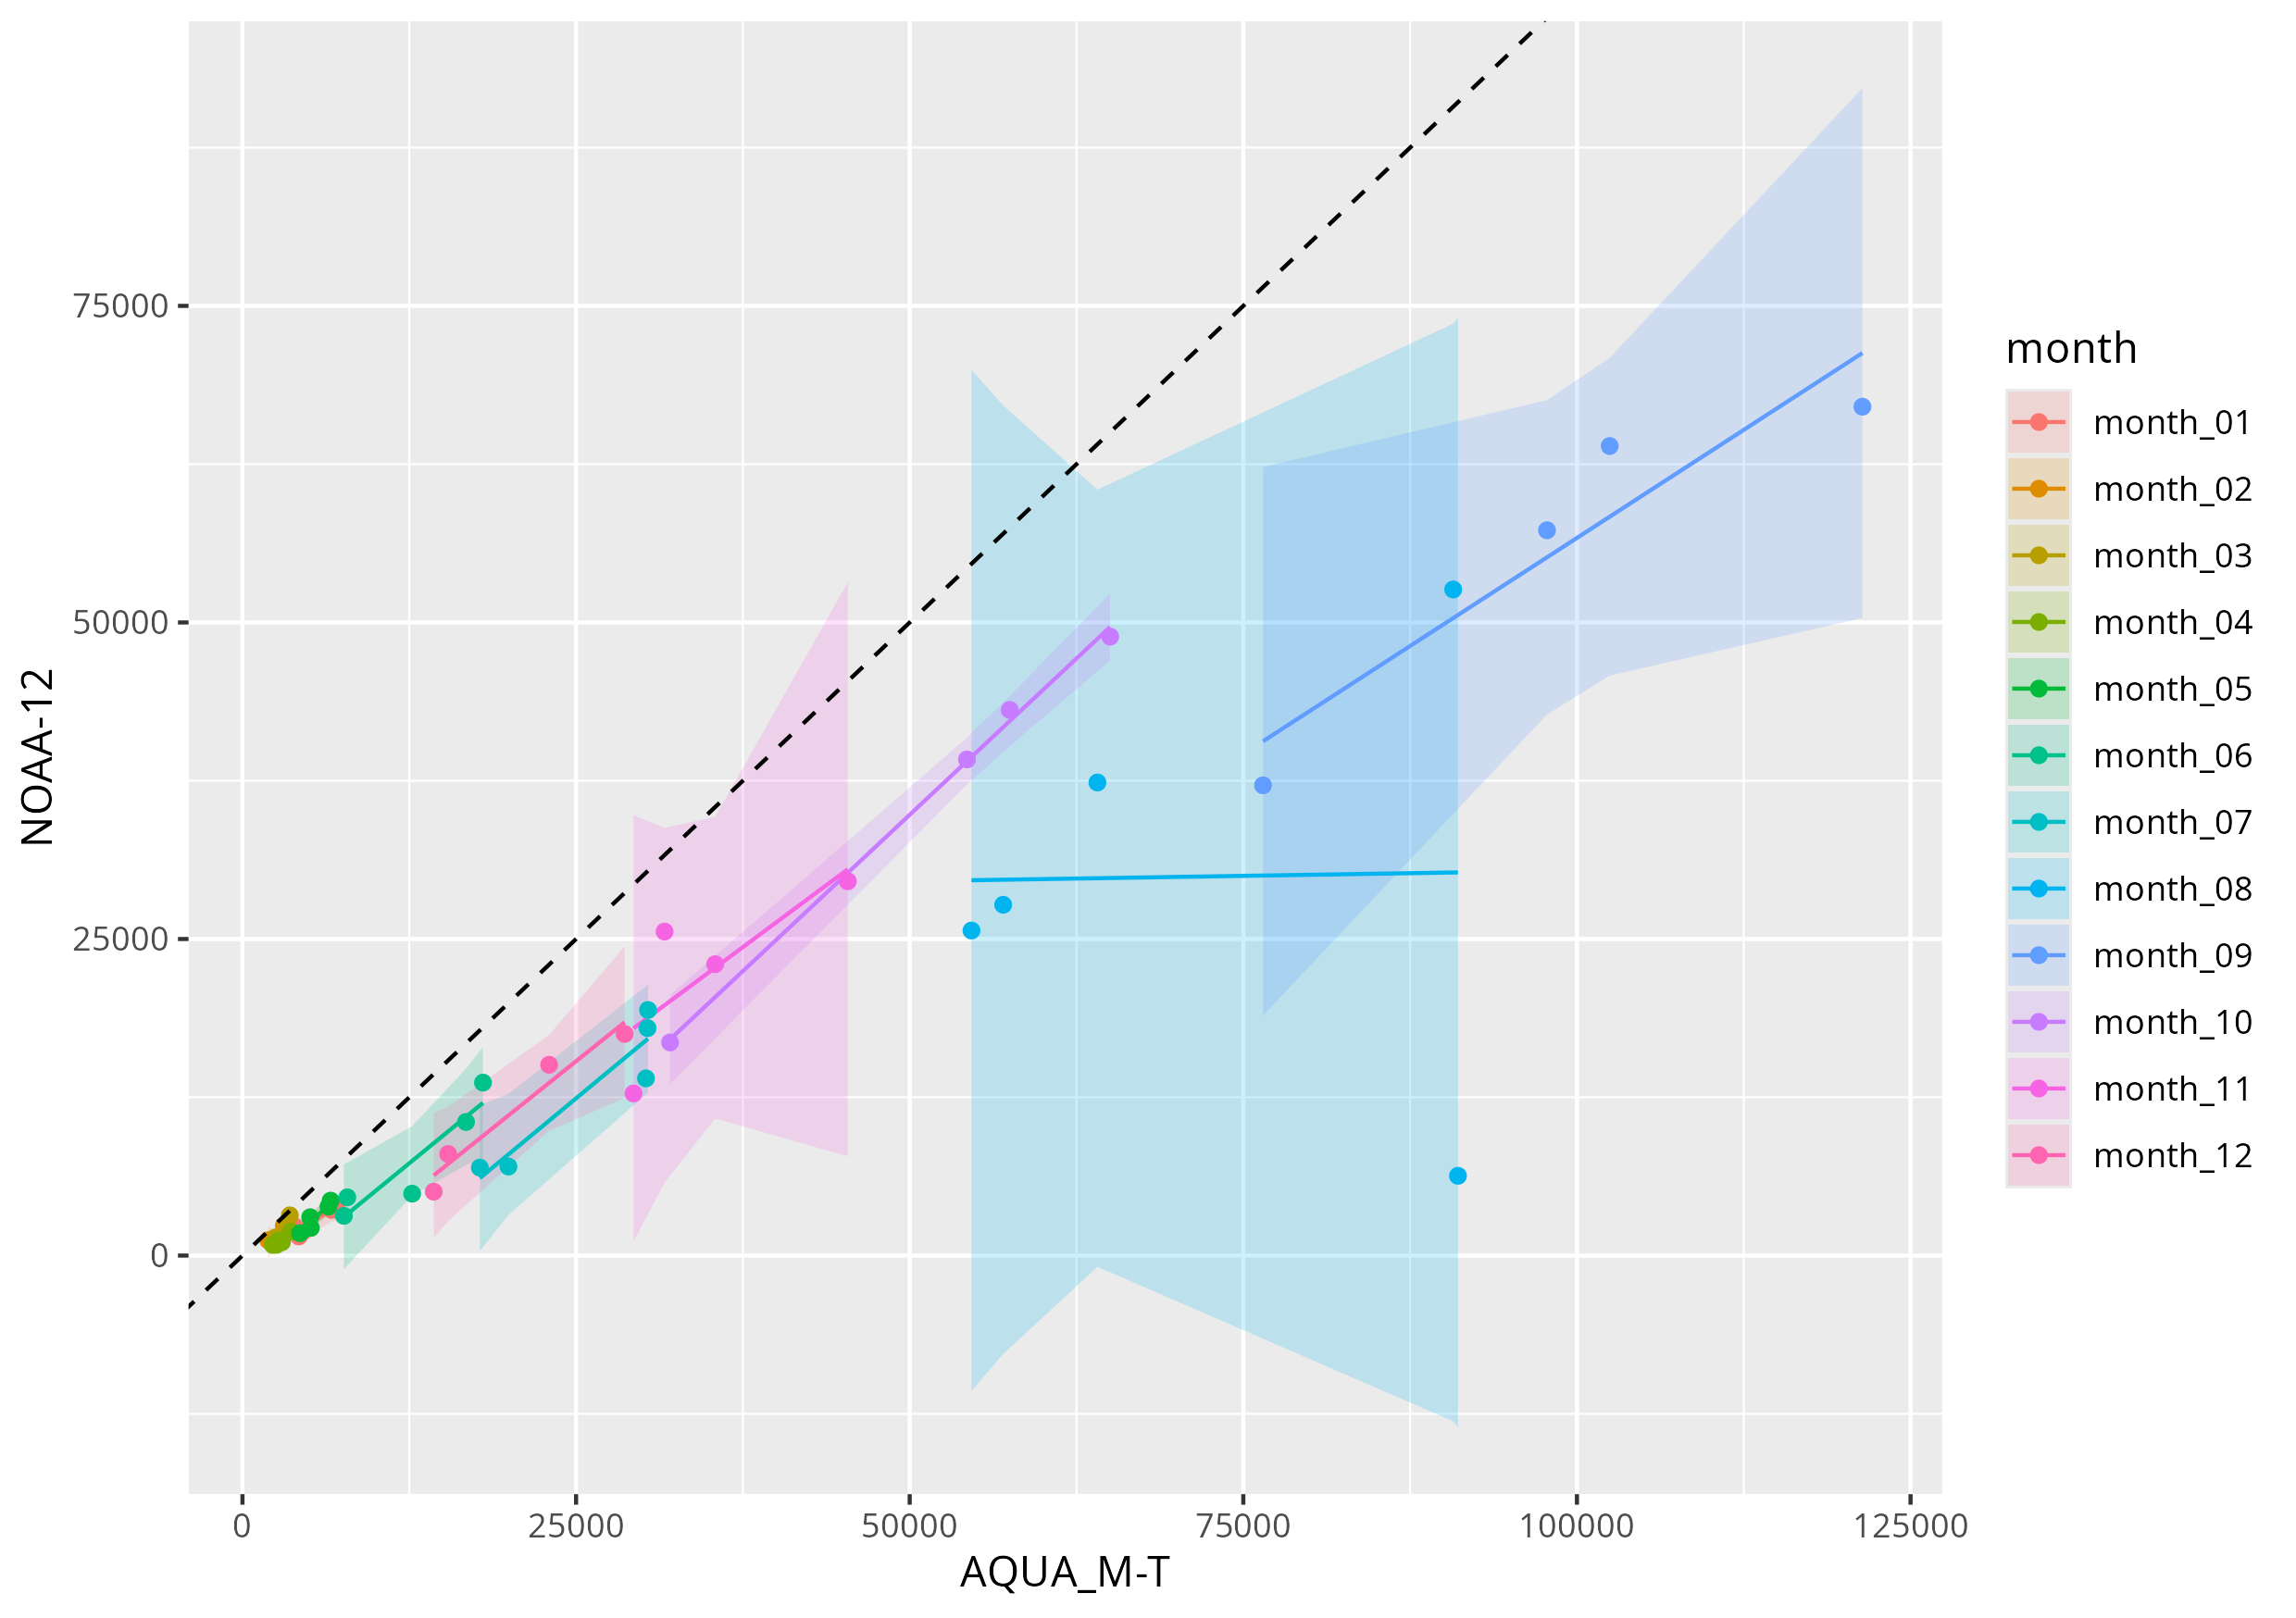
\includegraphics[scale=0.5]
    {figures/plot_queimadas_lm_01_NOAA-12_along_AQUA_M-T.png}
  \end{figure}
\end{frame}

\begin{frame}
  \frametitle{Linear model NPP-375D vs. AQUA\_M-T}
  \begin{figure}
    \centering
    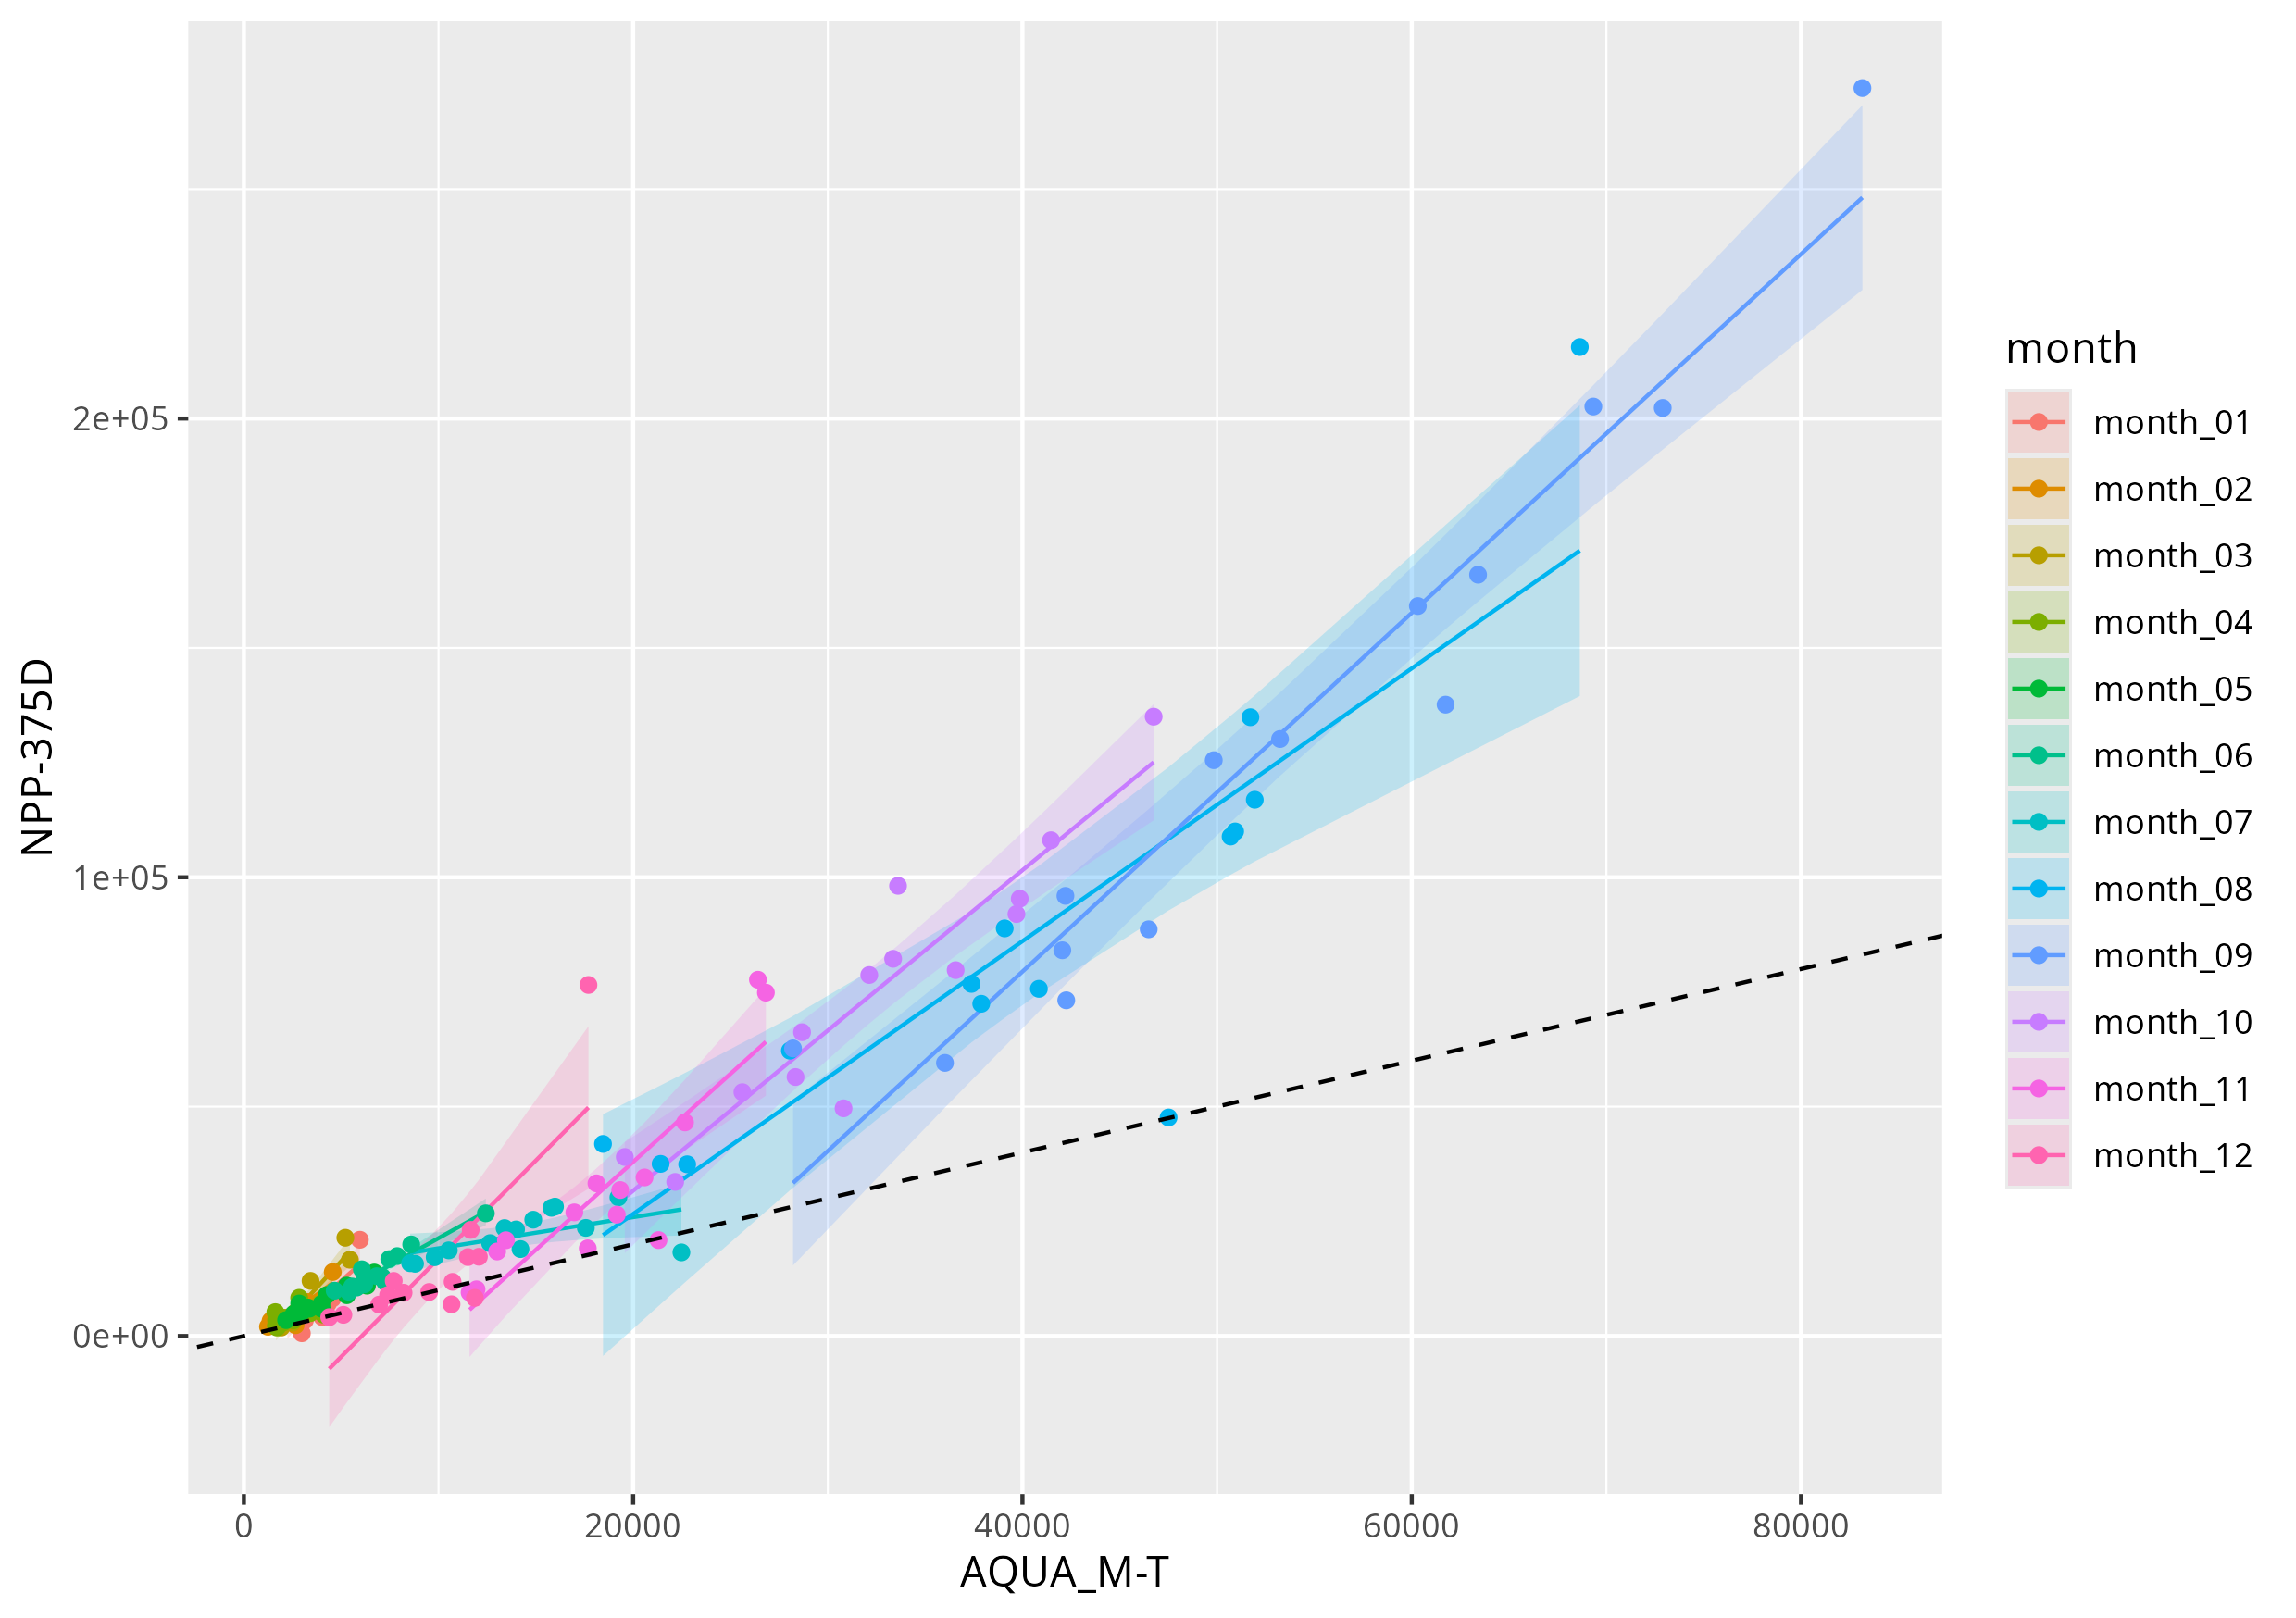
\includegraphics[scale=0.5]
    {figures/plot_queimadas_lm_01_NPP-375D_along_AQUA_M-T.png}
  \end{figure}
\end{frame}

\begin{frame}
  \frametitle{Linear model NPP-375-PM vs. AQUA\_M-T}
  \begin{figure}
    \centering
    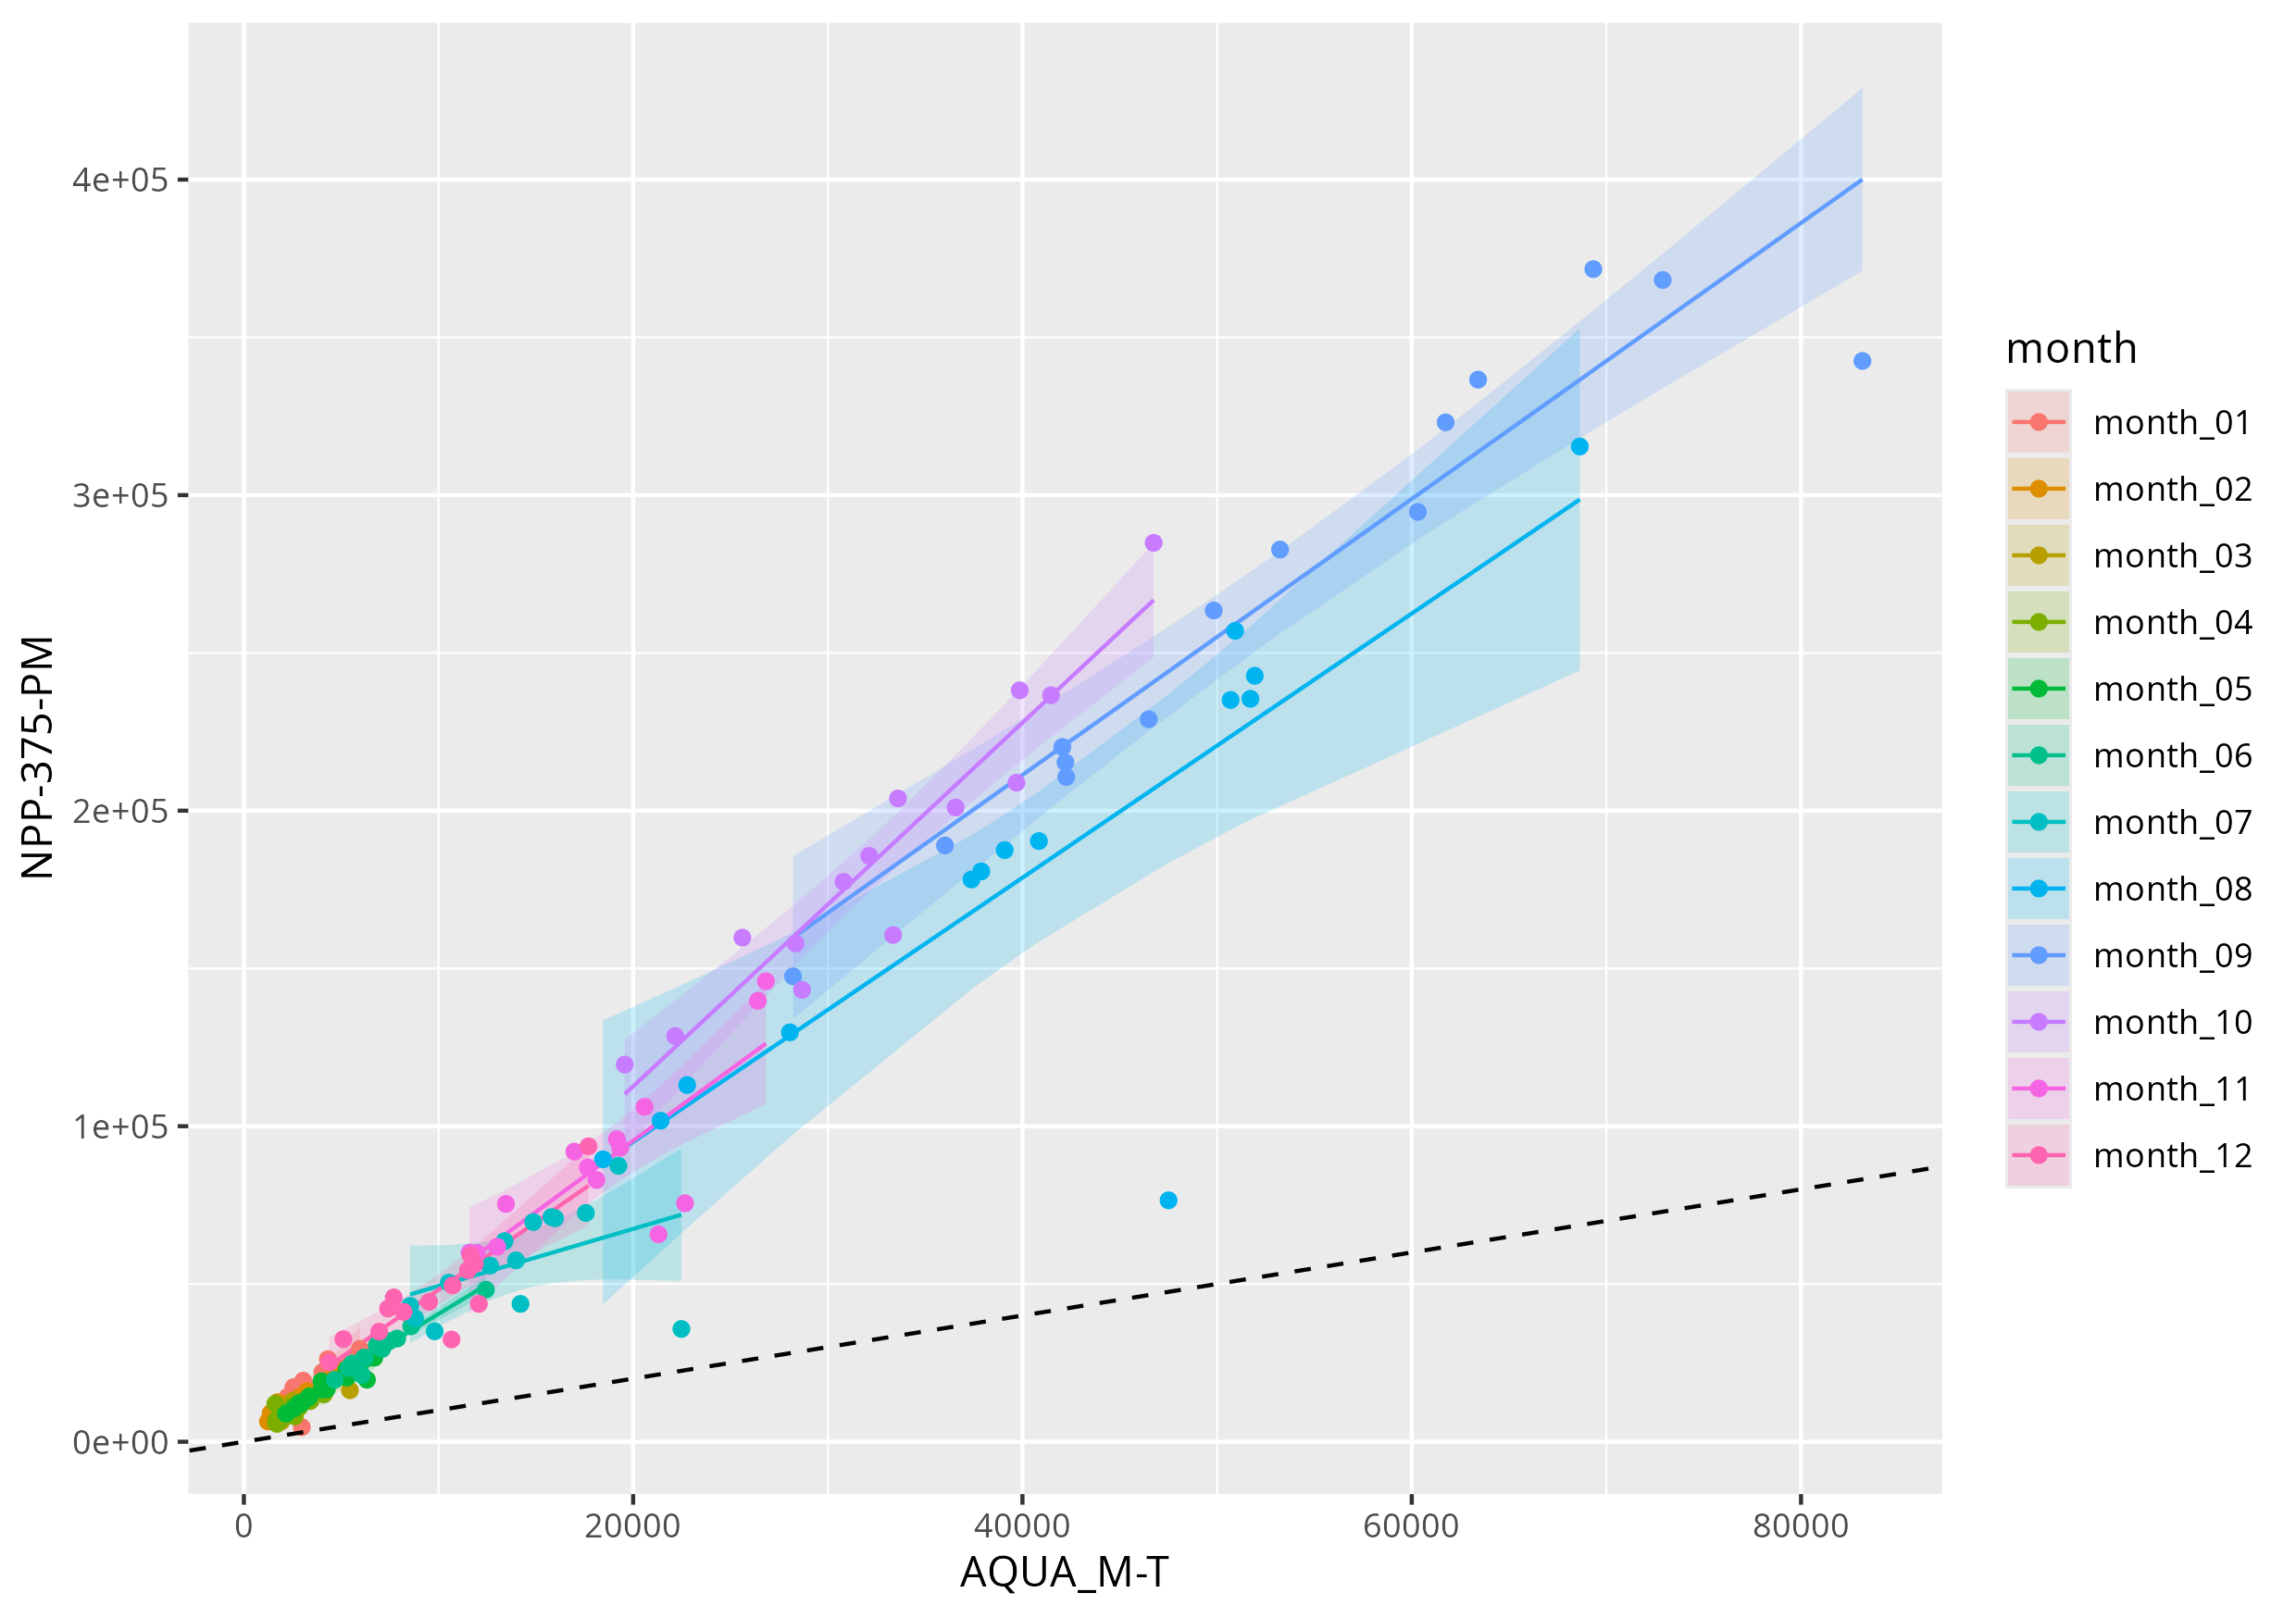
\includegraphics[scale=0.5]
    {figures/plot_queimadas_lm_01_NPP-375-PM_along_AQUA_M-T.png}
  \end{figure}
\end{frame}

\begin{frame}
  \frametitle{Linear model AQUA\_M-T vs. NOAA-12}
  \begin{figure}
    \centering
    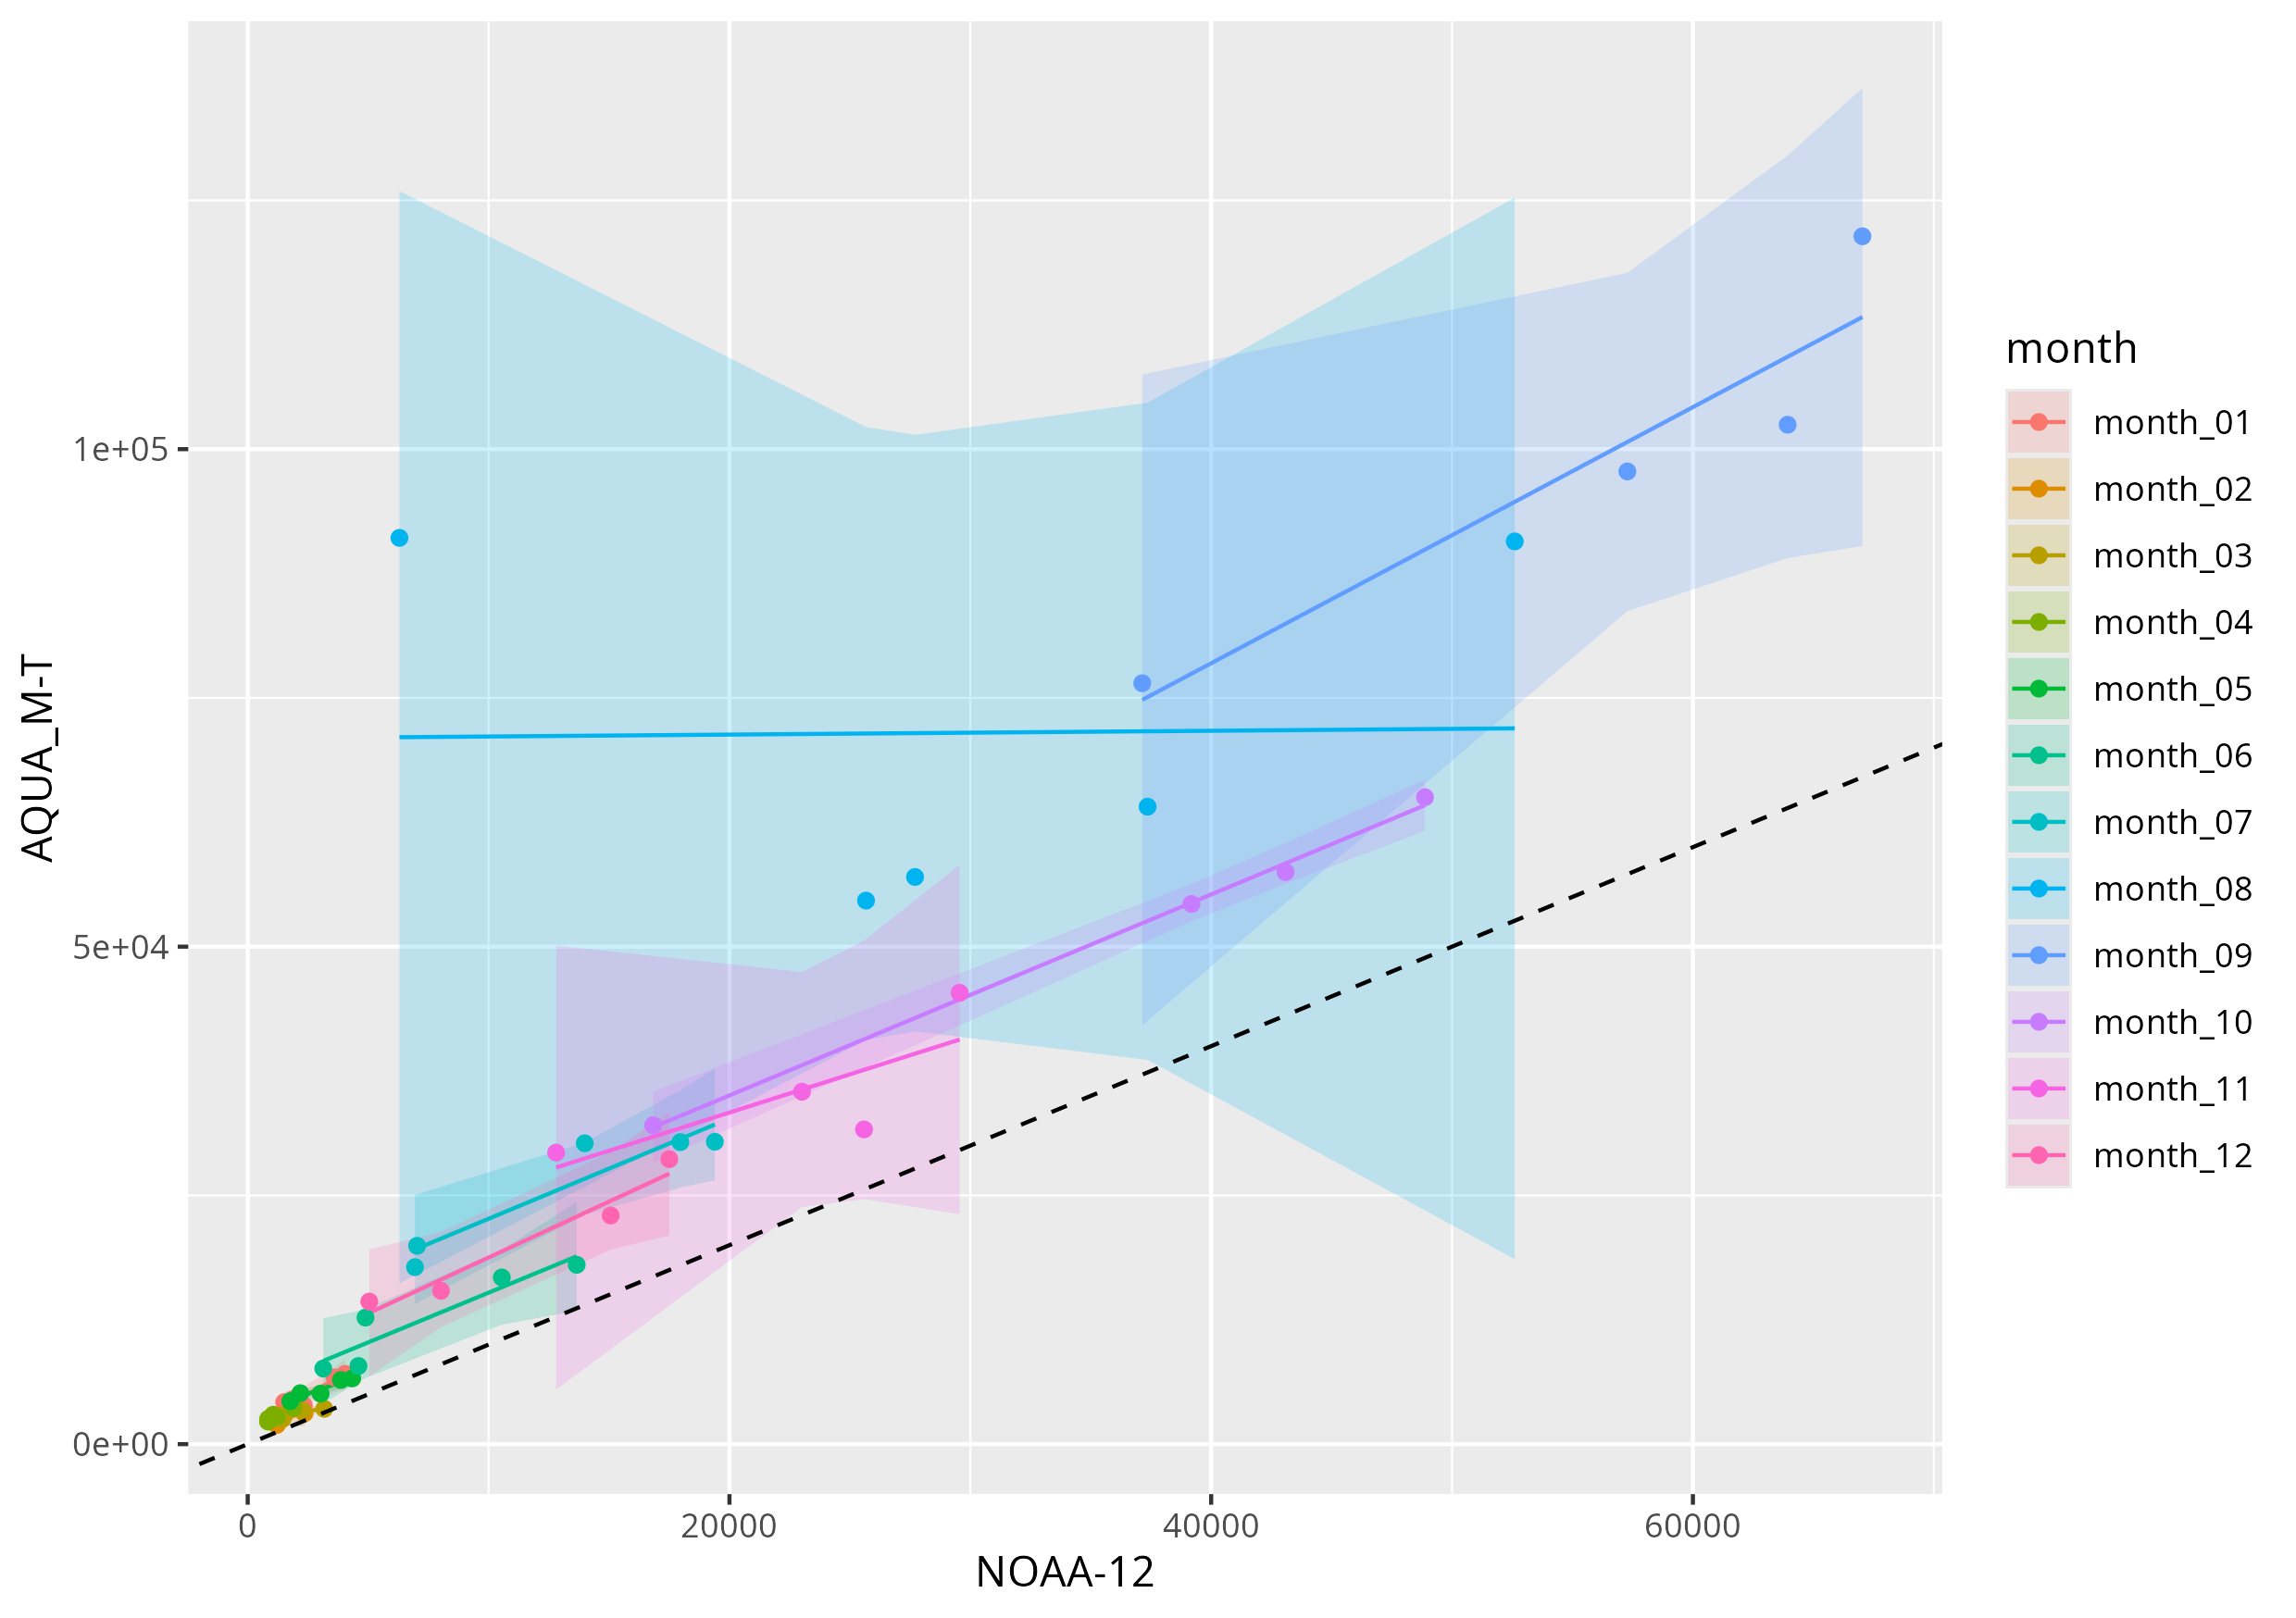
\includegraphics[scale=0.5]
    {figures/plot_queimadas_lm_01_AQUA_M-T_along_NOAA-12.png}
  \end{figure}
\end{frame}

\begin{frame}
  \frametitle{Linear model AQUA\_M-T vs. NPP-375-PM}
  \begin{figure}
    \centering
    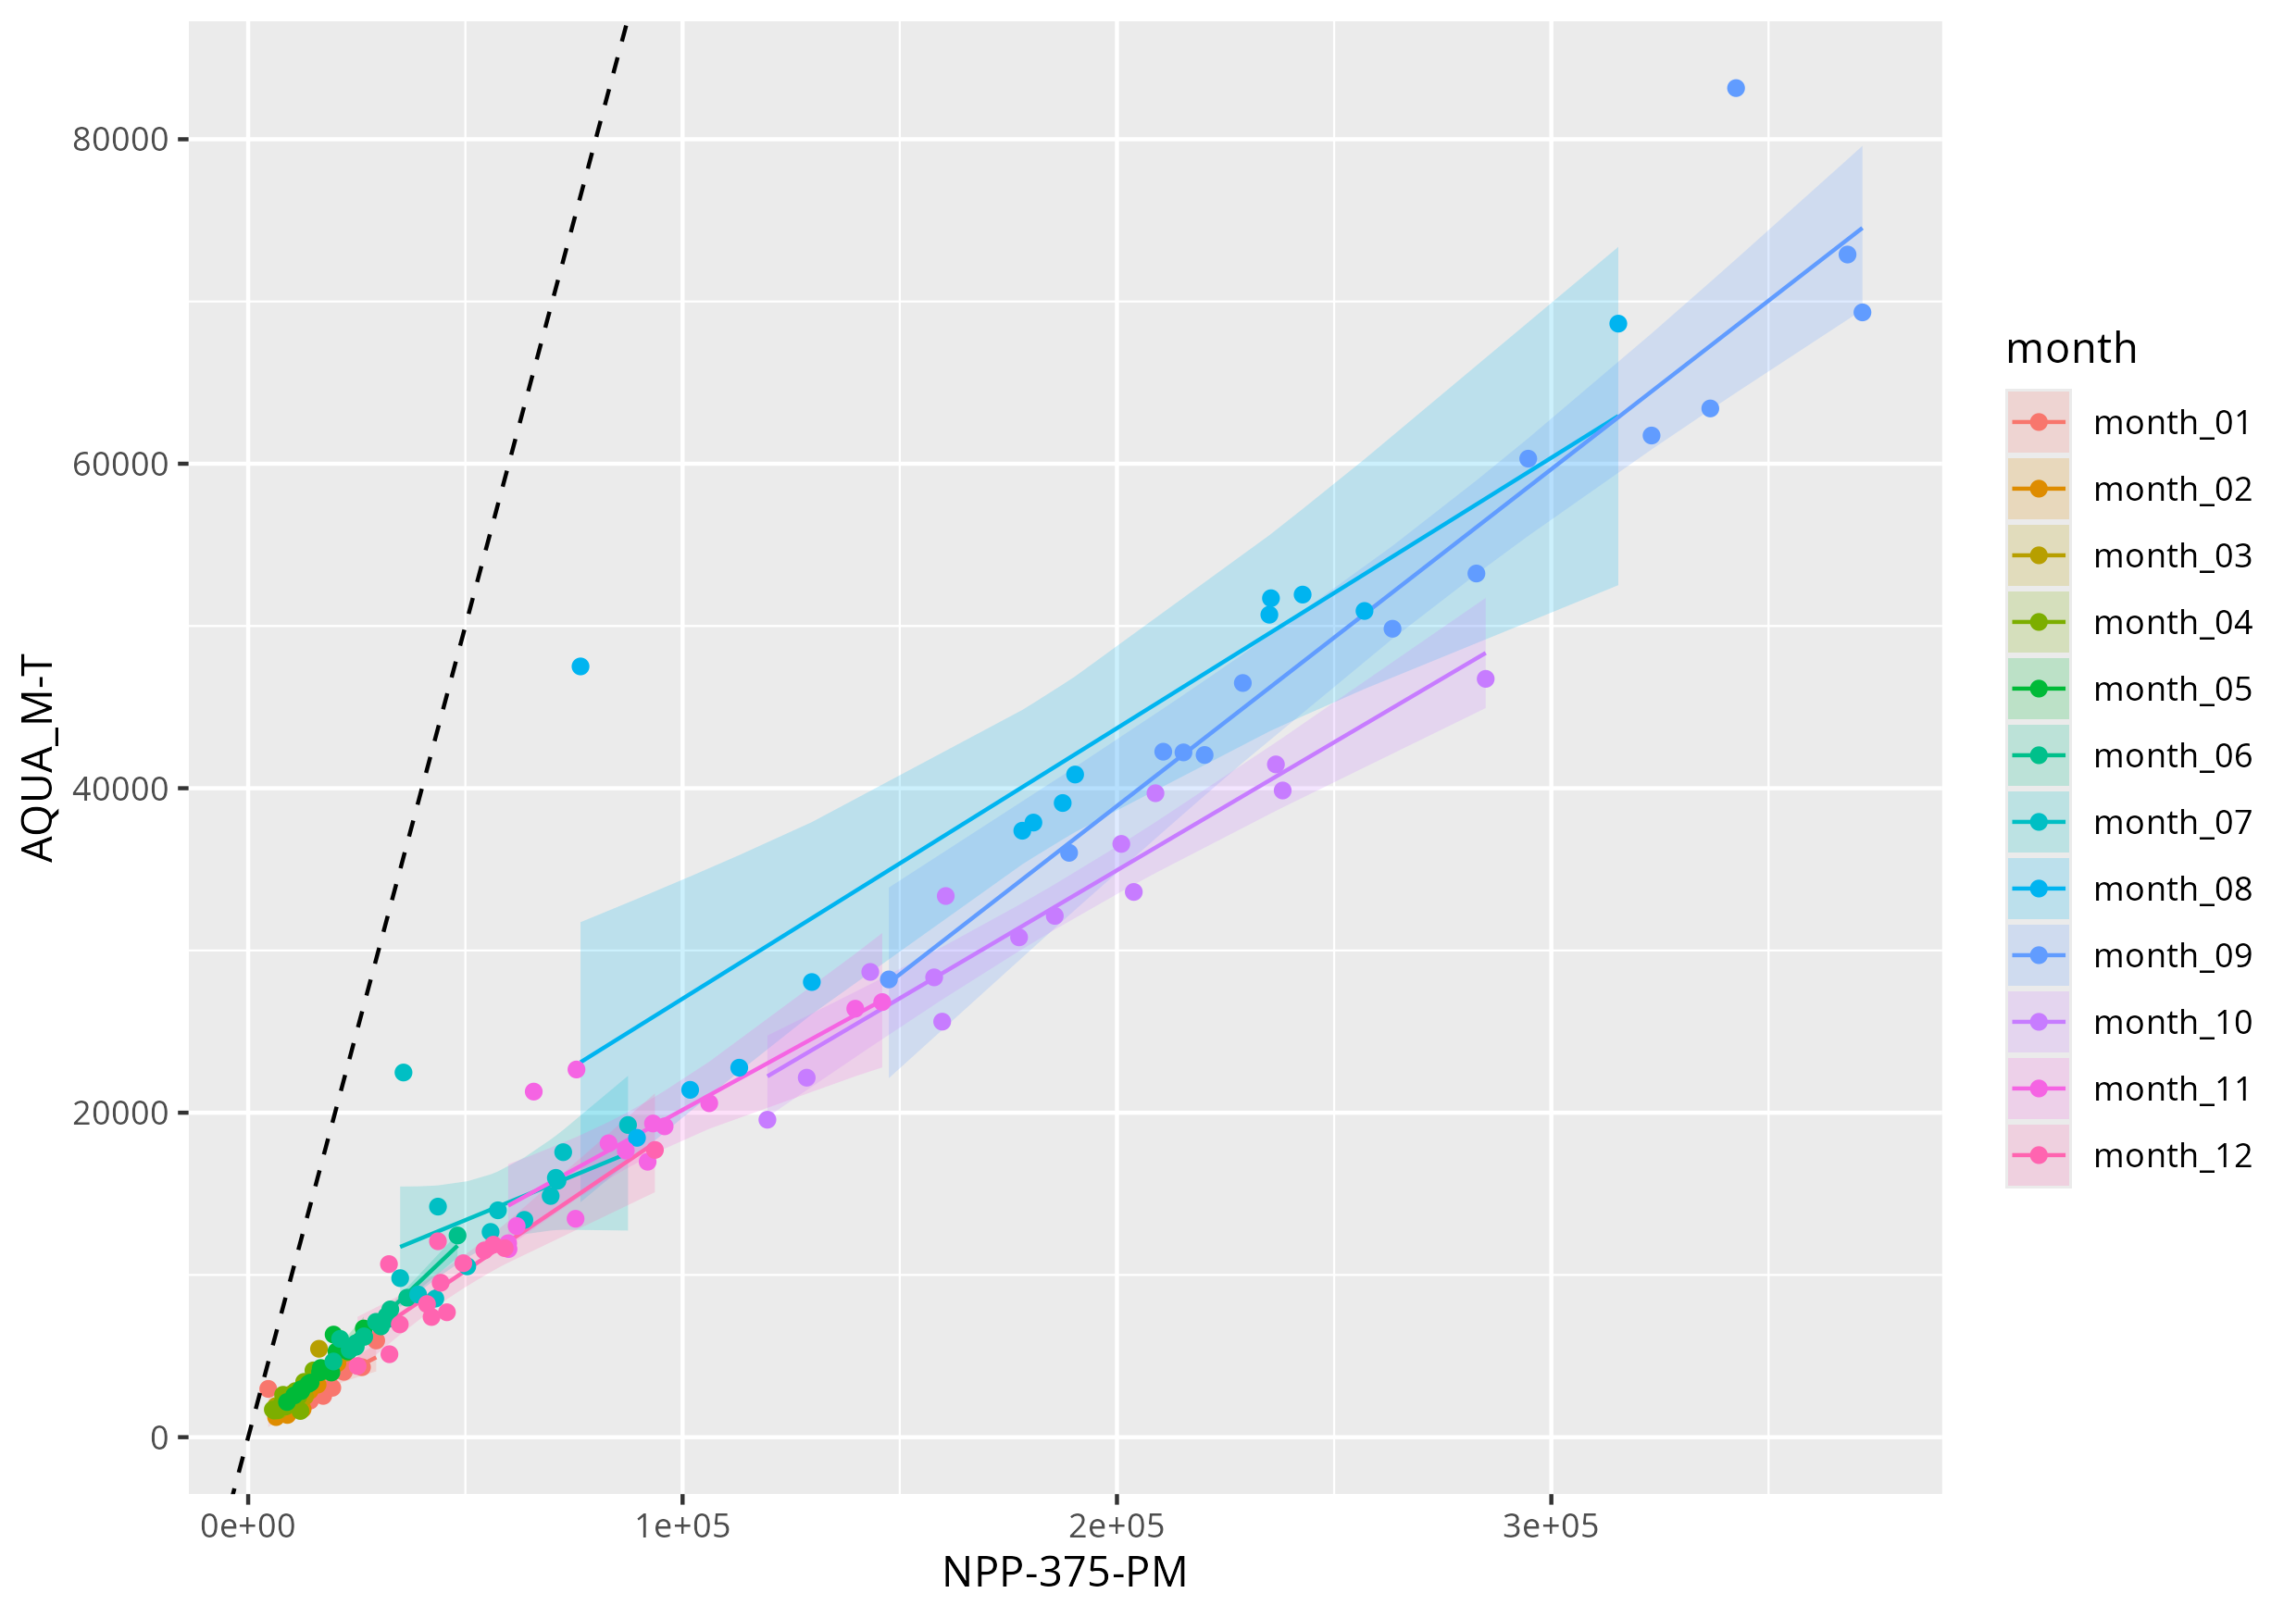
\includegraphics[scale=0.5]
    {figures/plot_queimadas_lm_01_AQUA_M-T_along_NPP-375-PM.png}
  \end{figure}
\end{frame}

\begin{frame}
  \frametitle{Linear model NPP-375D vs. NPP-375-PM}
  \begin{figure}
    \centering
    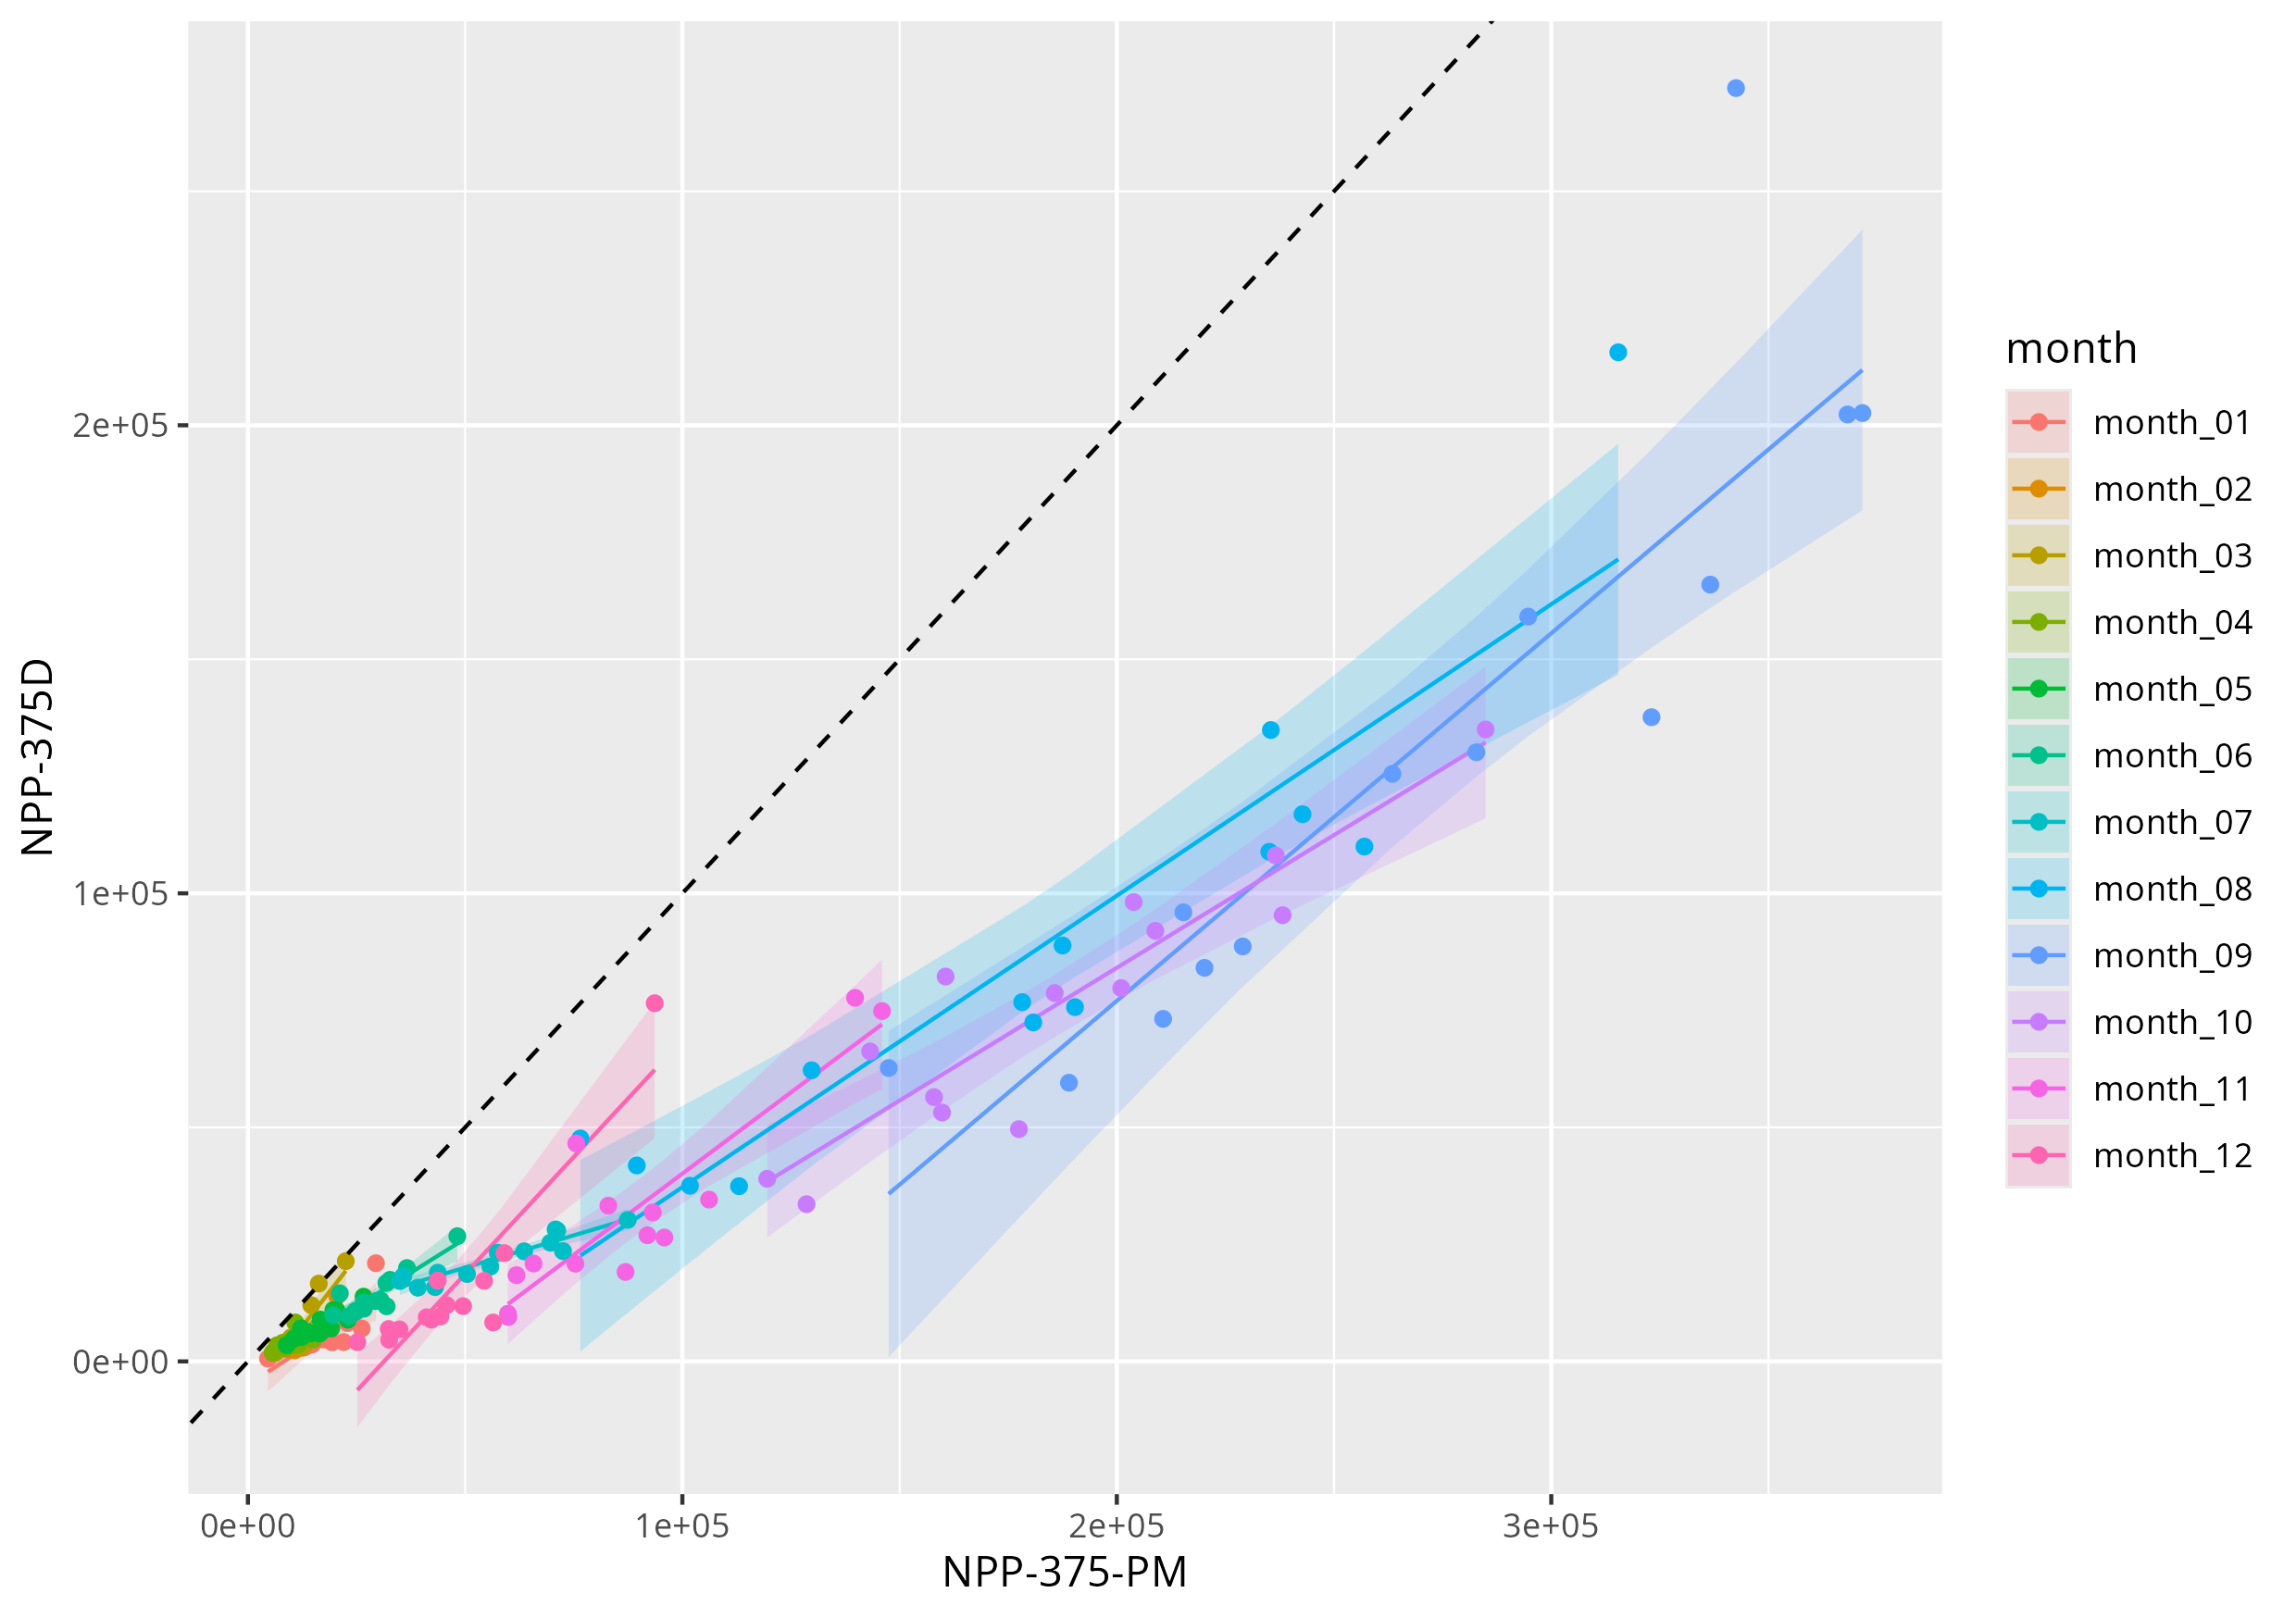
\includegraphics[scale=0.5]
    {figures/plot_queimadas_lm_01_NPP-375D_along_NPP-375-PM.png}
  \end{figure}
\end{frame}

\begin{frame}
  \frametitle{Linear model AQUA\_M-T vs. NPP-375D}
  \begin{figure}
    \centering
    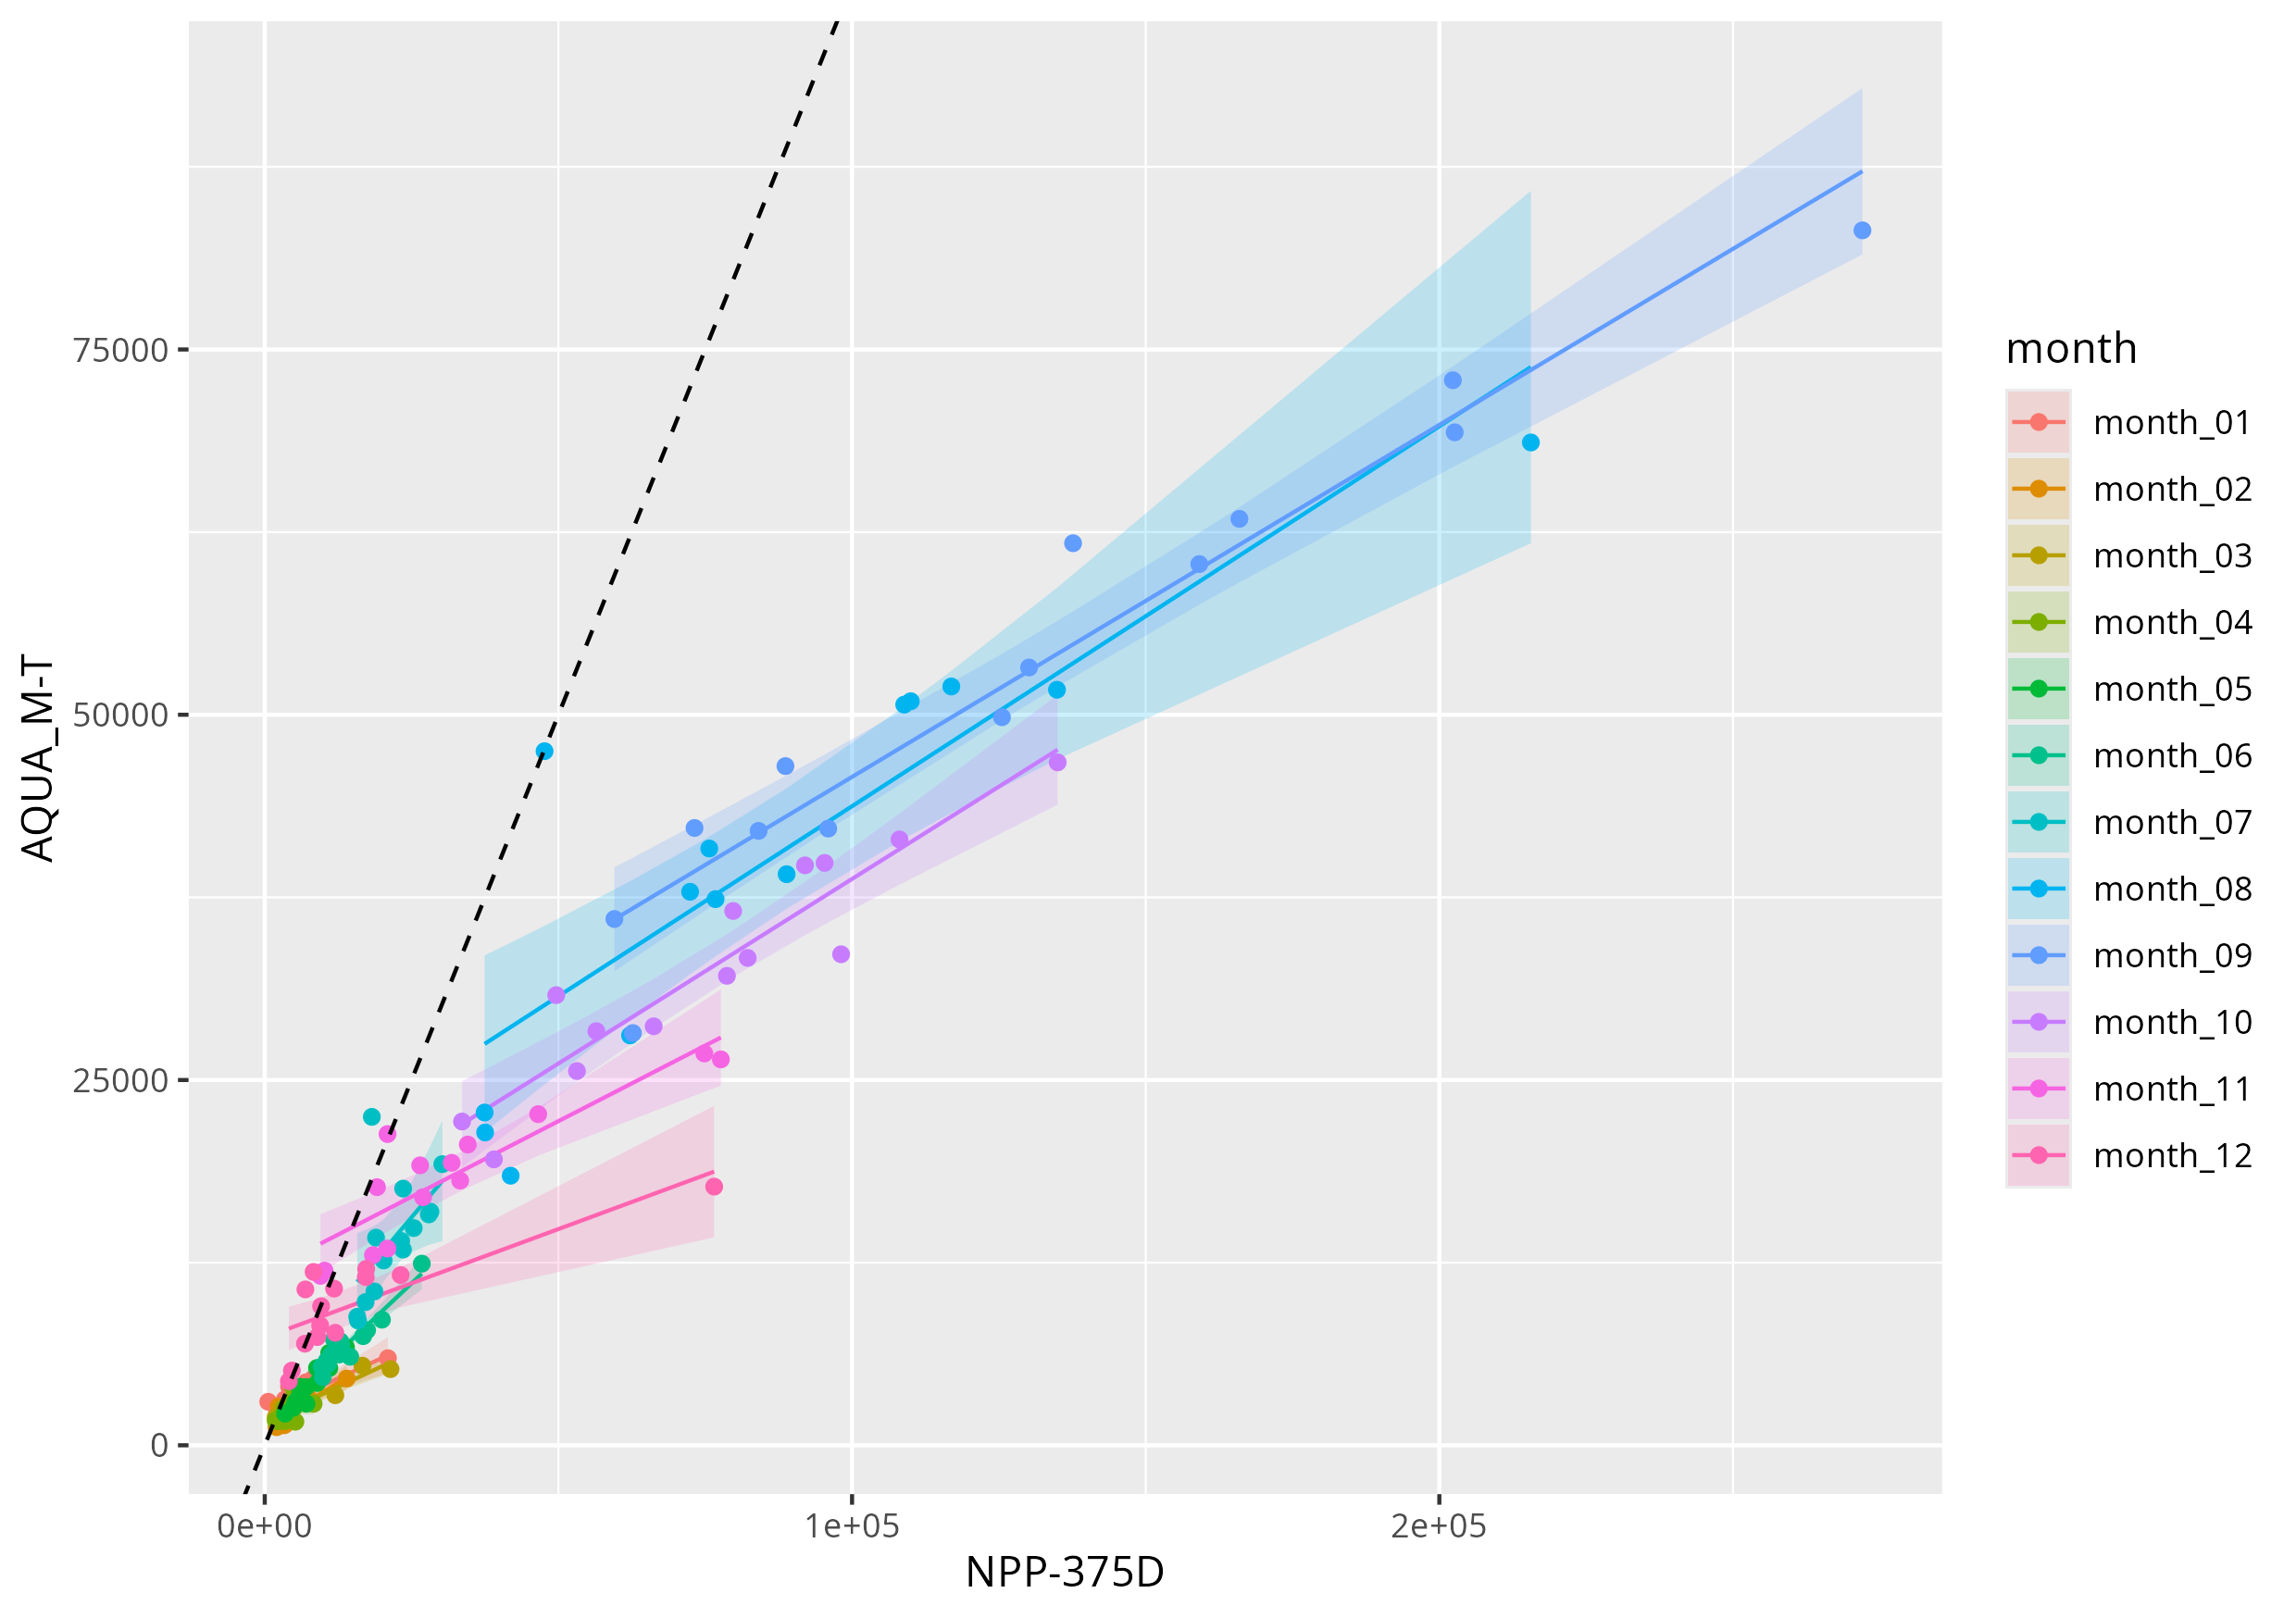
\includegraphics[scale=0.5]
    {figures/plot_queimadas_lm_01_AQUA_M-T_along_NPP-375D.png}
  \end{figure}
\end{frame}

\begin{frame}
  \frametitle{Linear model NPP-375-PM vs. NPP-375D}
  \begin{figure}
    \centering
    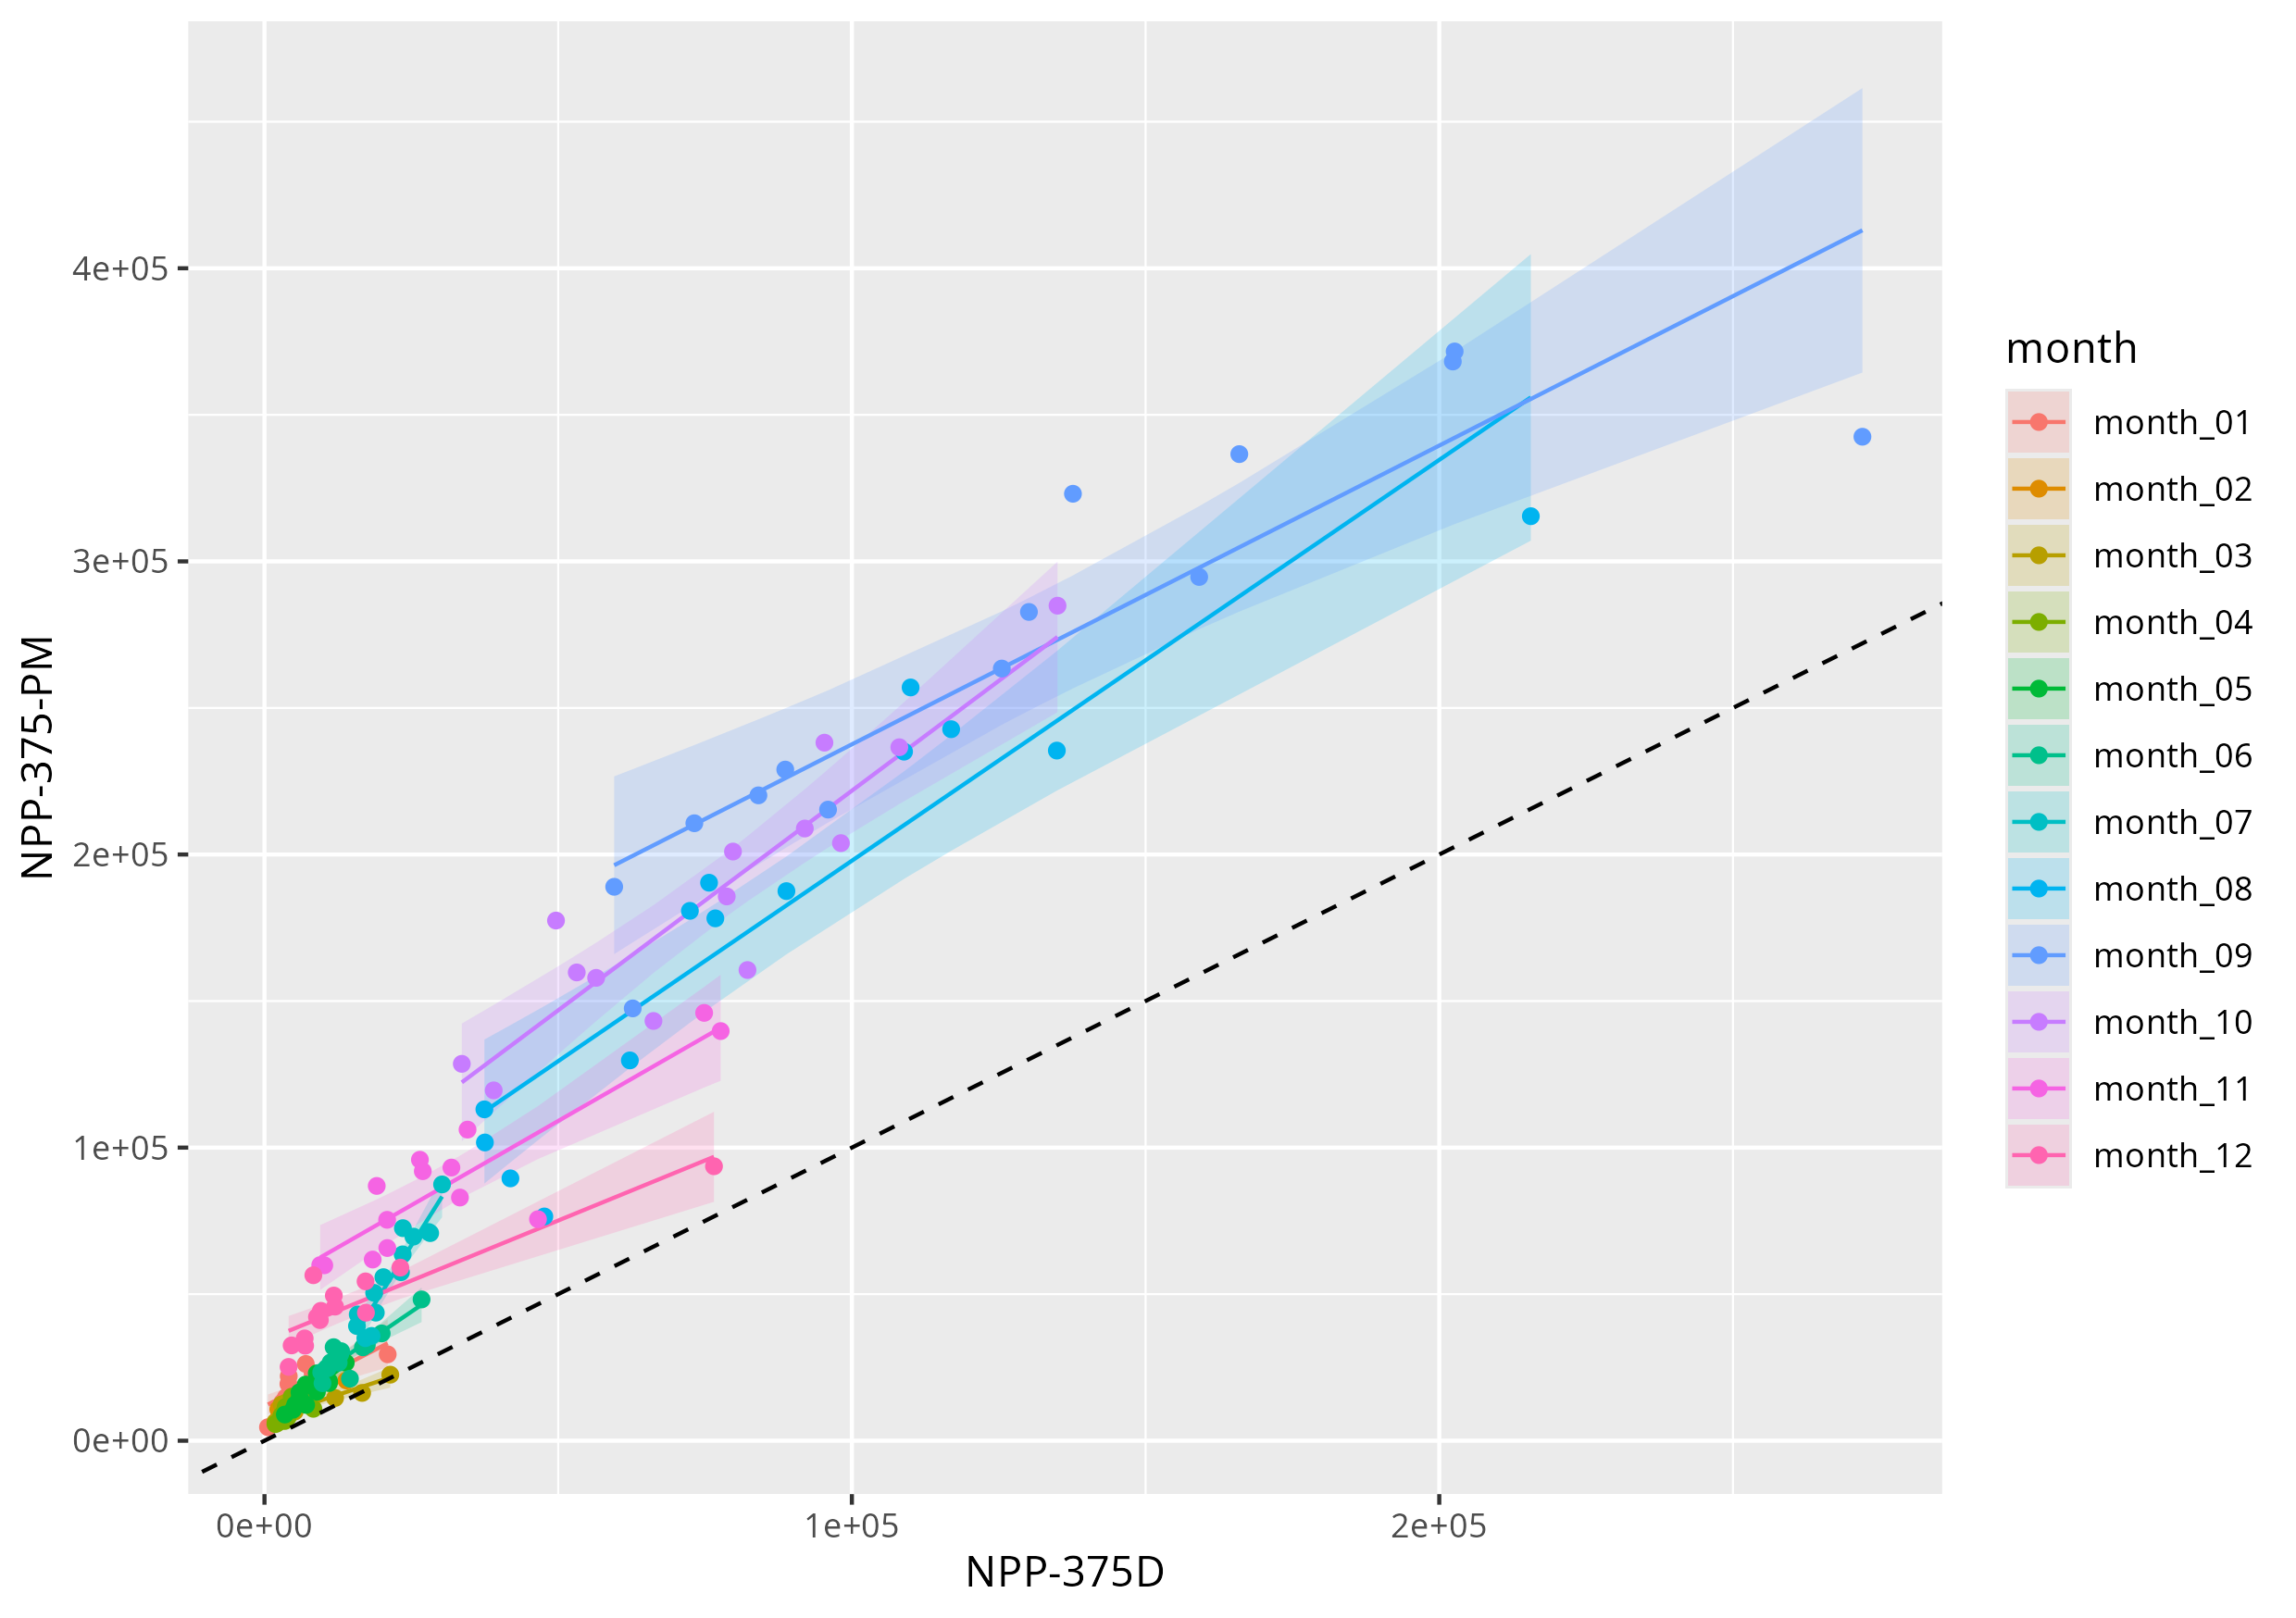
\includegraphics[scale=0.5]
    {figures/plot_queimadas_lm_01_NPP-375-PM_along_NPP-375D.png}
  \end{figure}
\end{frame}

\subsection{Forecast}

\begin{frame}
  \frametitle{Stretch NOAA-12 to match AQUA\_M-T (month-by-month)}
  \begin{figure}
    \centering
    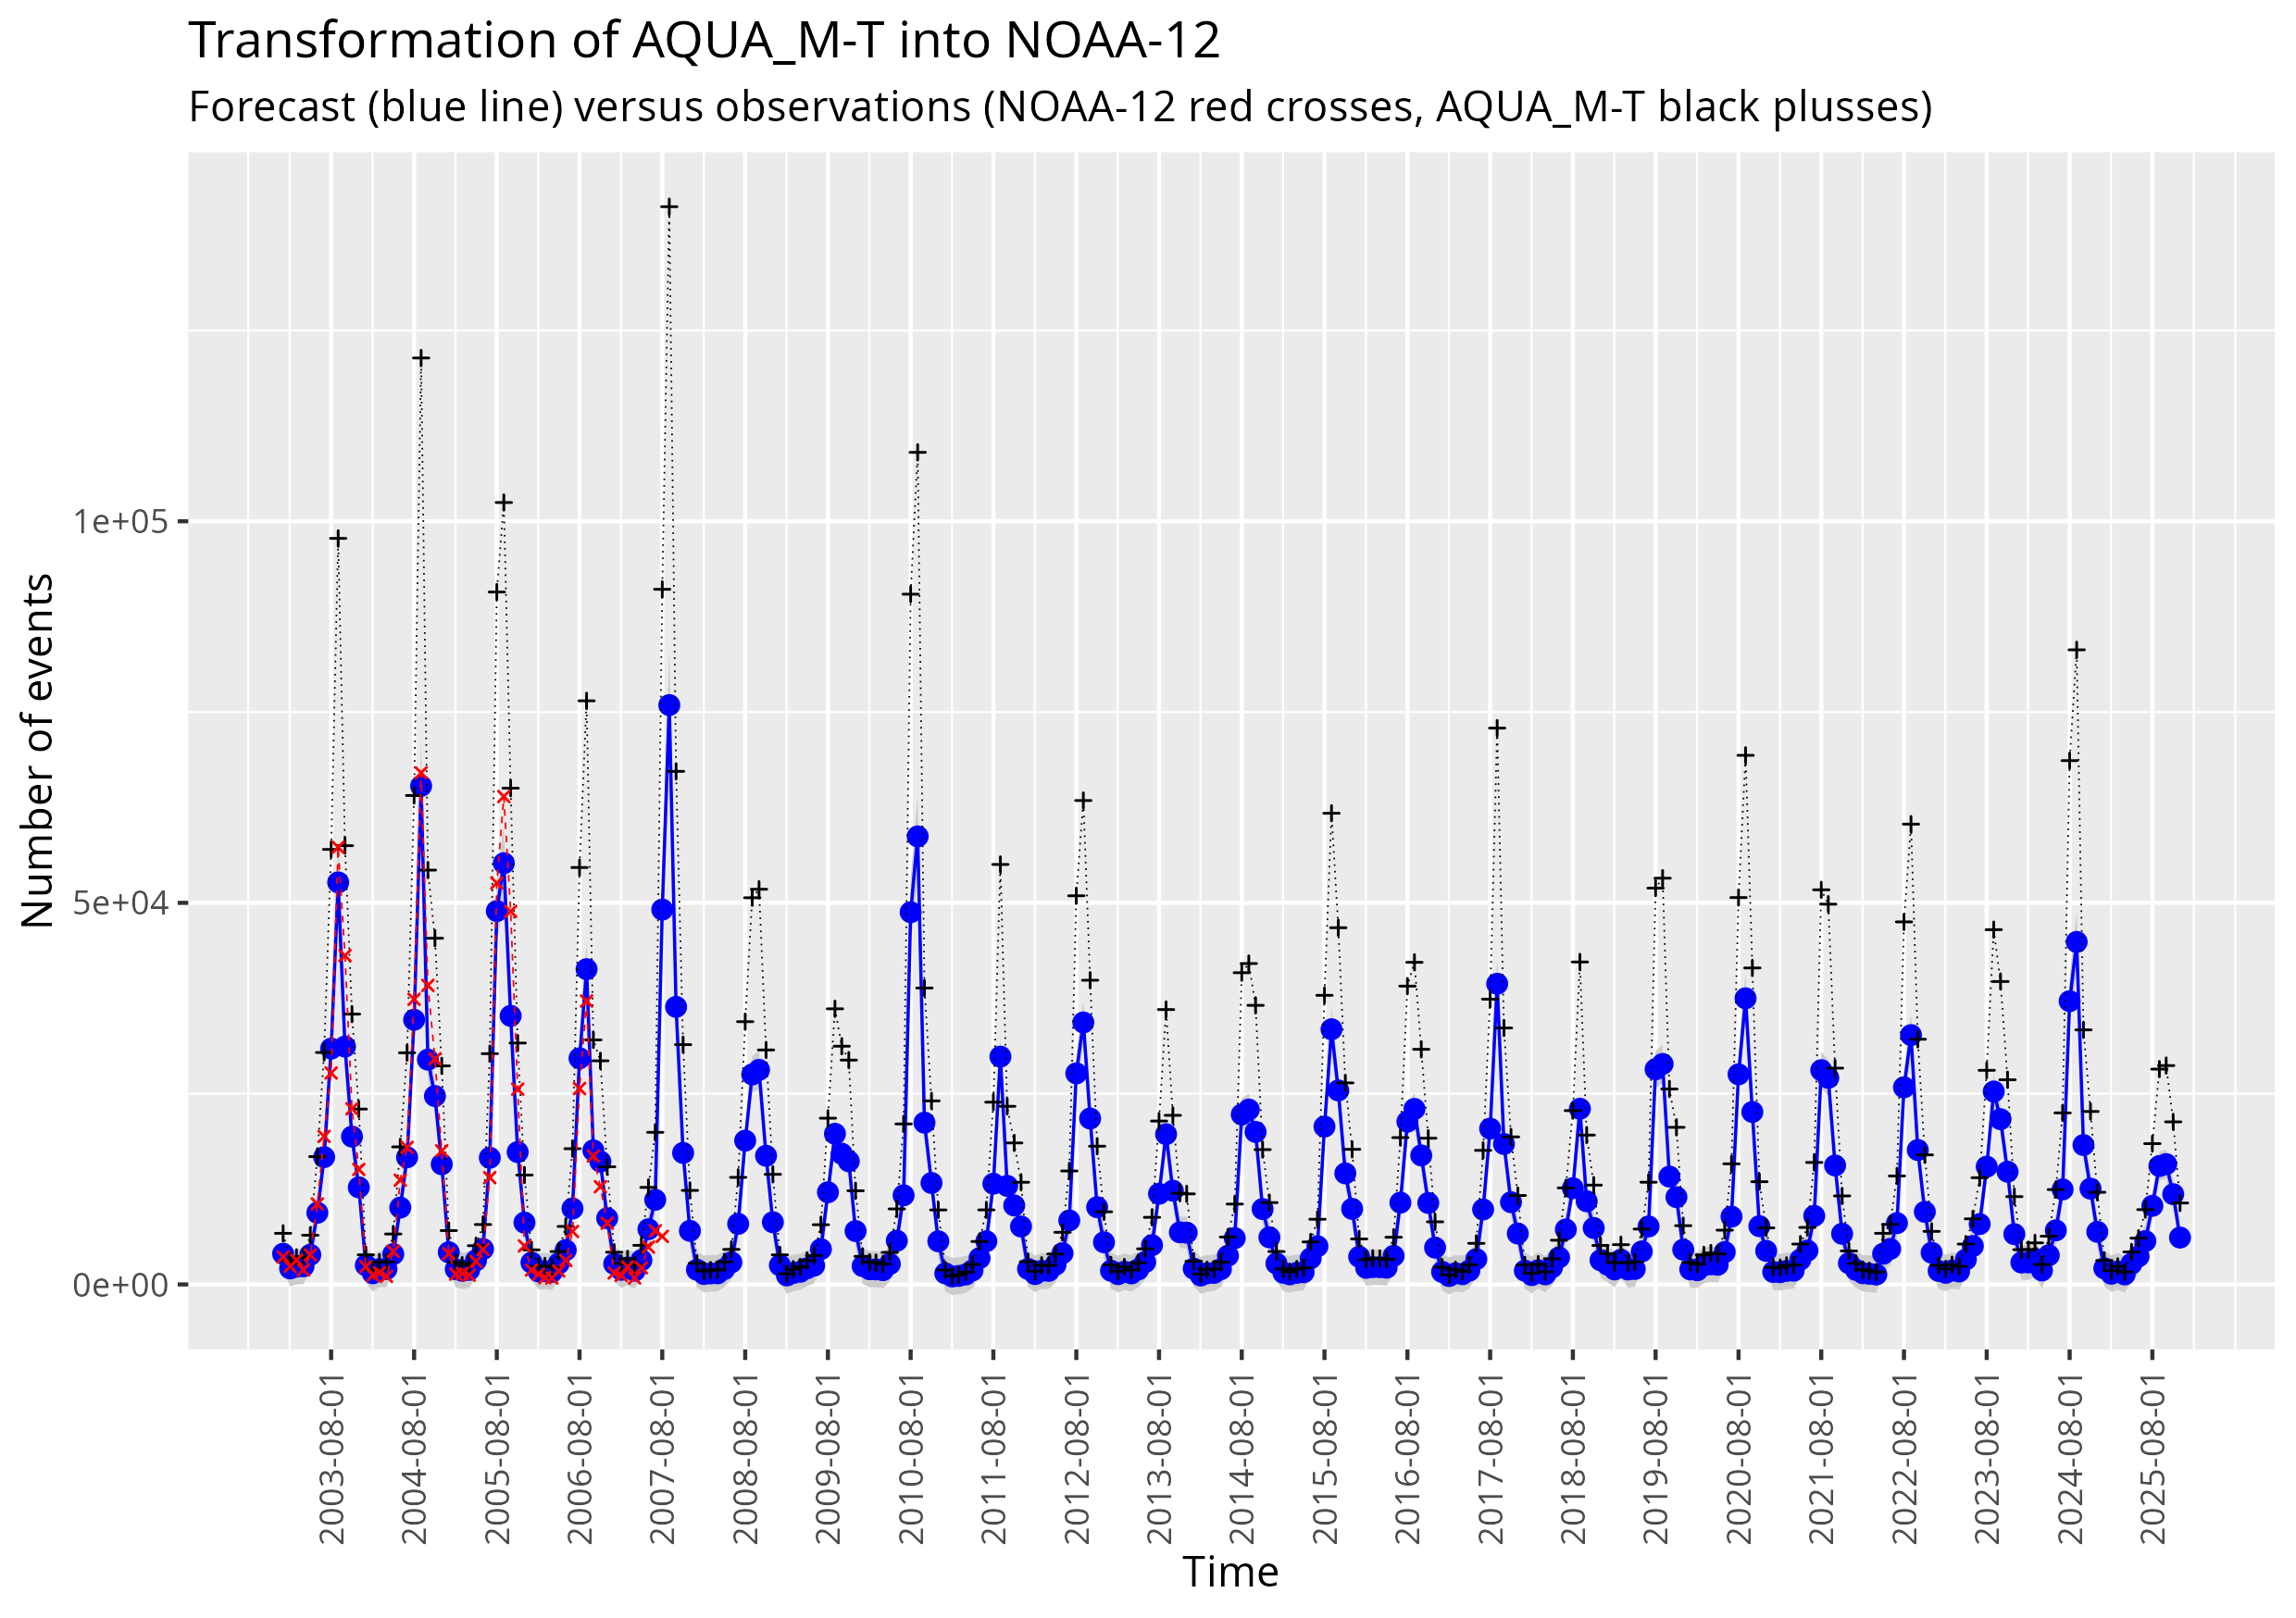
\includegraphics[scale=0.5]
    {figures/plot_forecast_01_NOAA-12_along_AQUA_M-T.png}
  \end{figure}
\end{frame}

\begin{frame}
  \frametitle{Stretch NPP-375D to match AQUA\_M-T (month-by-month)}
  \begin{figure}
    \centering
    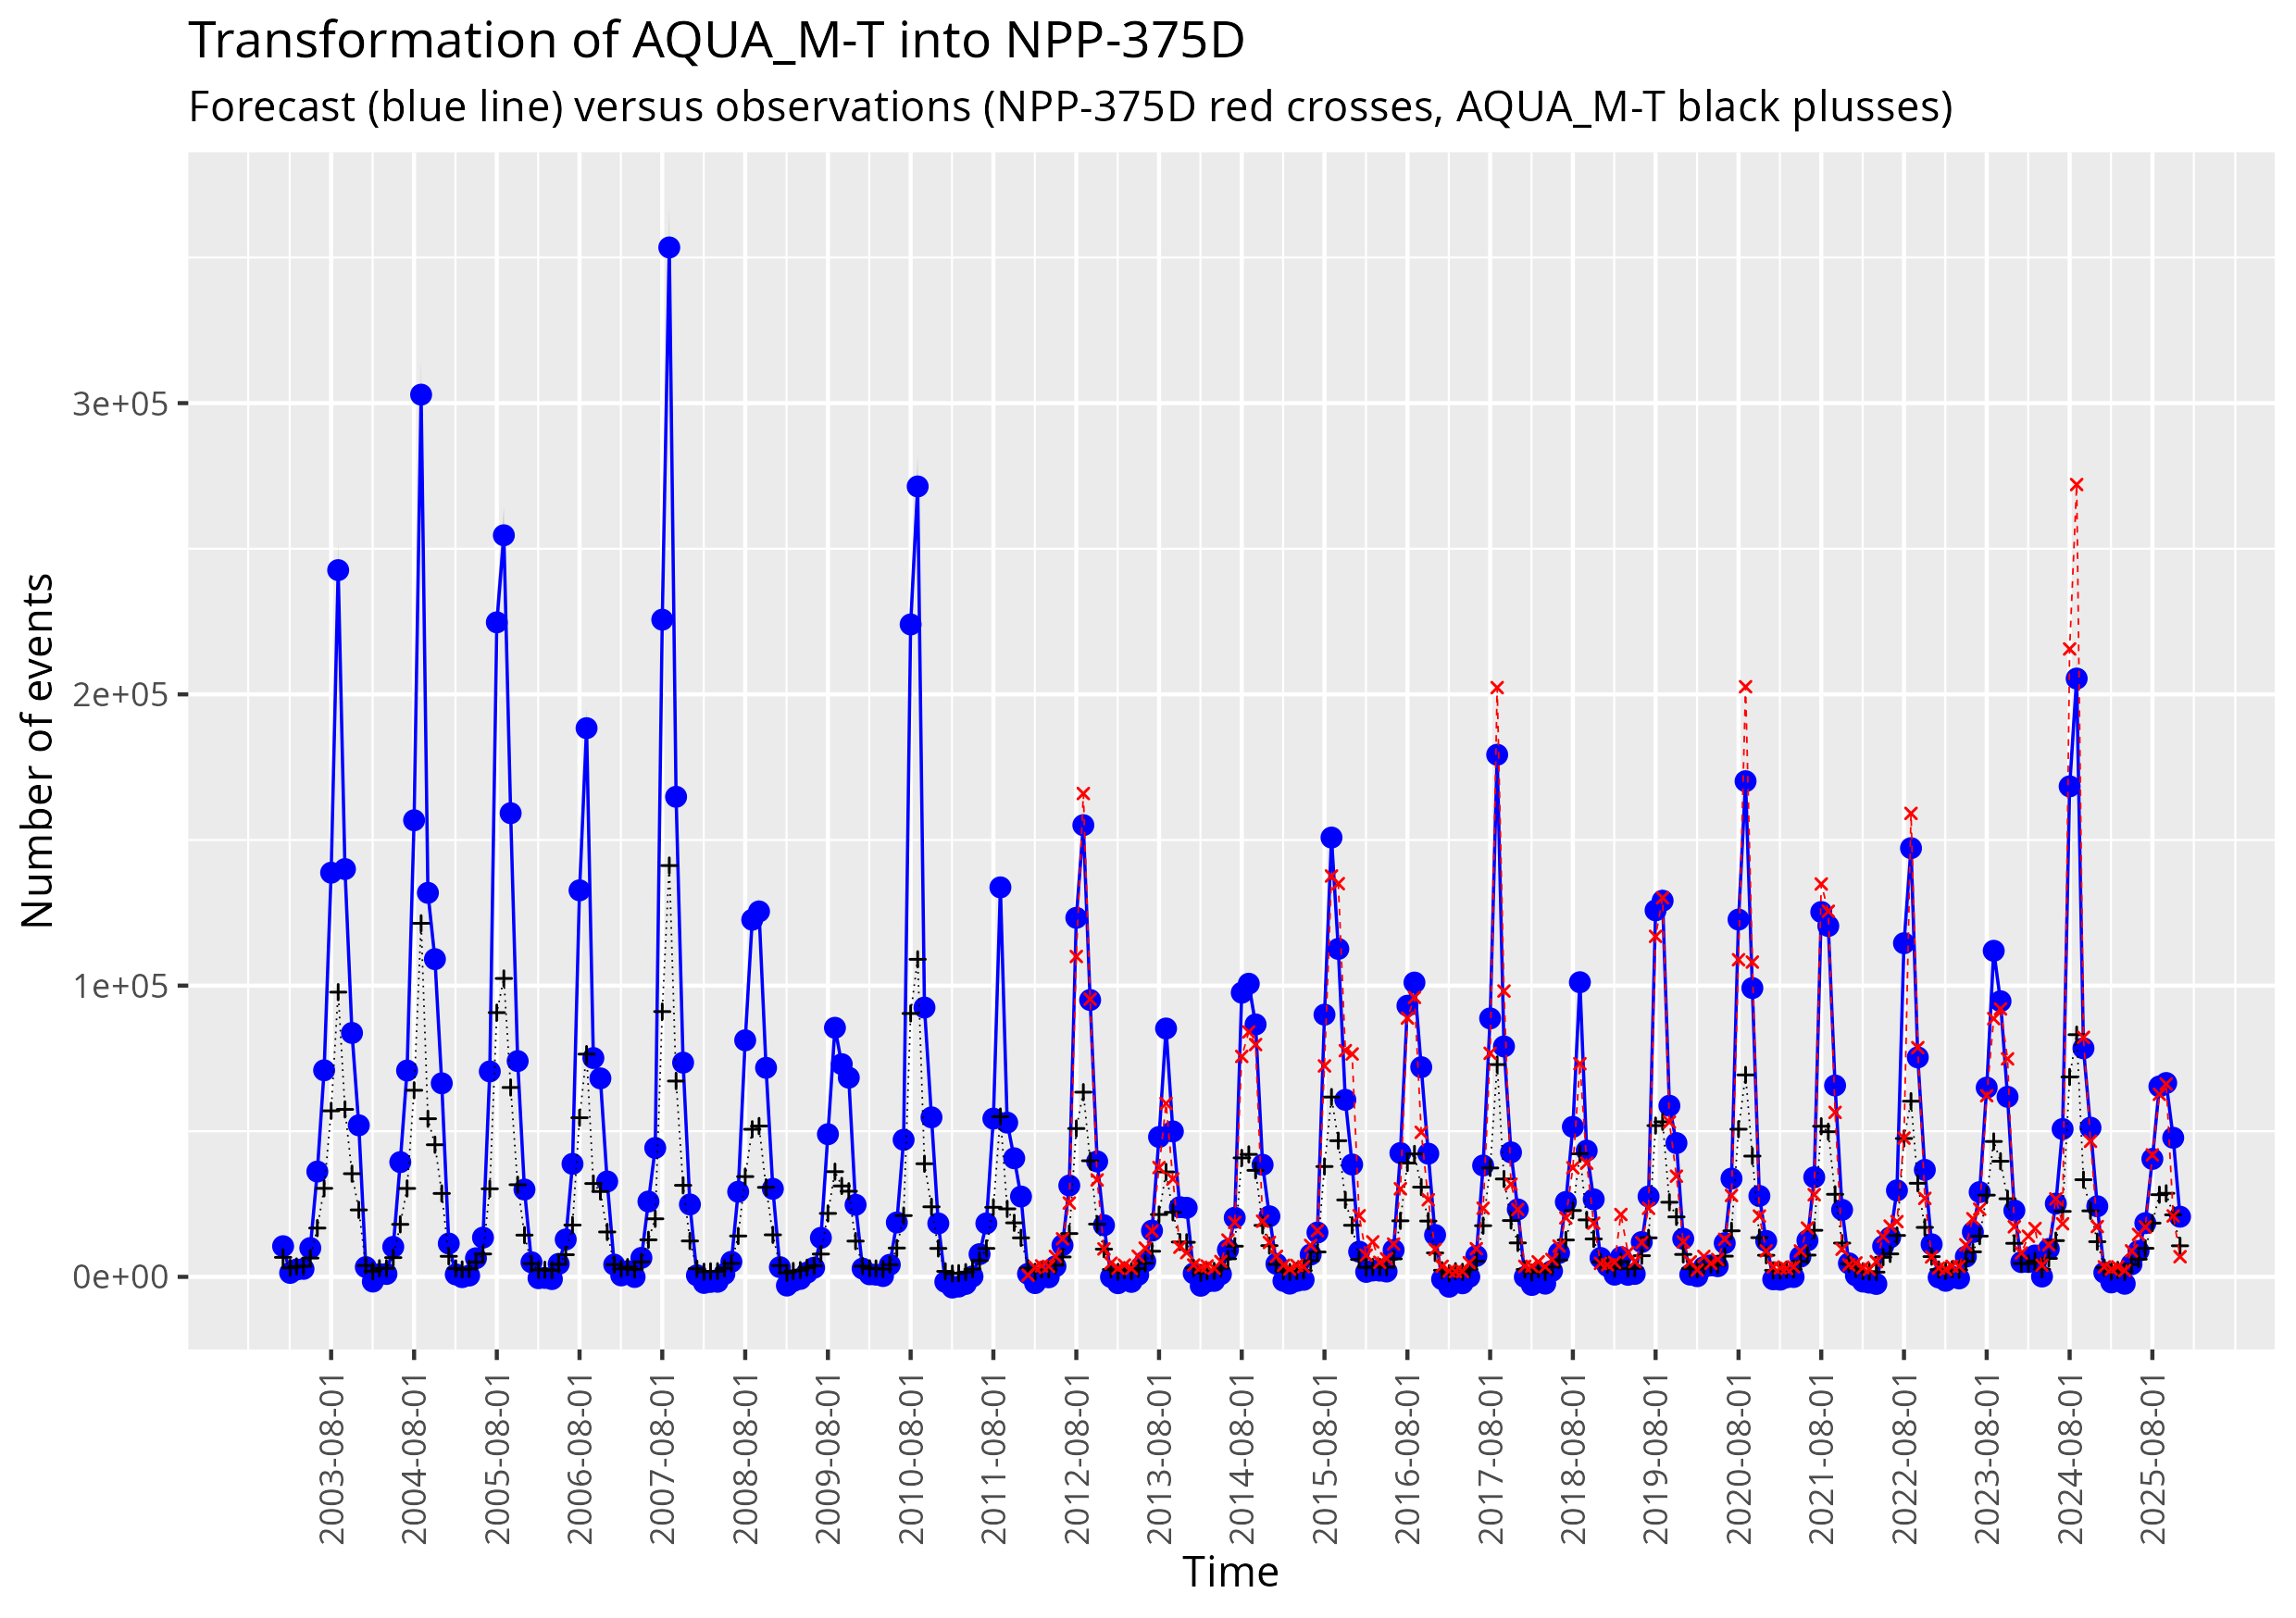
\includegraphics[scale=0.5]
    {figures/plot_forecast_01_NPP-375D_along_AQUA_M-T.png}
  \end{figure}
\end{frame}

\begin{frame}
  \frametitle{Stretch NPP-375-PM to match AQUA\_M-T (month-by-month)}
  \begin{figure}
    \centering
    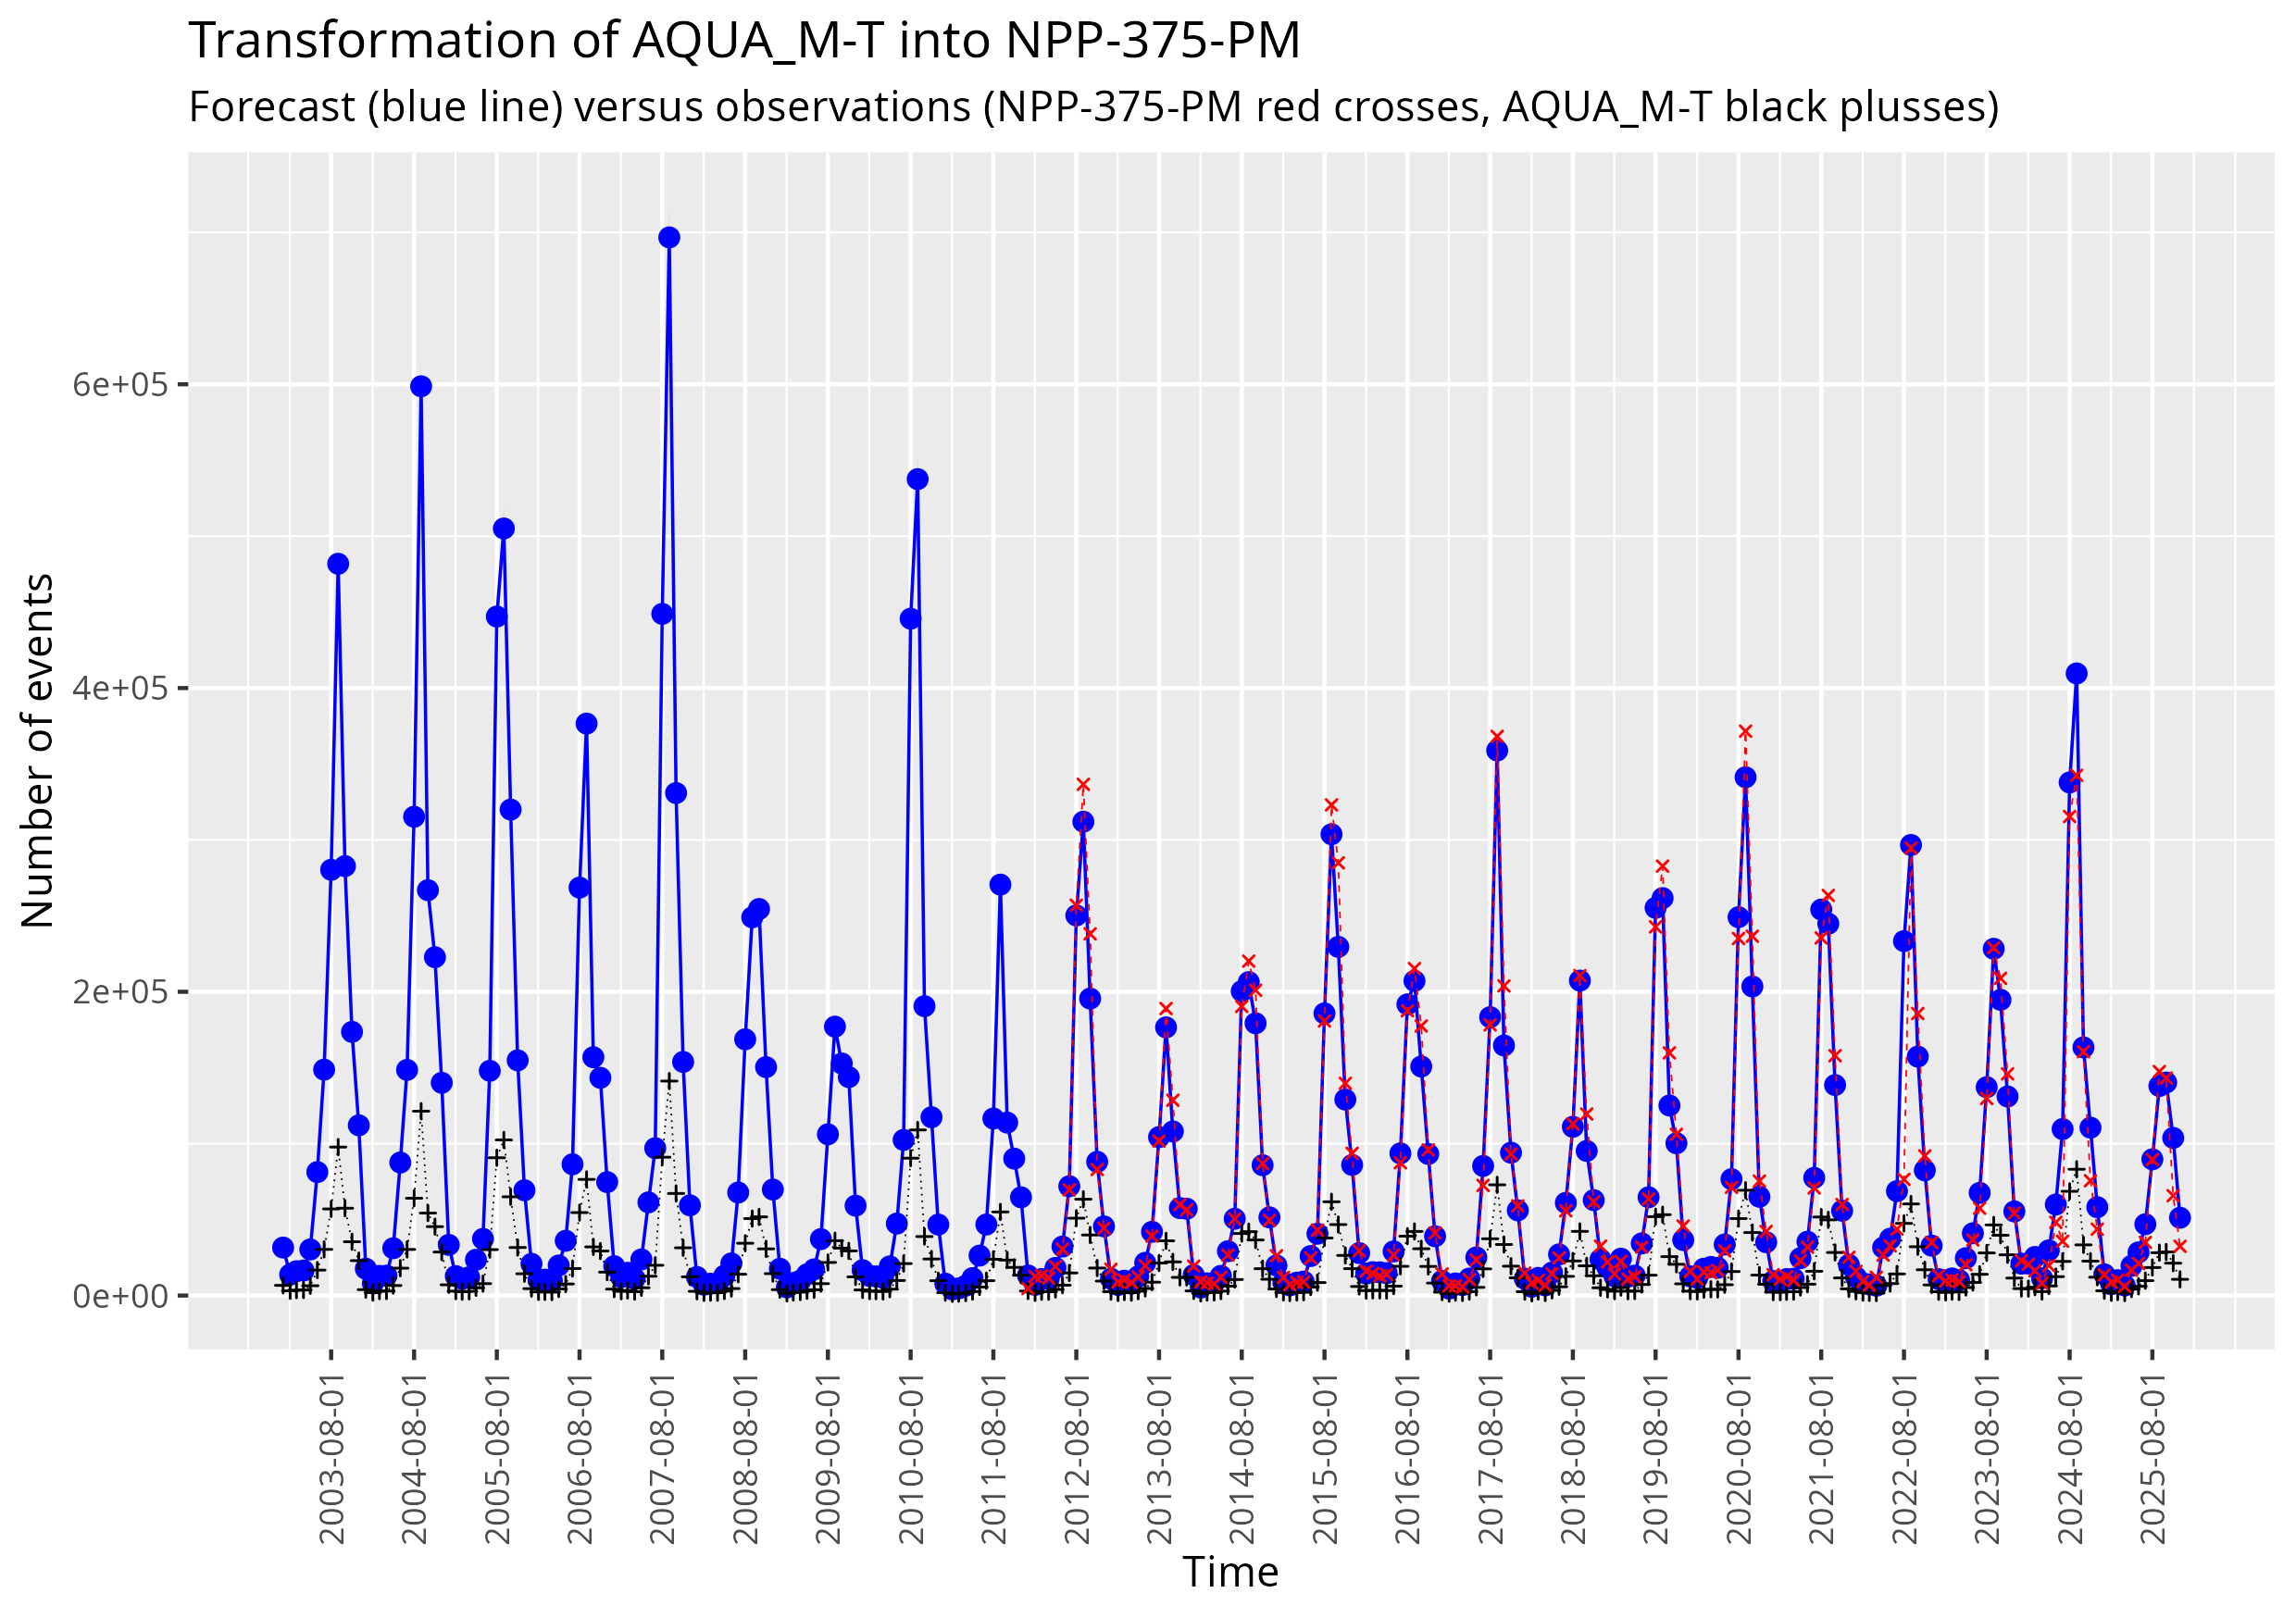
\includegraphics[scale=0.5]
    {figures/plot_forecast_01_NPP-375-PM_along_AQUA_M-T.png}
  \end{figure}
\end{frame}

\begin{frame}
  \frametitle{Stretch match AQUA\_M-T to match NOAA-12 (month-by-month)}
  \begin{figure}
    \centering
    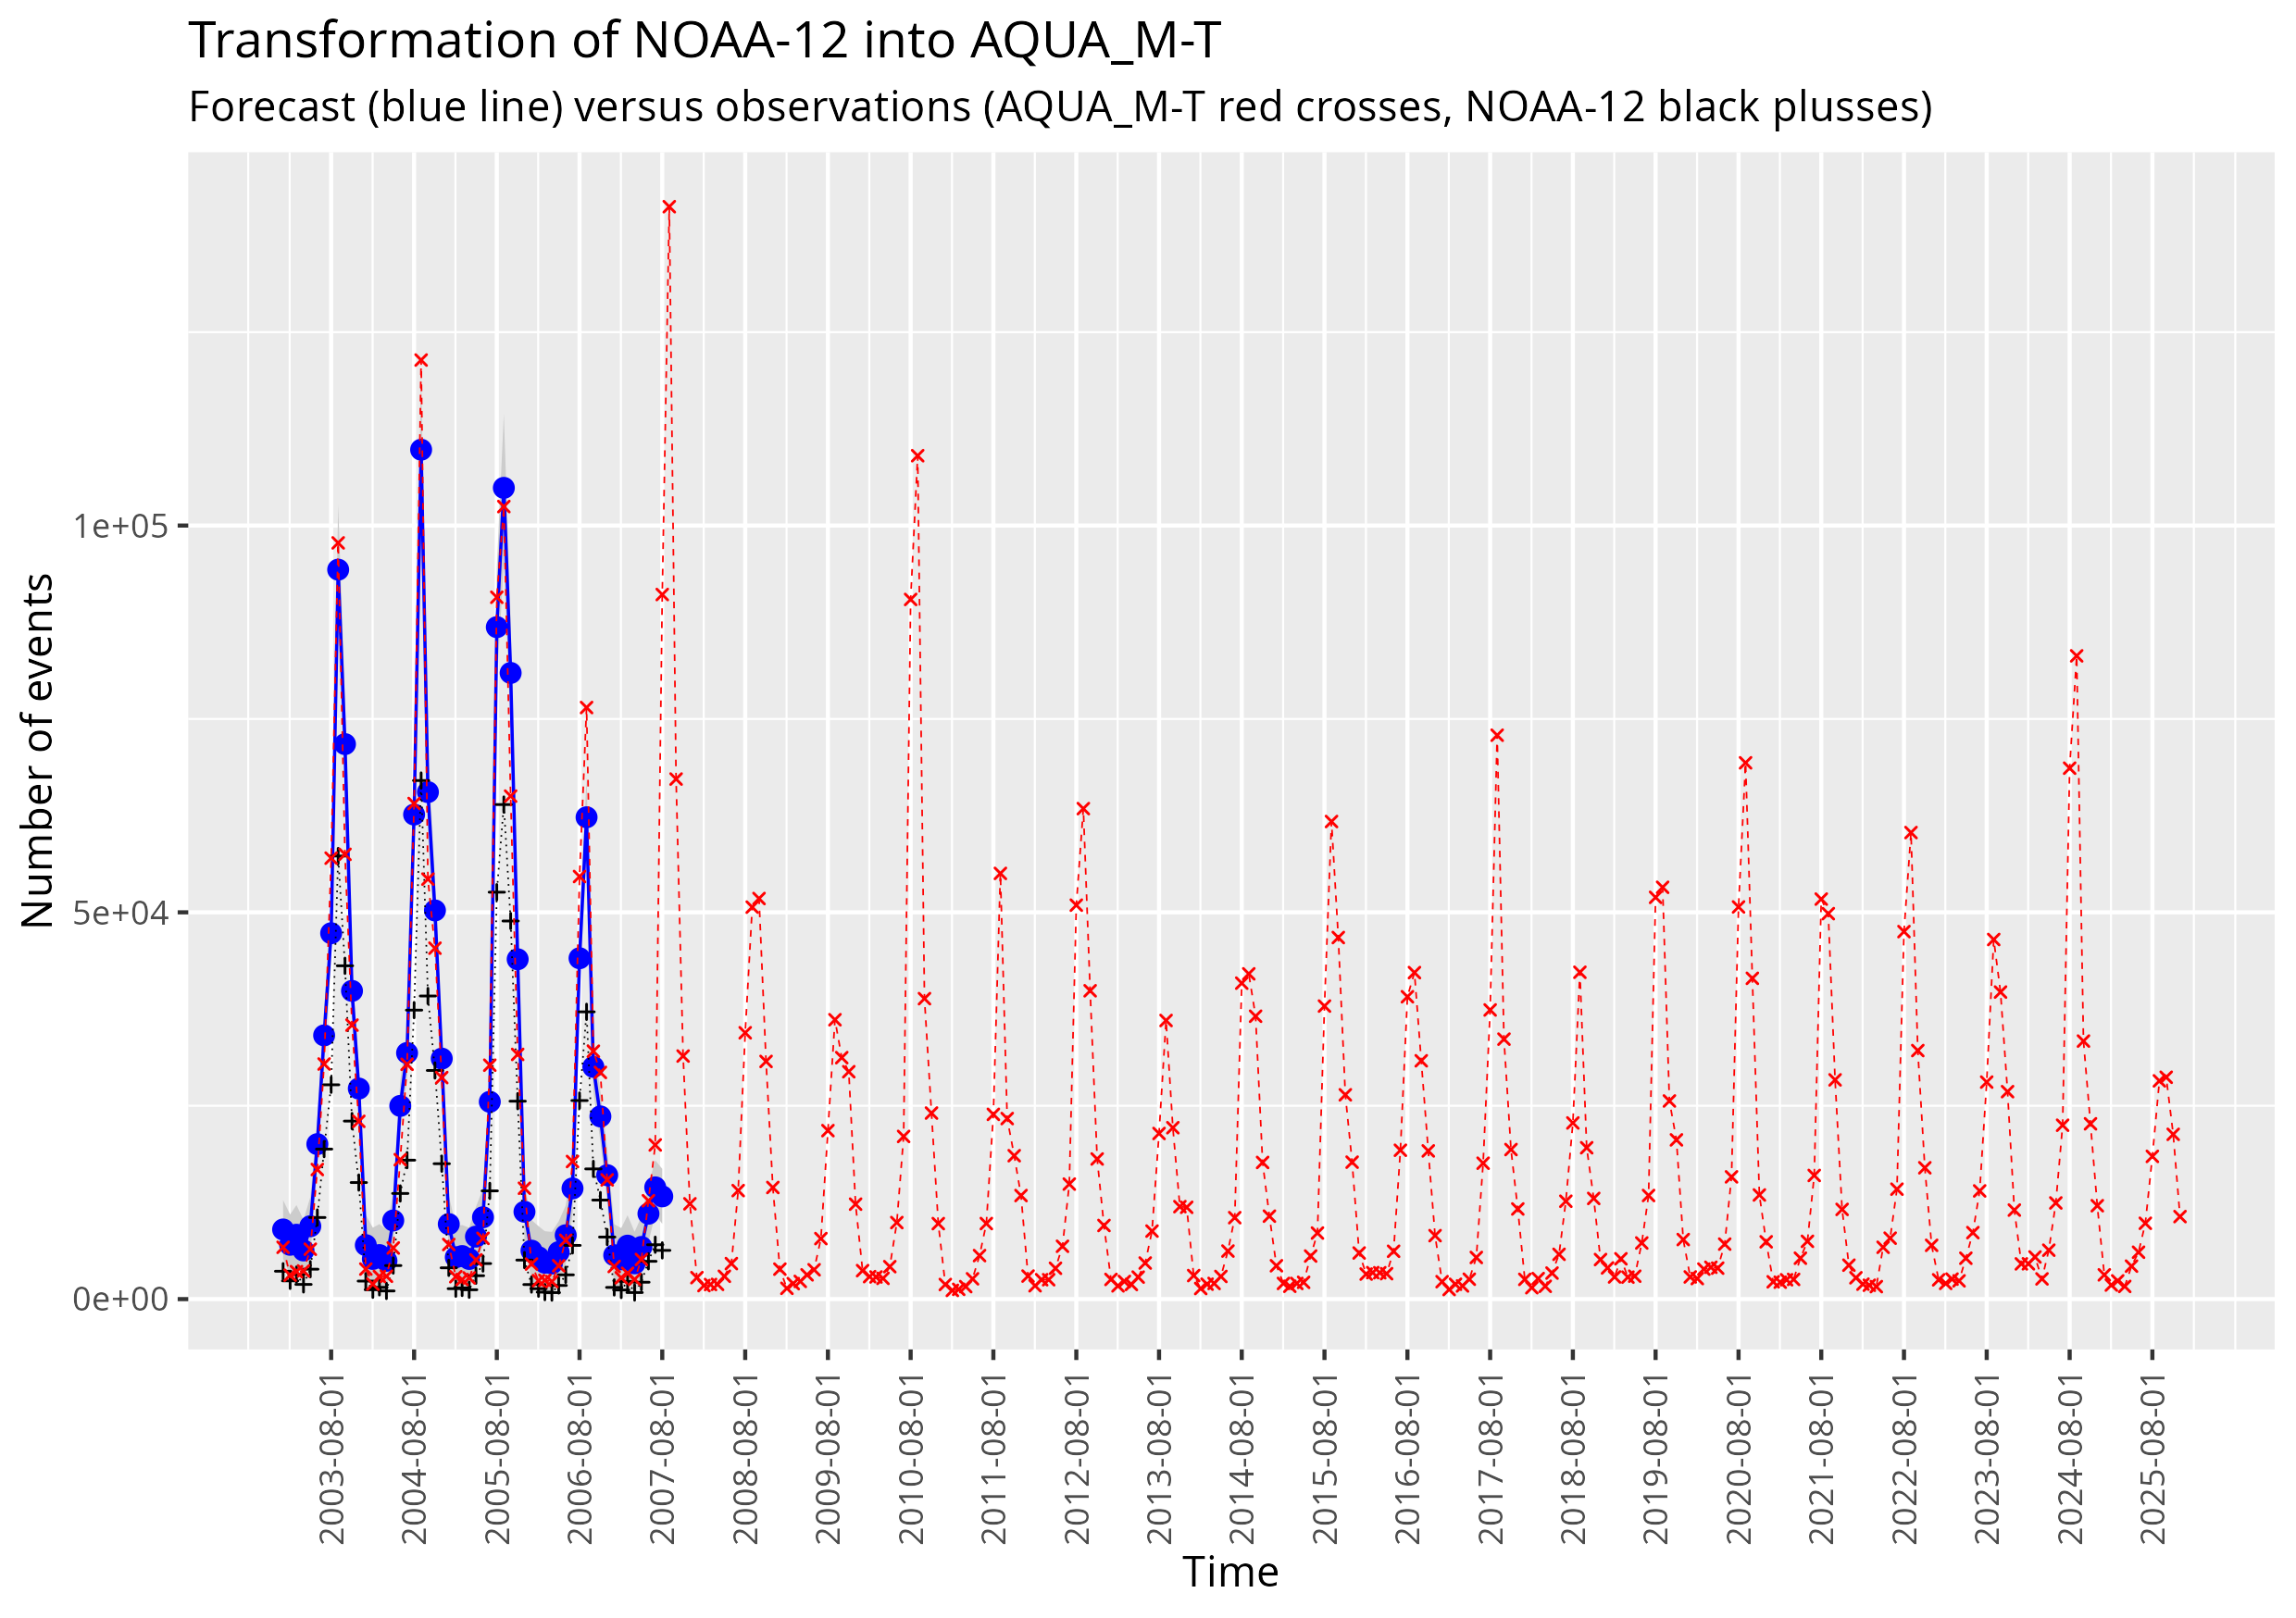
\includegraphics[scale=0.5]
    {figures/plot_forecast_01_AQUA_M-T_along_NOAA-12.png}
  \end{figure}
\end{frame}

\begin{frame}
  \frametitle{Stretch match AQUA\_M-T to match NPP-375-PM (month-by-month)}
  \begin{figure}
    \centering
    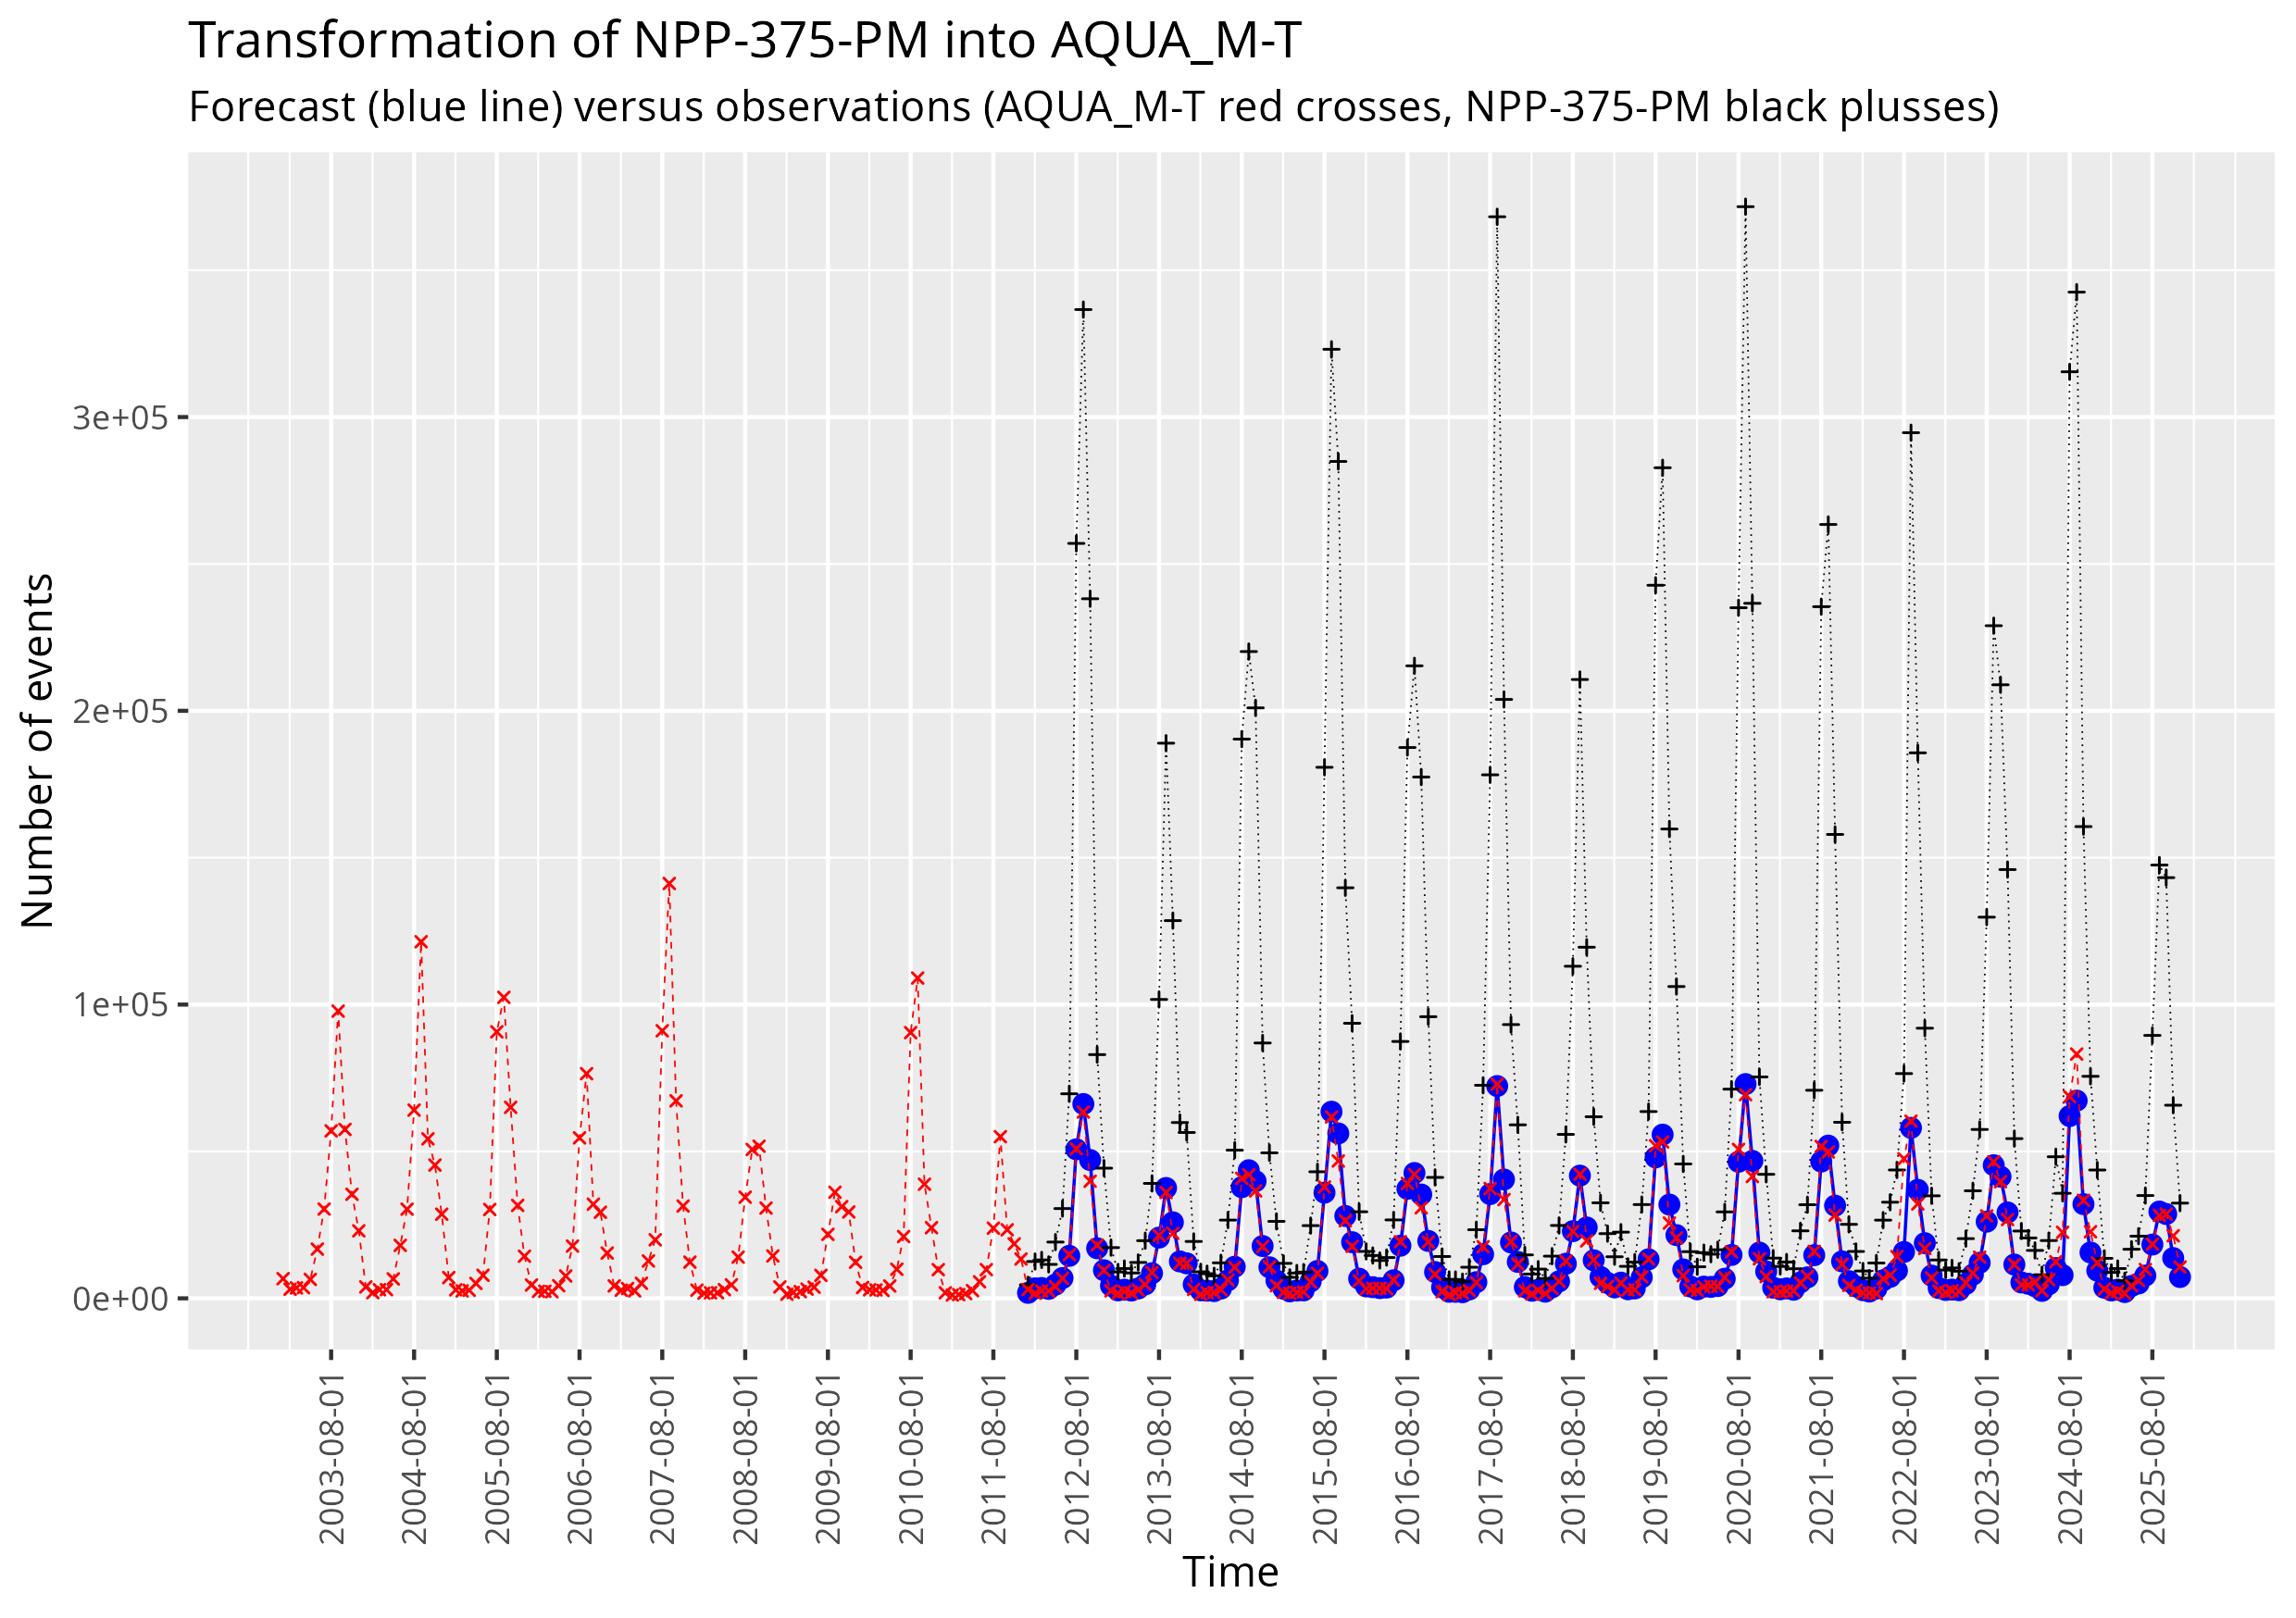
\includegraphics[scale=0.5]
    {figures/plot_forecast_01_AQUA_M-T_along_NPP-375-PM.png}
  \end{figure}
\end{frame}

\begin{frame}
  \frametitle{Stretch match NPP-375D to match NPP-375-PM (month-by-month)}
  \begin{figure}
    \centering
    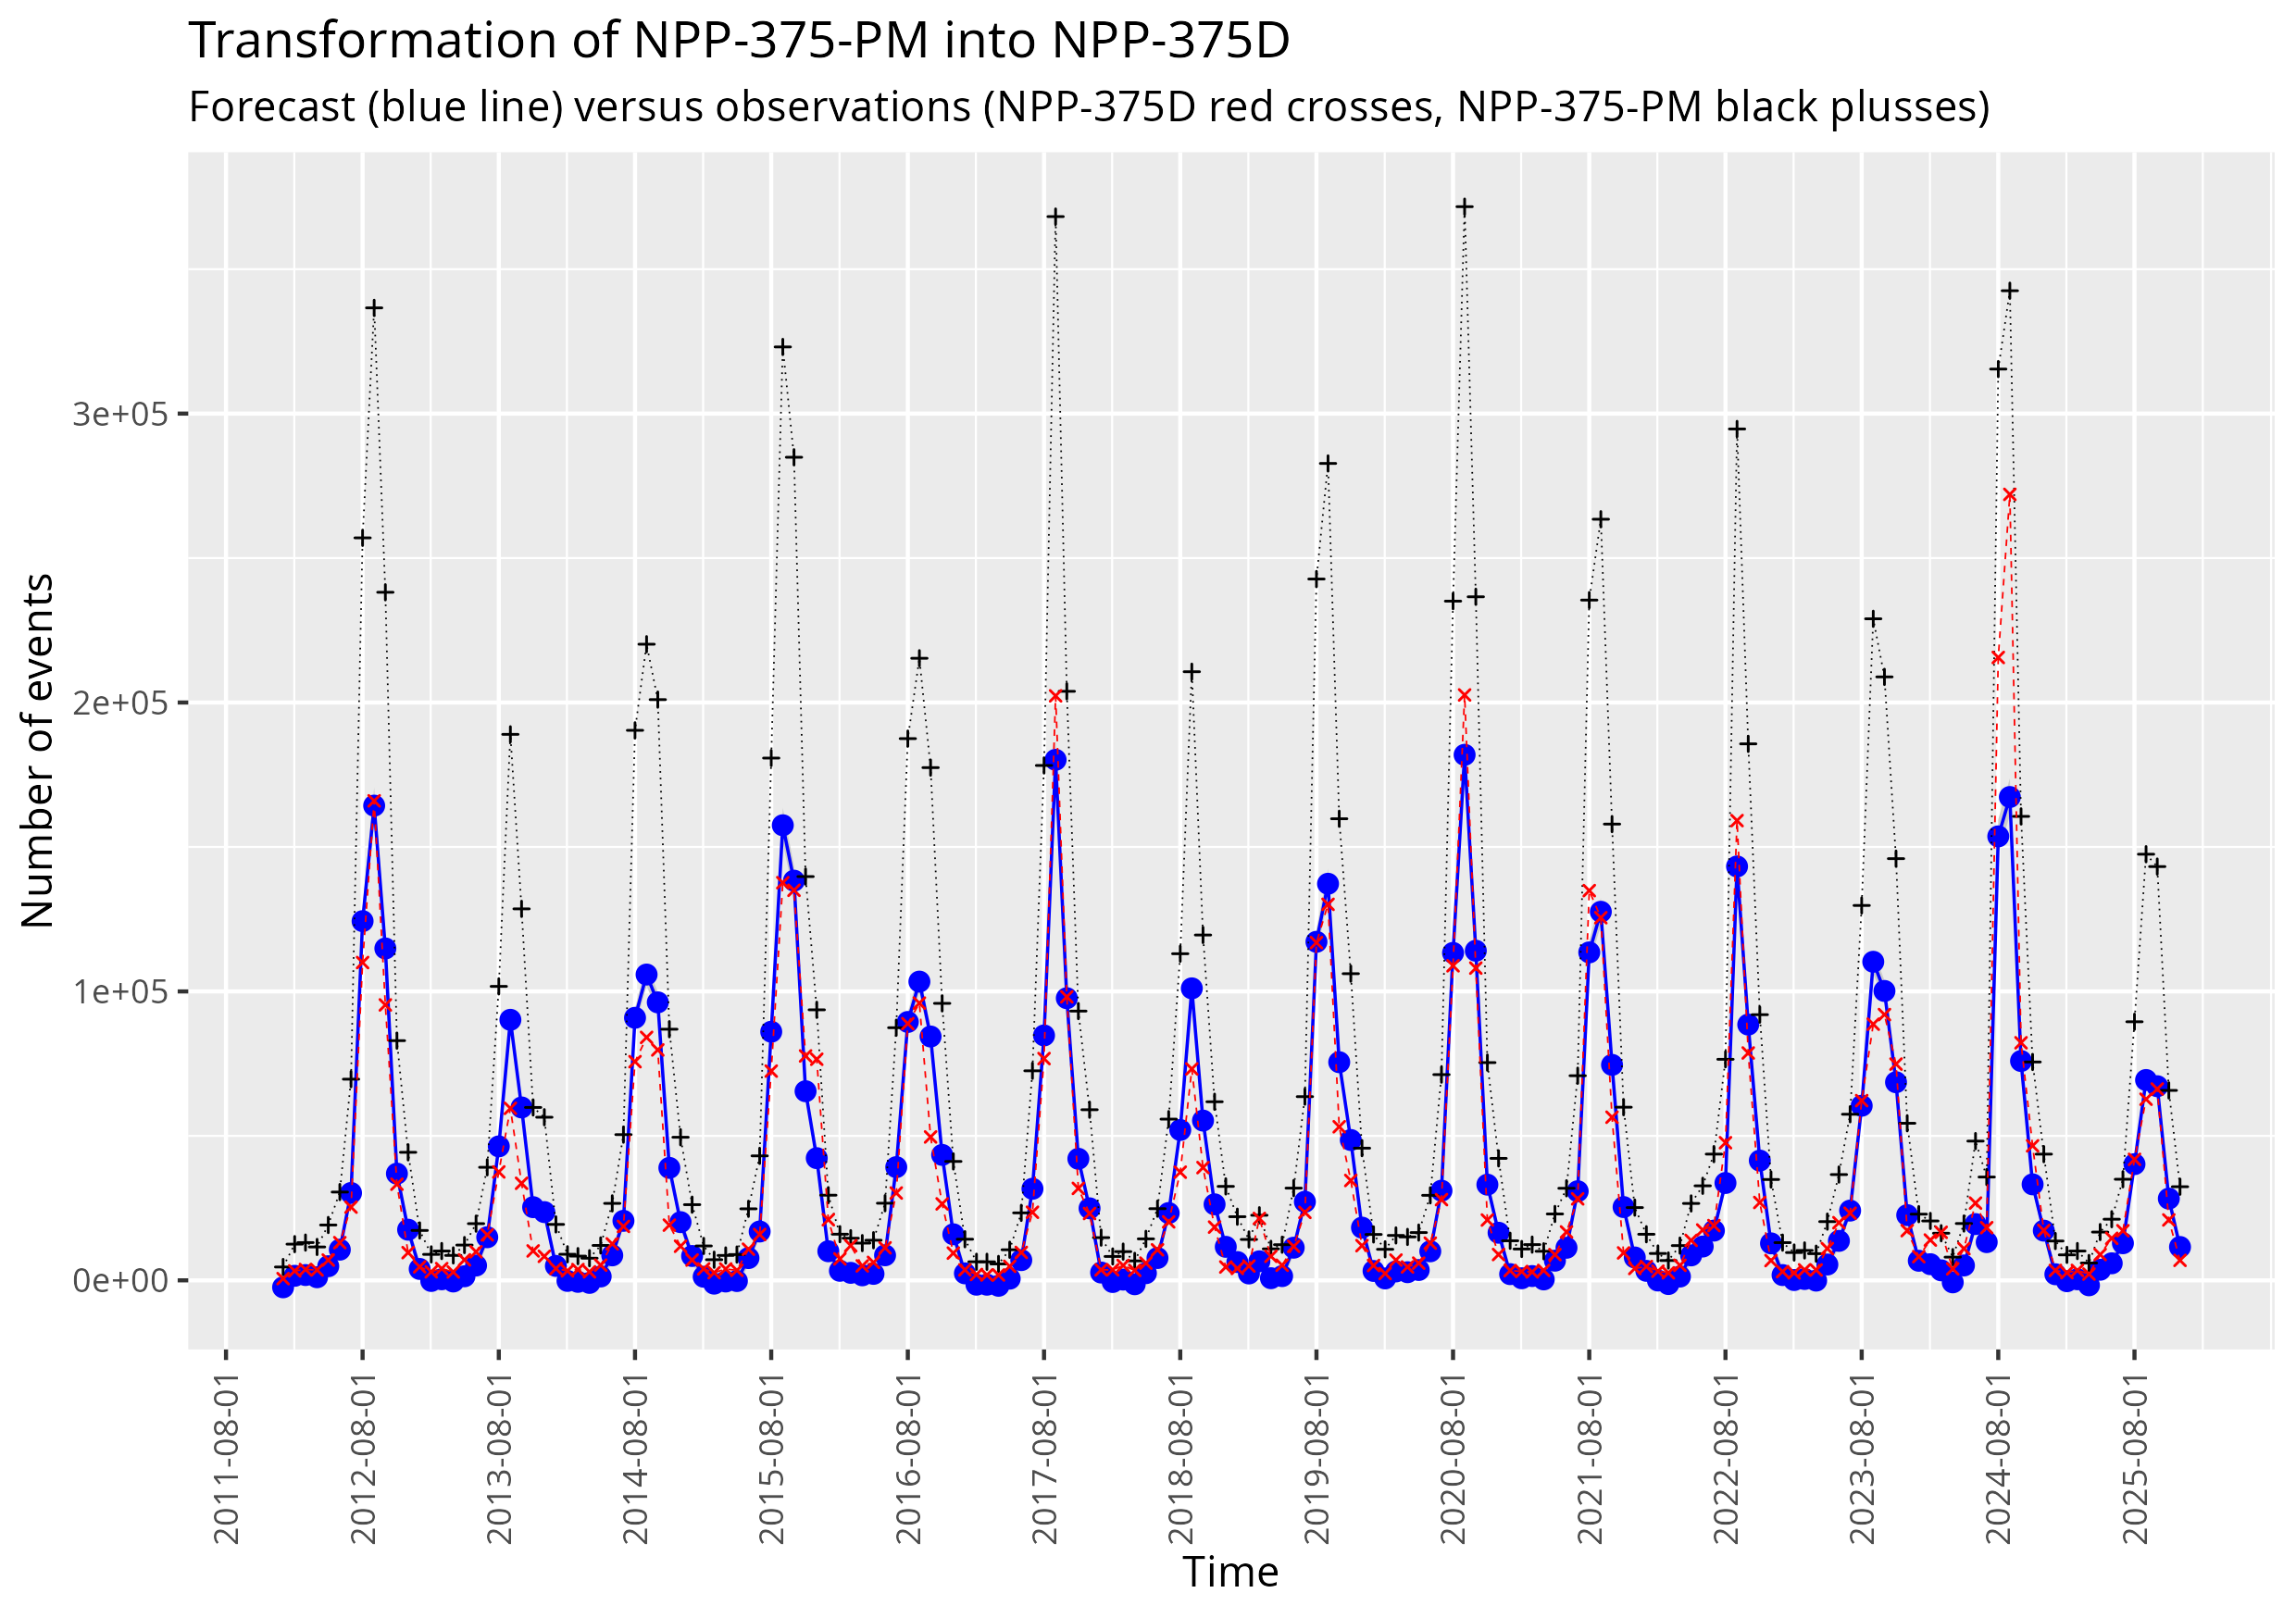
\includegraphics[scale=0.5]
    {figures/plot_forecast_01_NPP-375D_along_NPP-375-PM.png}
  \end{figure}
\end{frame}

\begin{frame}
  \frametitle{Stretch match AQUA\_M-T to match NPP-375D (month-by-month)}
  \begin{figure}
    \centering
    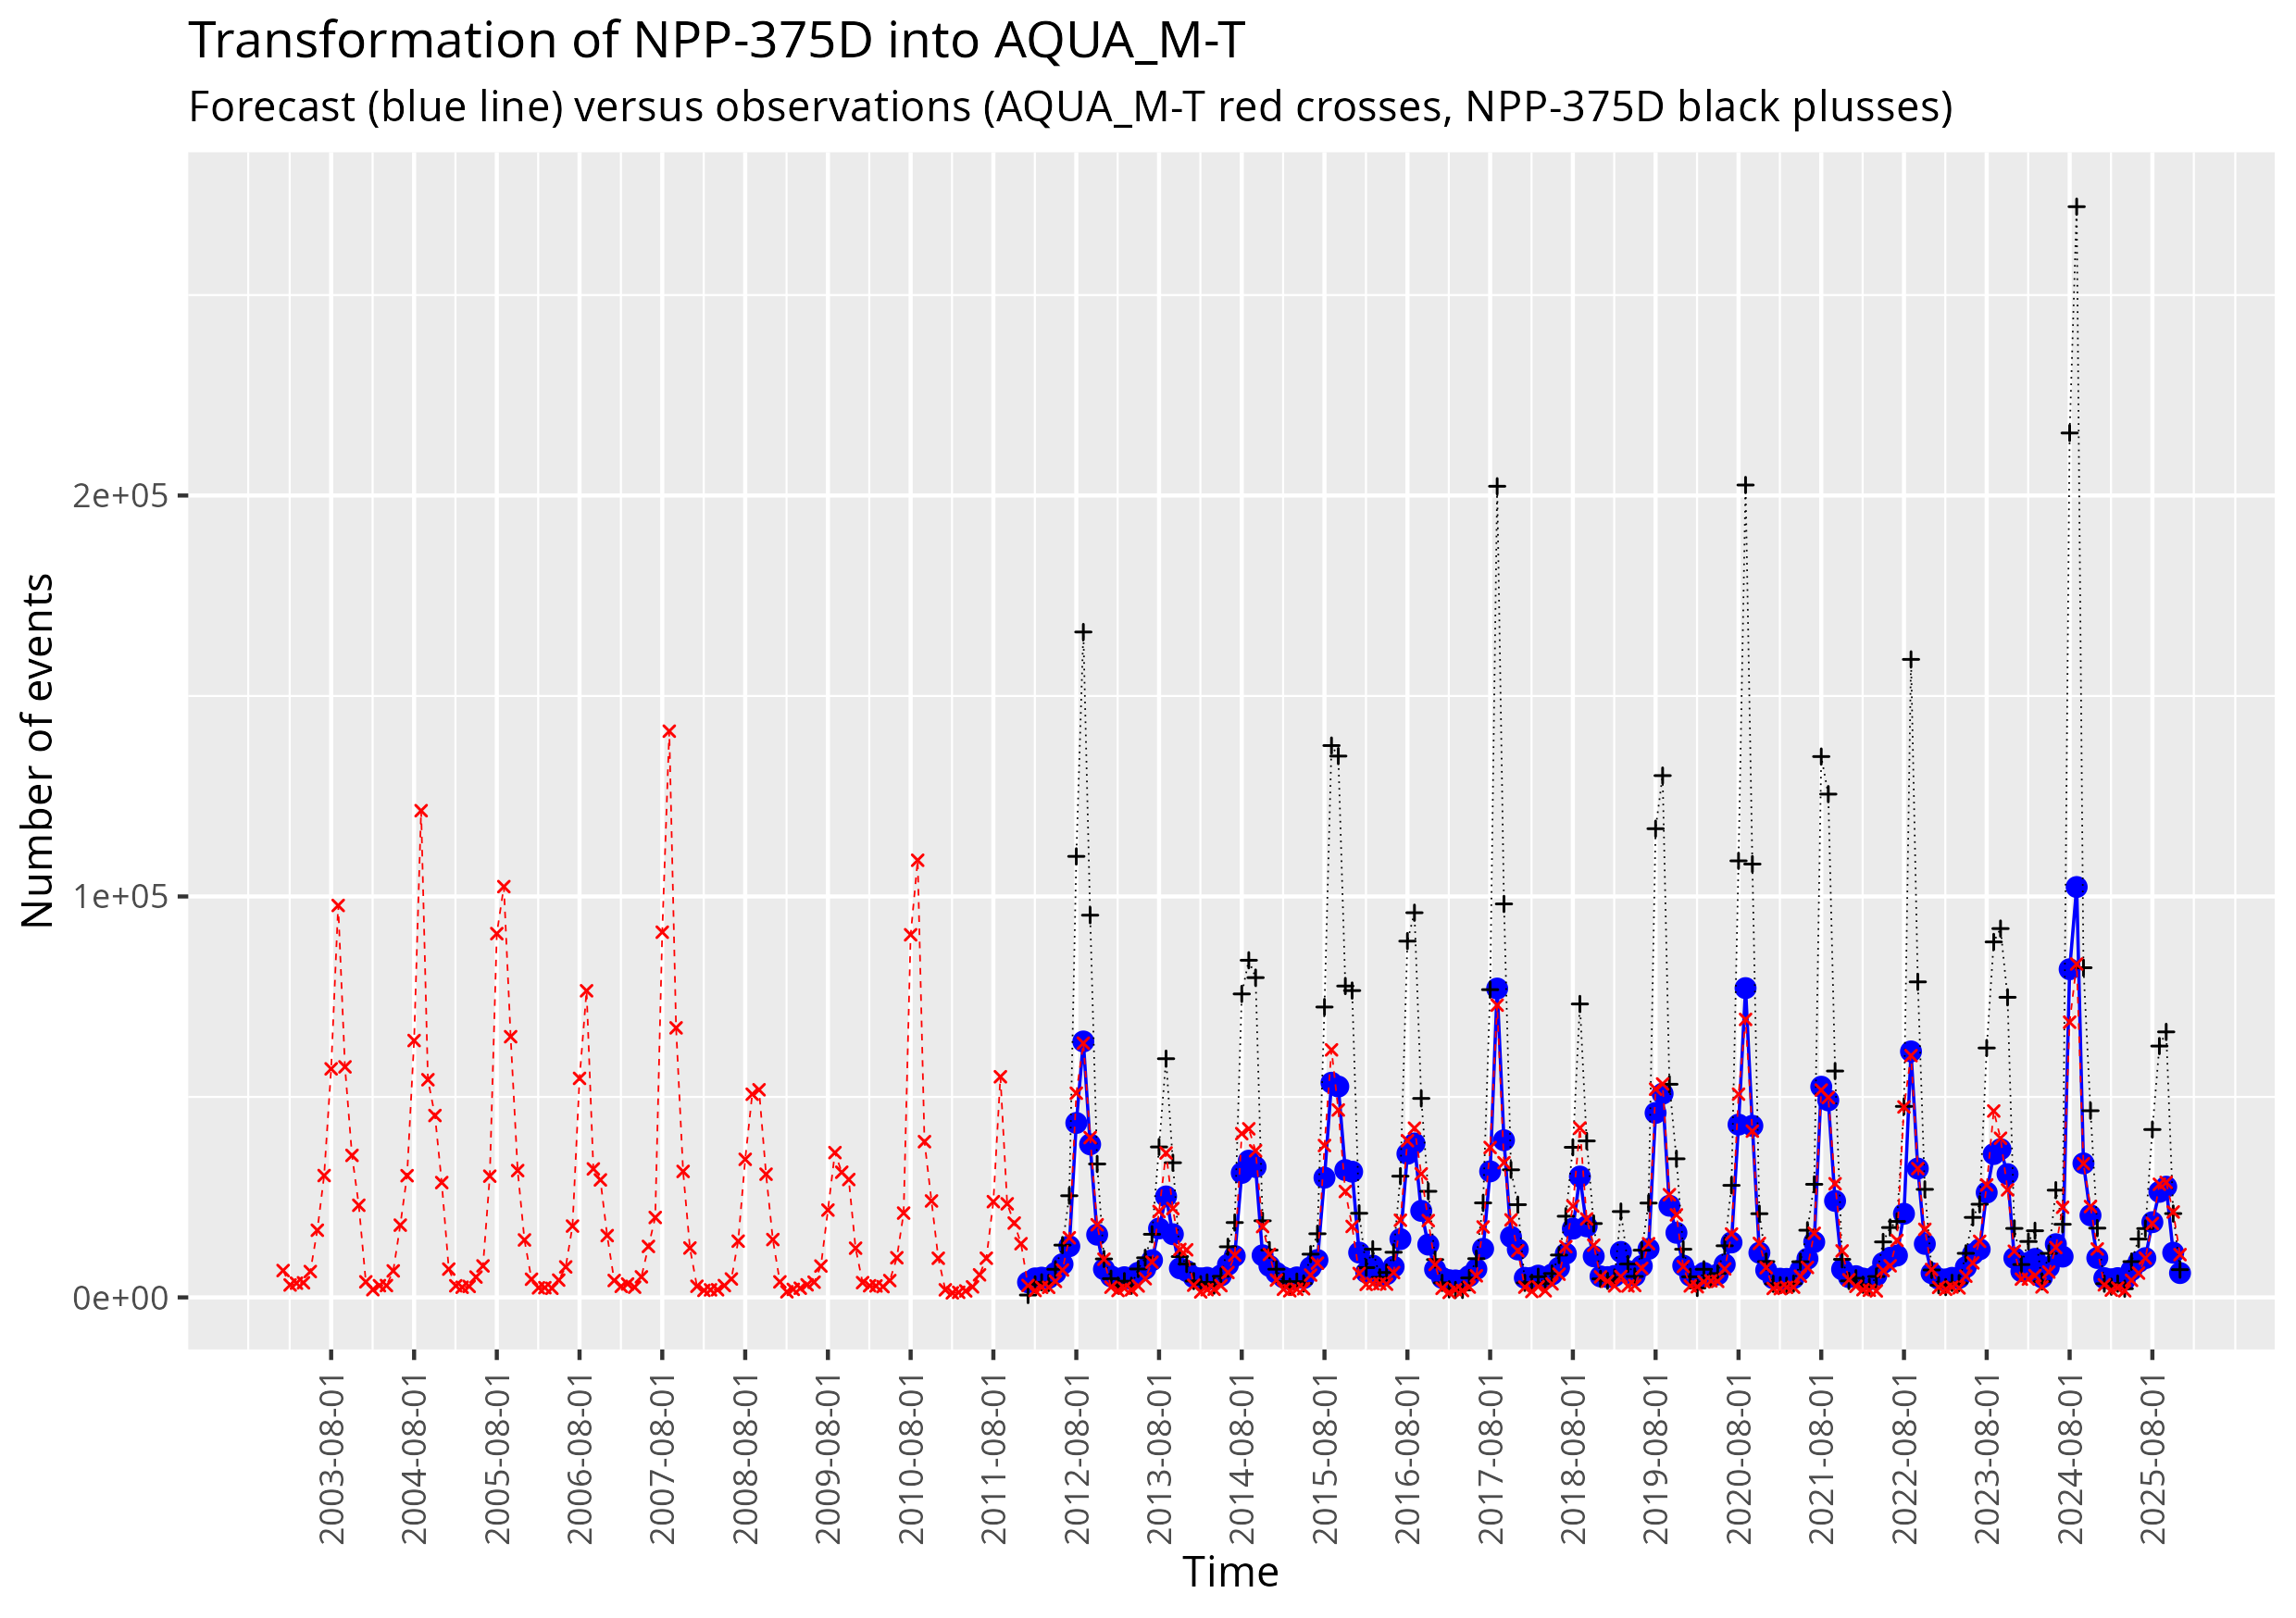
\includegraphics[scale=0.5]
    {figures/plot_forecast_01_AQUA_M-T_along_NPP-375D.png}
  \end{figure}
\end{frame}

\begin{frame}
  \frametitle{Stretch match NPP-375-PM to match NPP-375D (month-by-month)}
  \begin{figure}
    \centering
    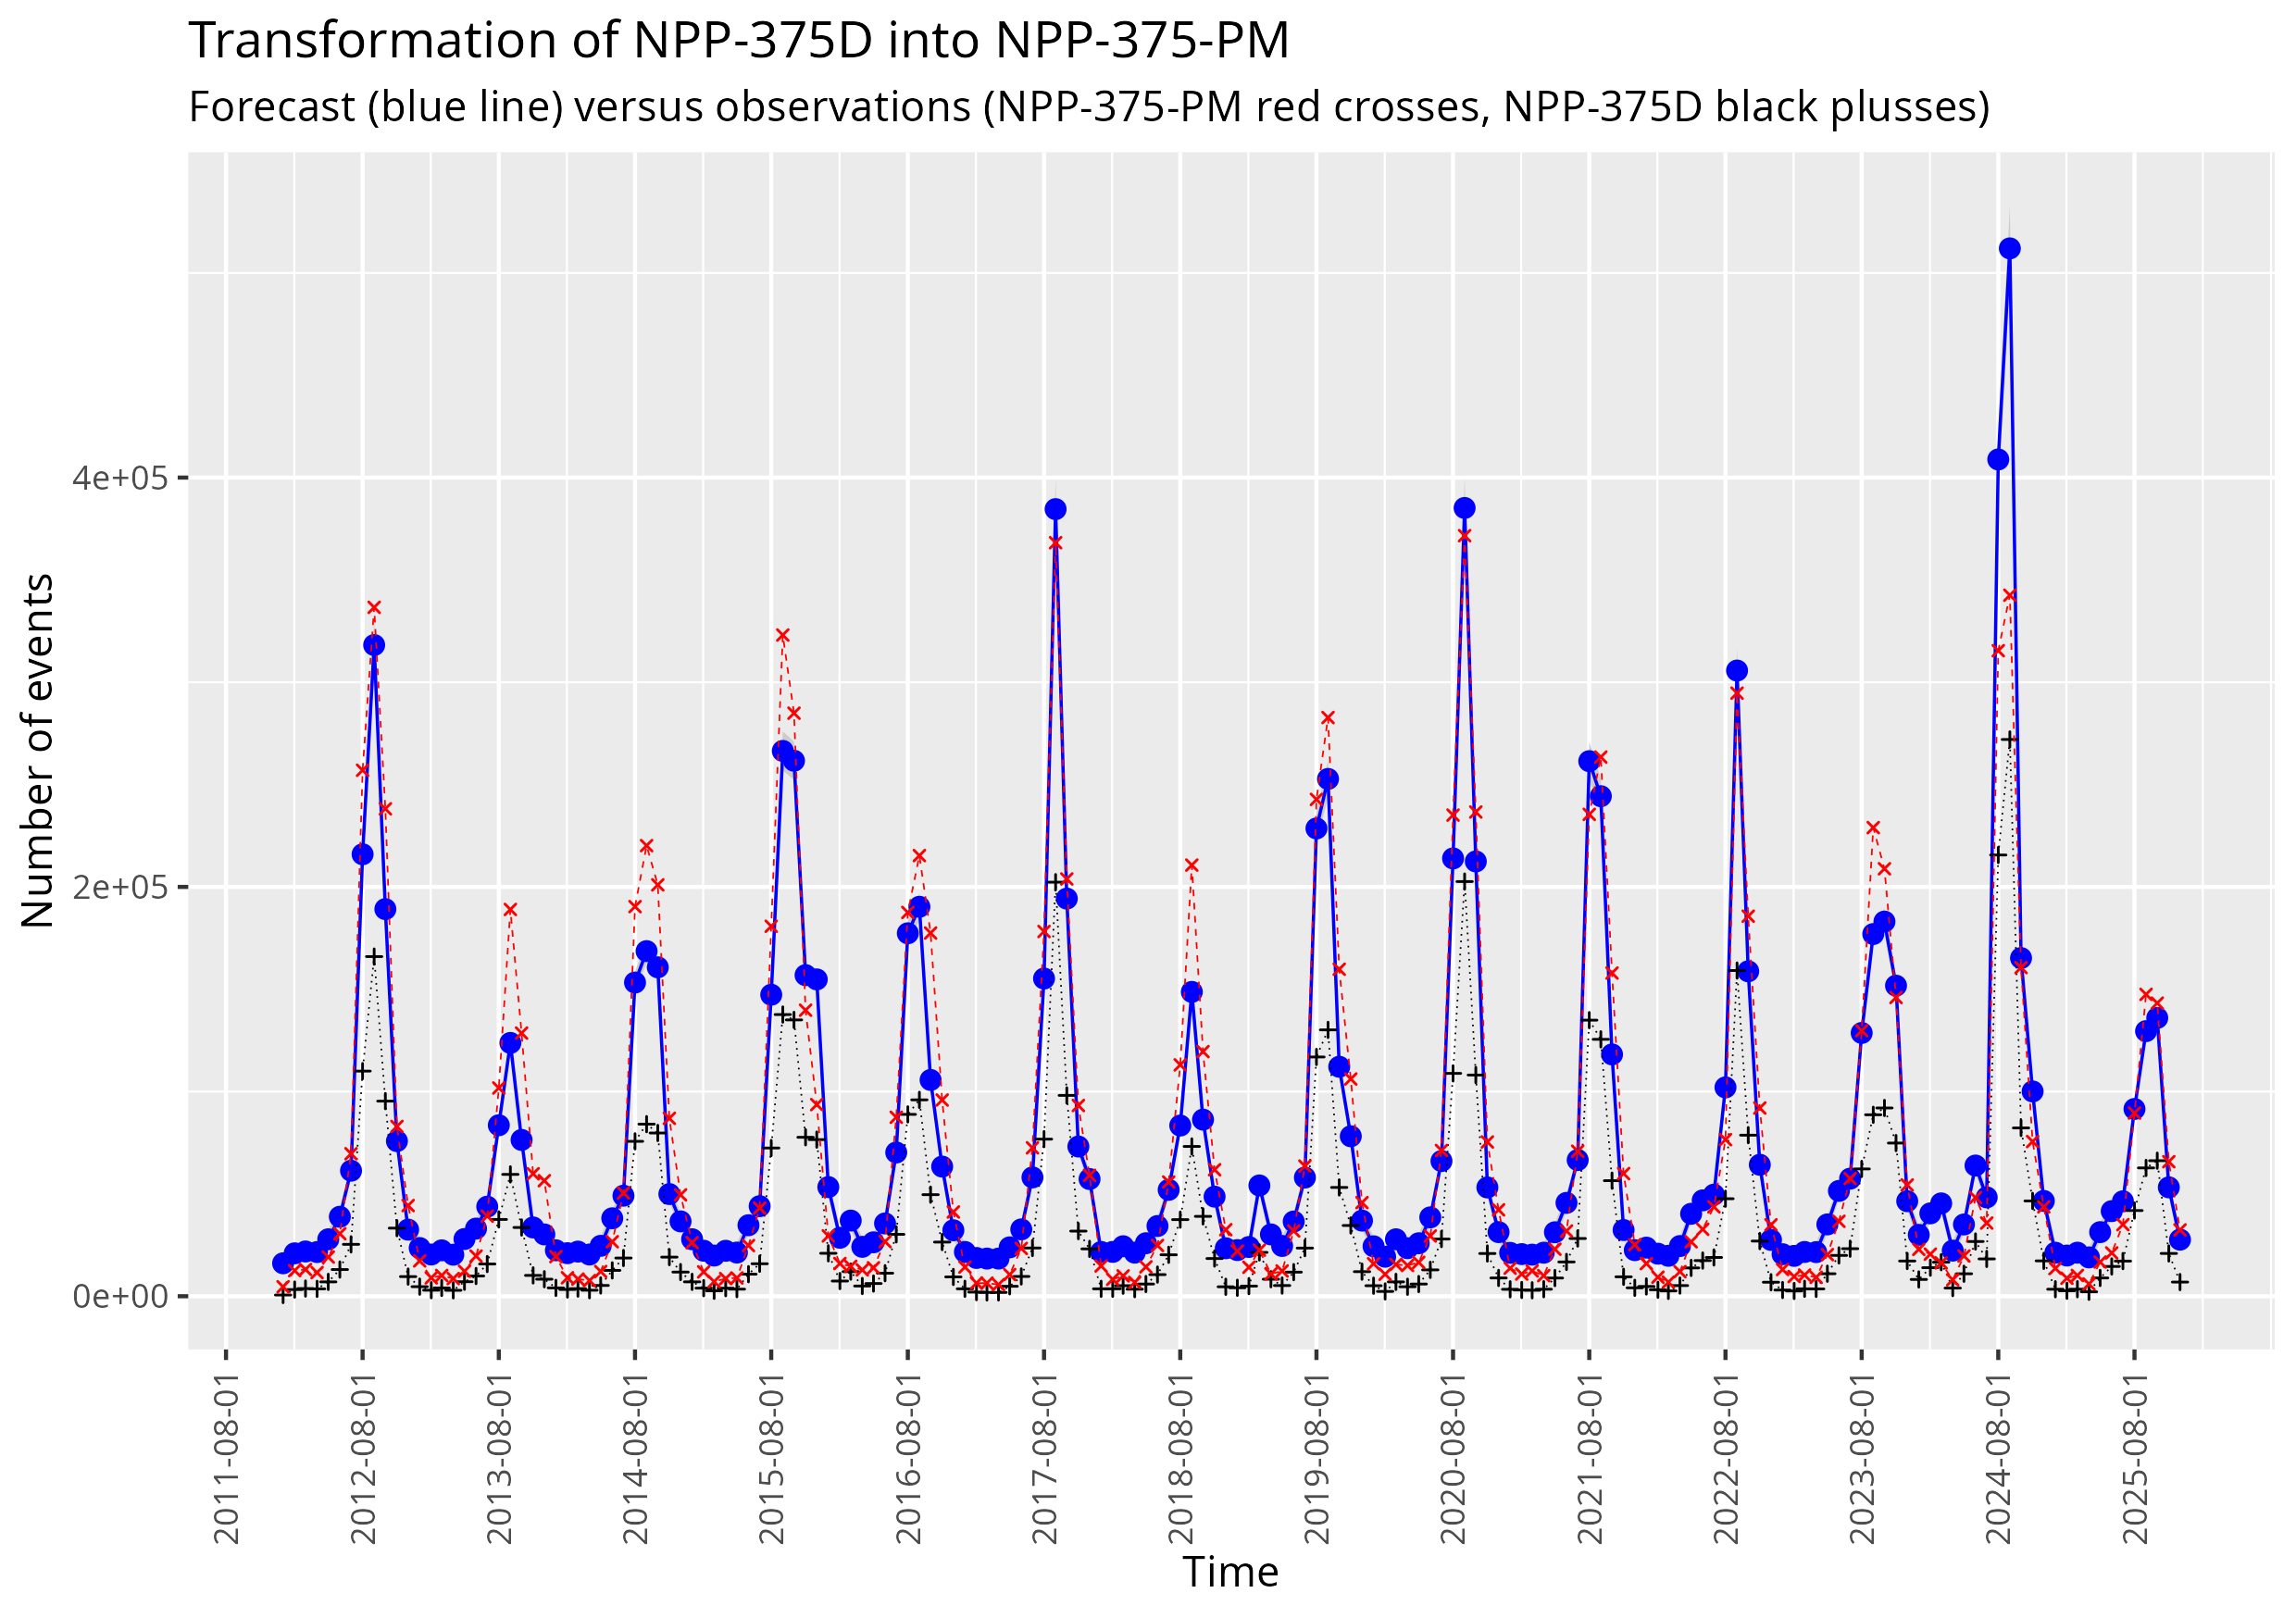
\includegraphics[scale=0.5]
    {figures/plot_forecast_01_NPP-375-PM_along_NPP-375D.png}
  \end{figure}
\end{frame}

\subsection{Forecast differences}

\begin{frame}
  Forecast differences between Queimadas' 12 versus 1 month method
\end{frame}

\begin{frame}
  \frametitle{Forecast differences NOAA-12 vs. AQUA\_M-T}
  \begin{figure}
    \centering
    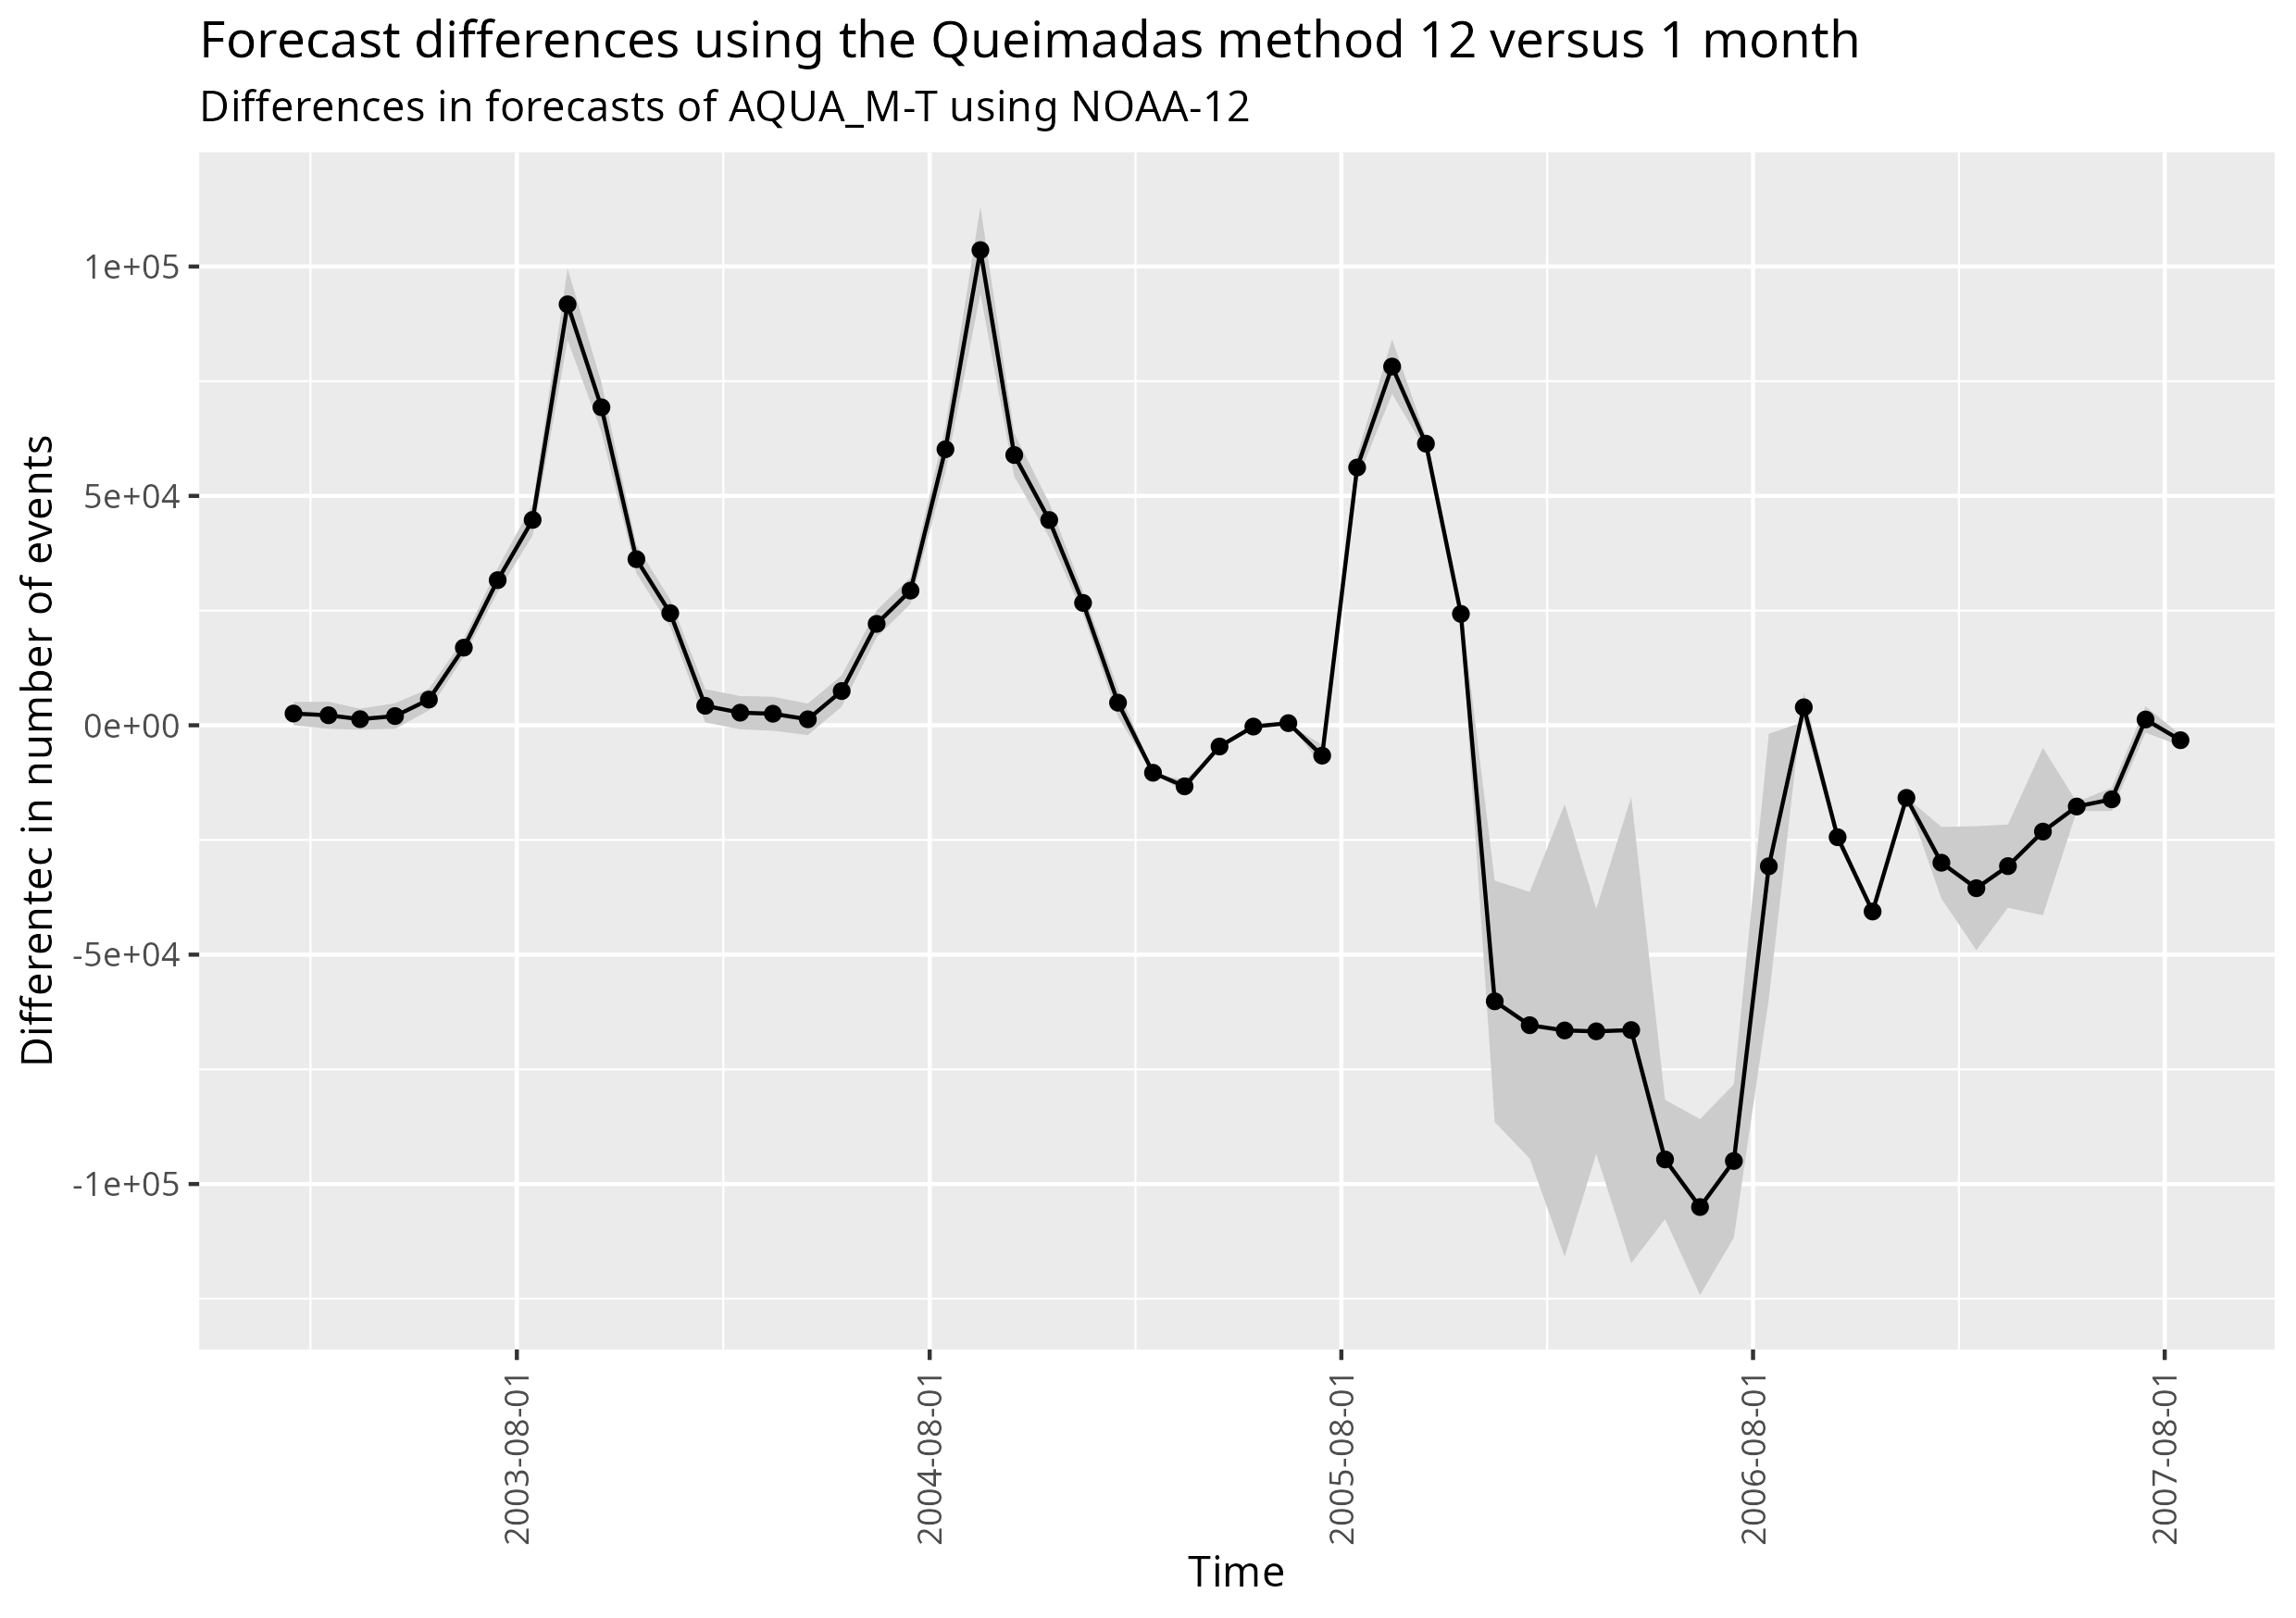
\includegraphics[scale=0.5]
    {figures/plot_forecast_differences_12_vs_1_AQUA_M-T_along_NOAA-12.png}
  \end{figure}
\end{frame}

\begin{frame}
  \frametitle{Forecast differences NPP-375D vs. AQUA\_M-T}
  \begin{figure}
    \centering
    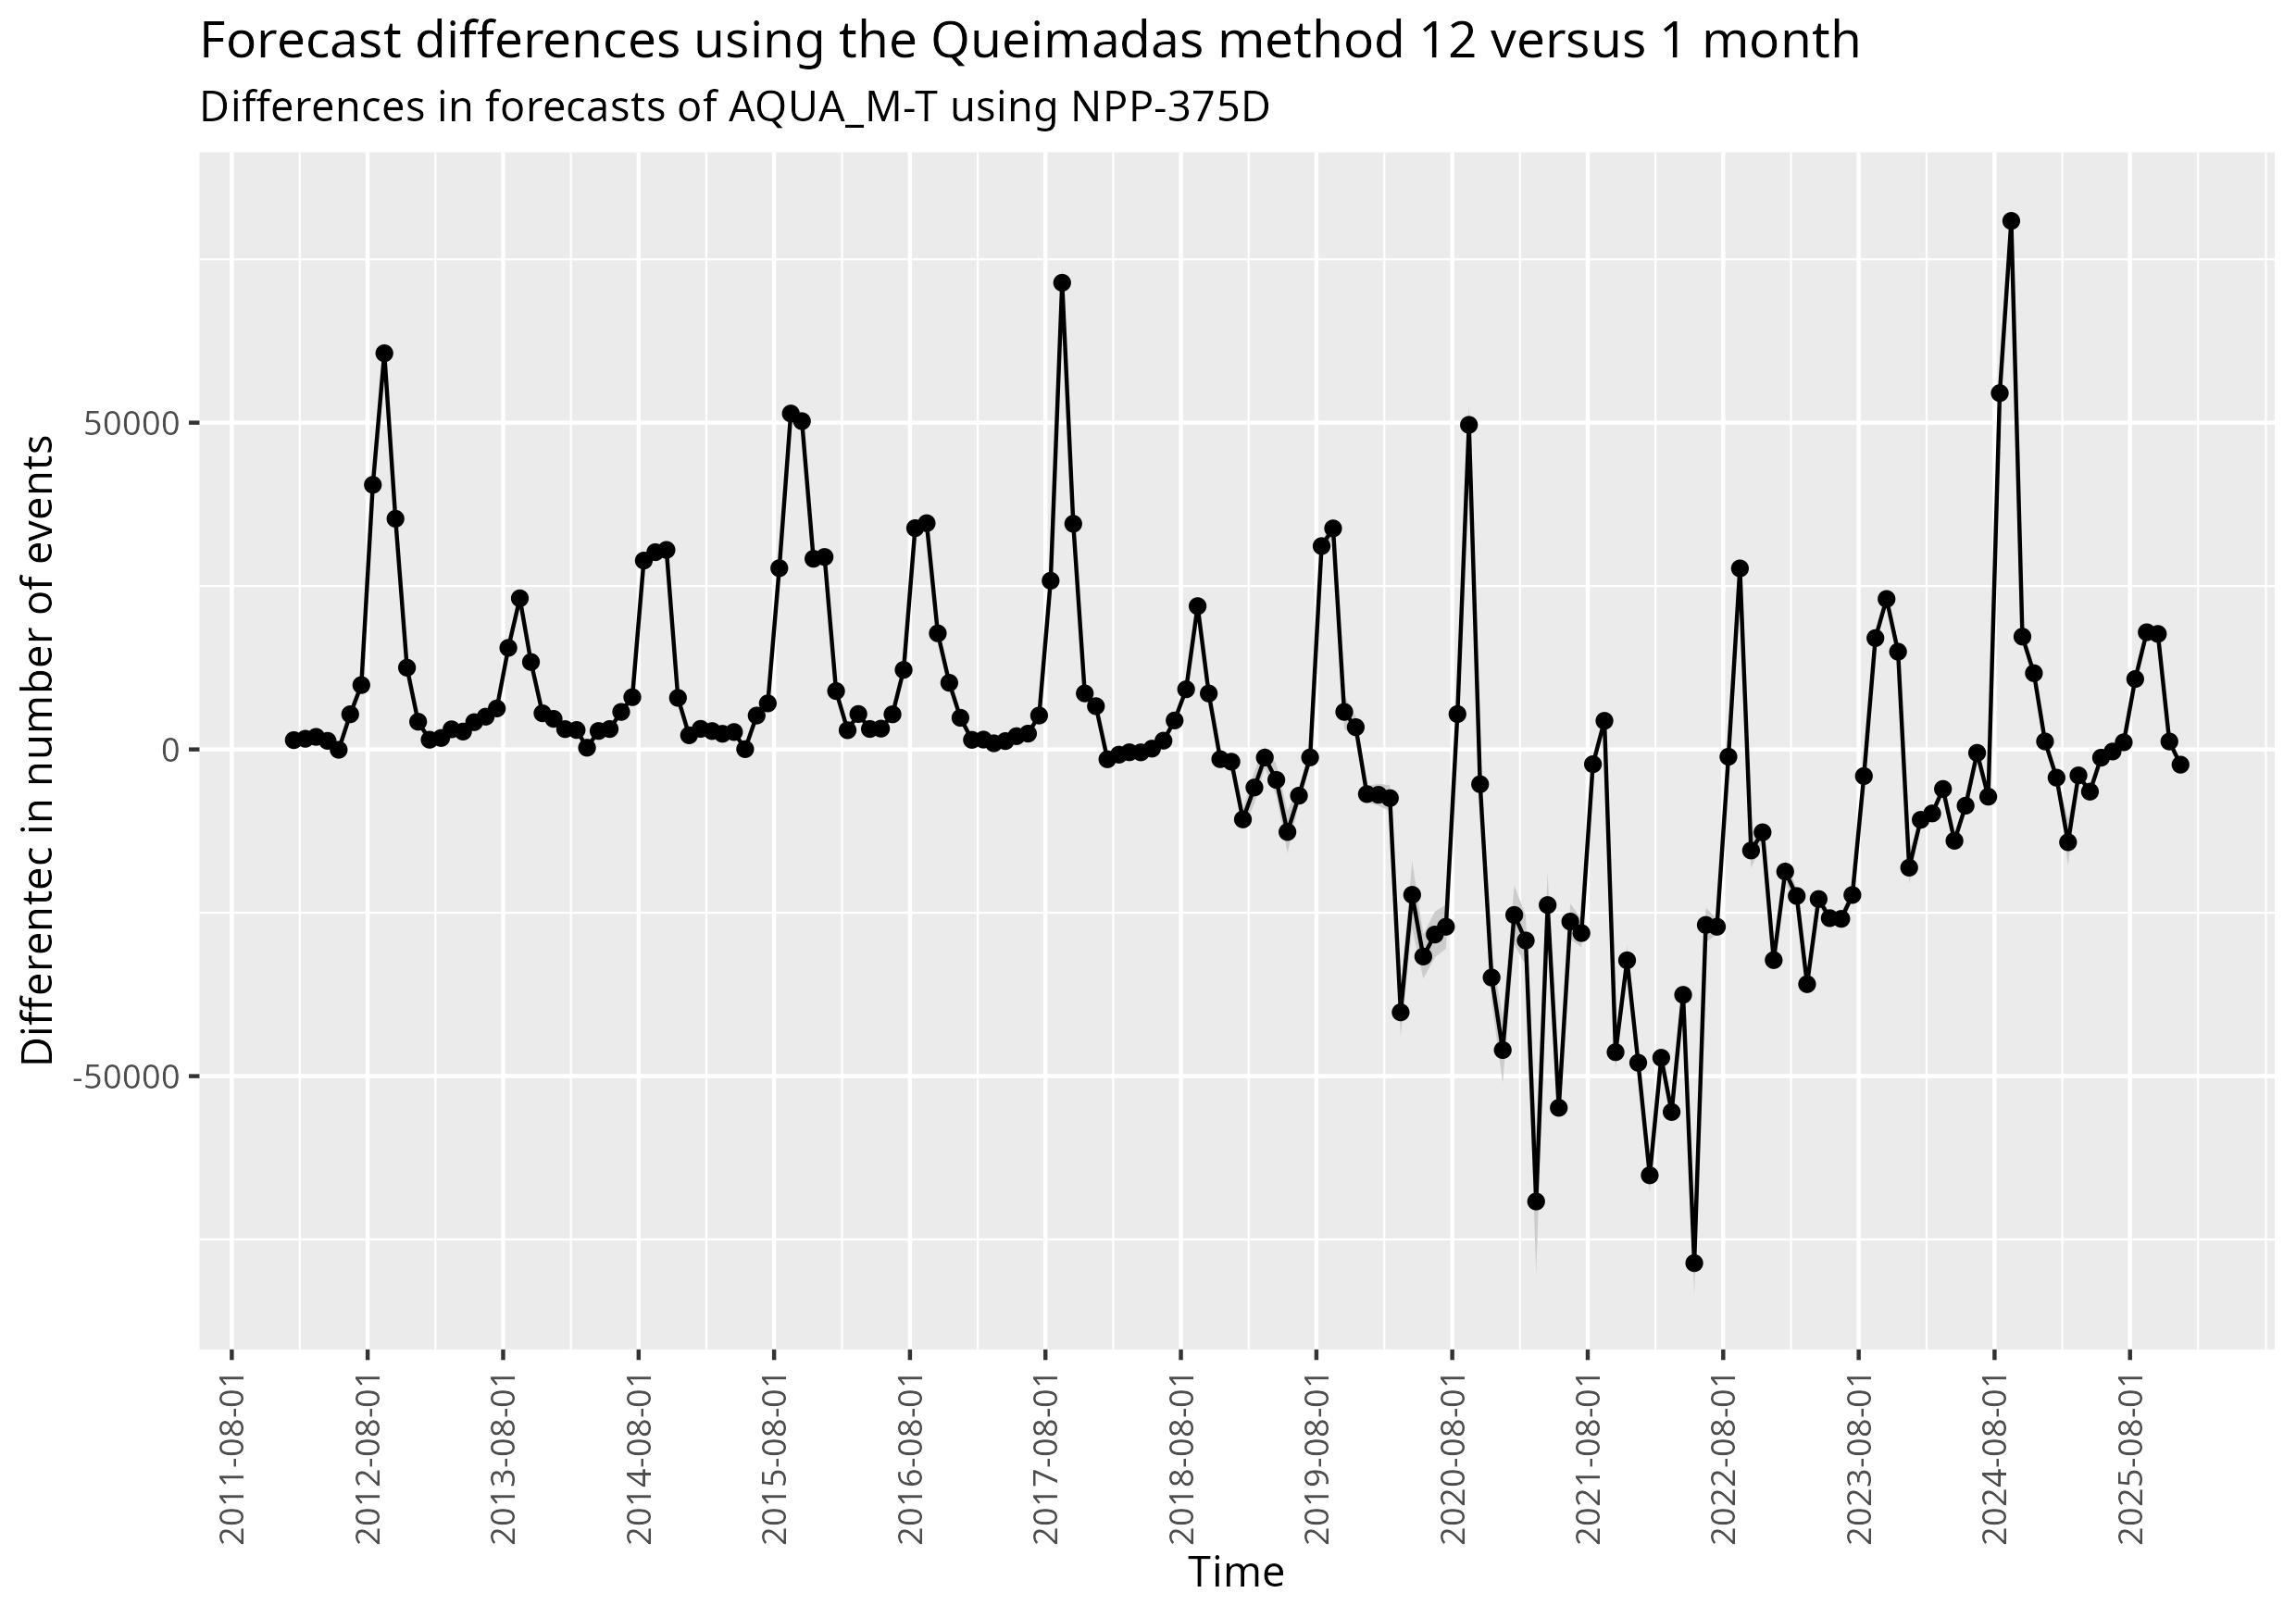
\includegraphics[scale=0.5]
    {figures/plot_forecast_differences_12_vs_1_AQUA_M-T_along_NPP-375D.png}
  \end{figure}
\end{frame}

\begin{frame}
  \frametitle{Forecast differences NPP-375PM vs. AQUA\_M-T}
  \begin{figure}
    \centering
    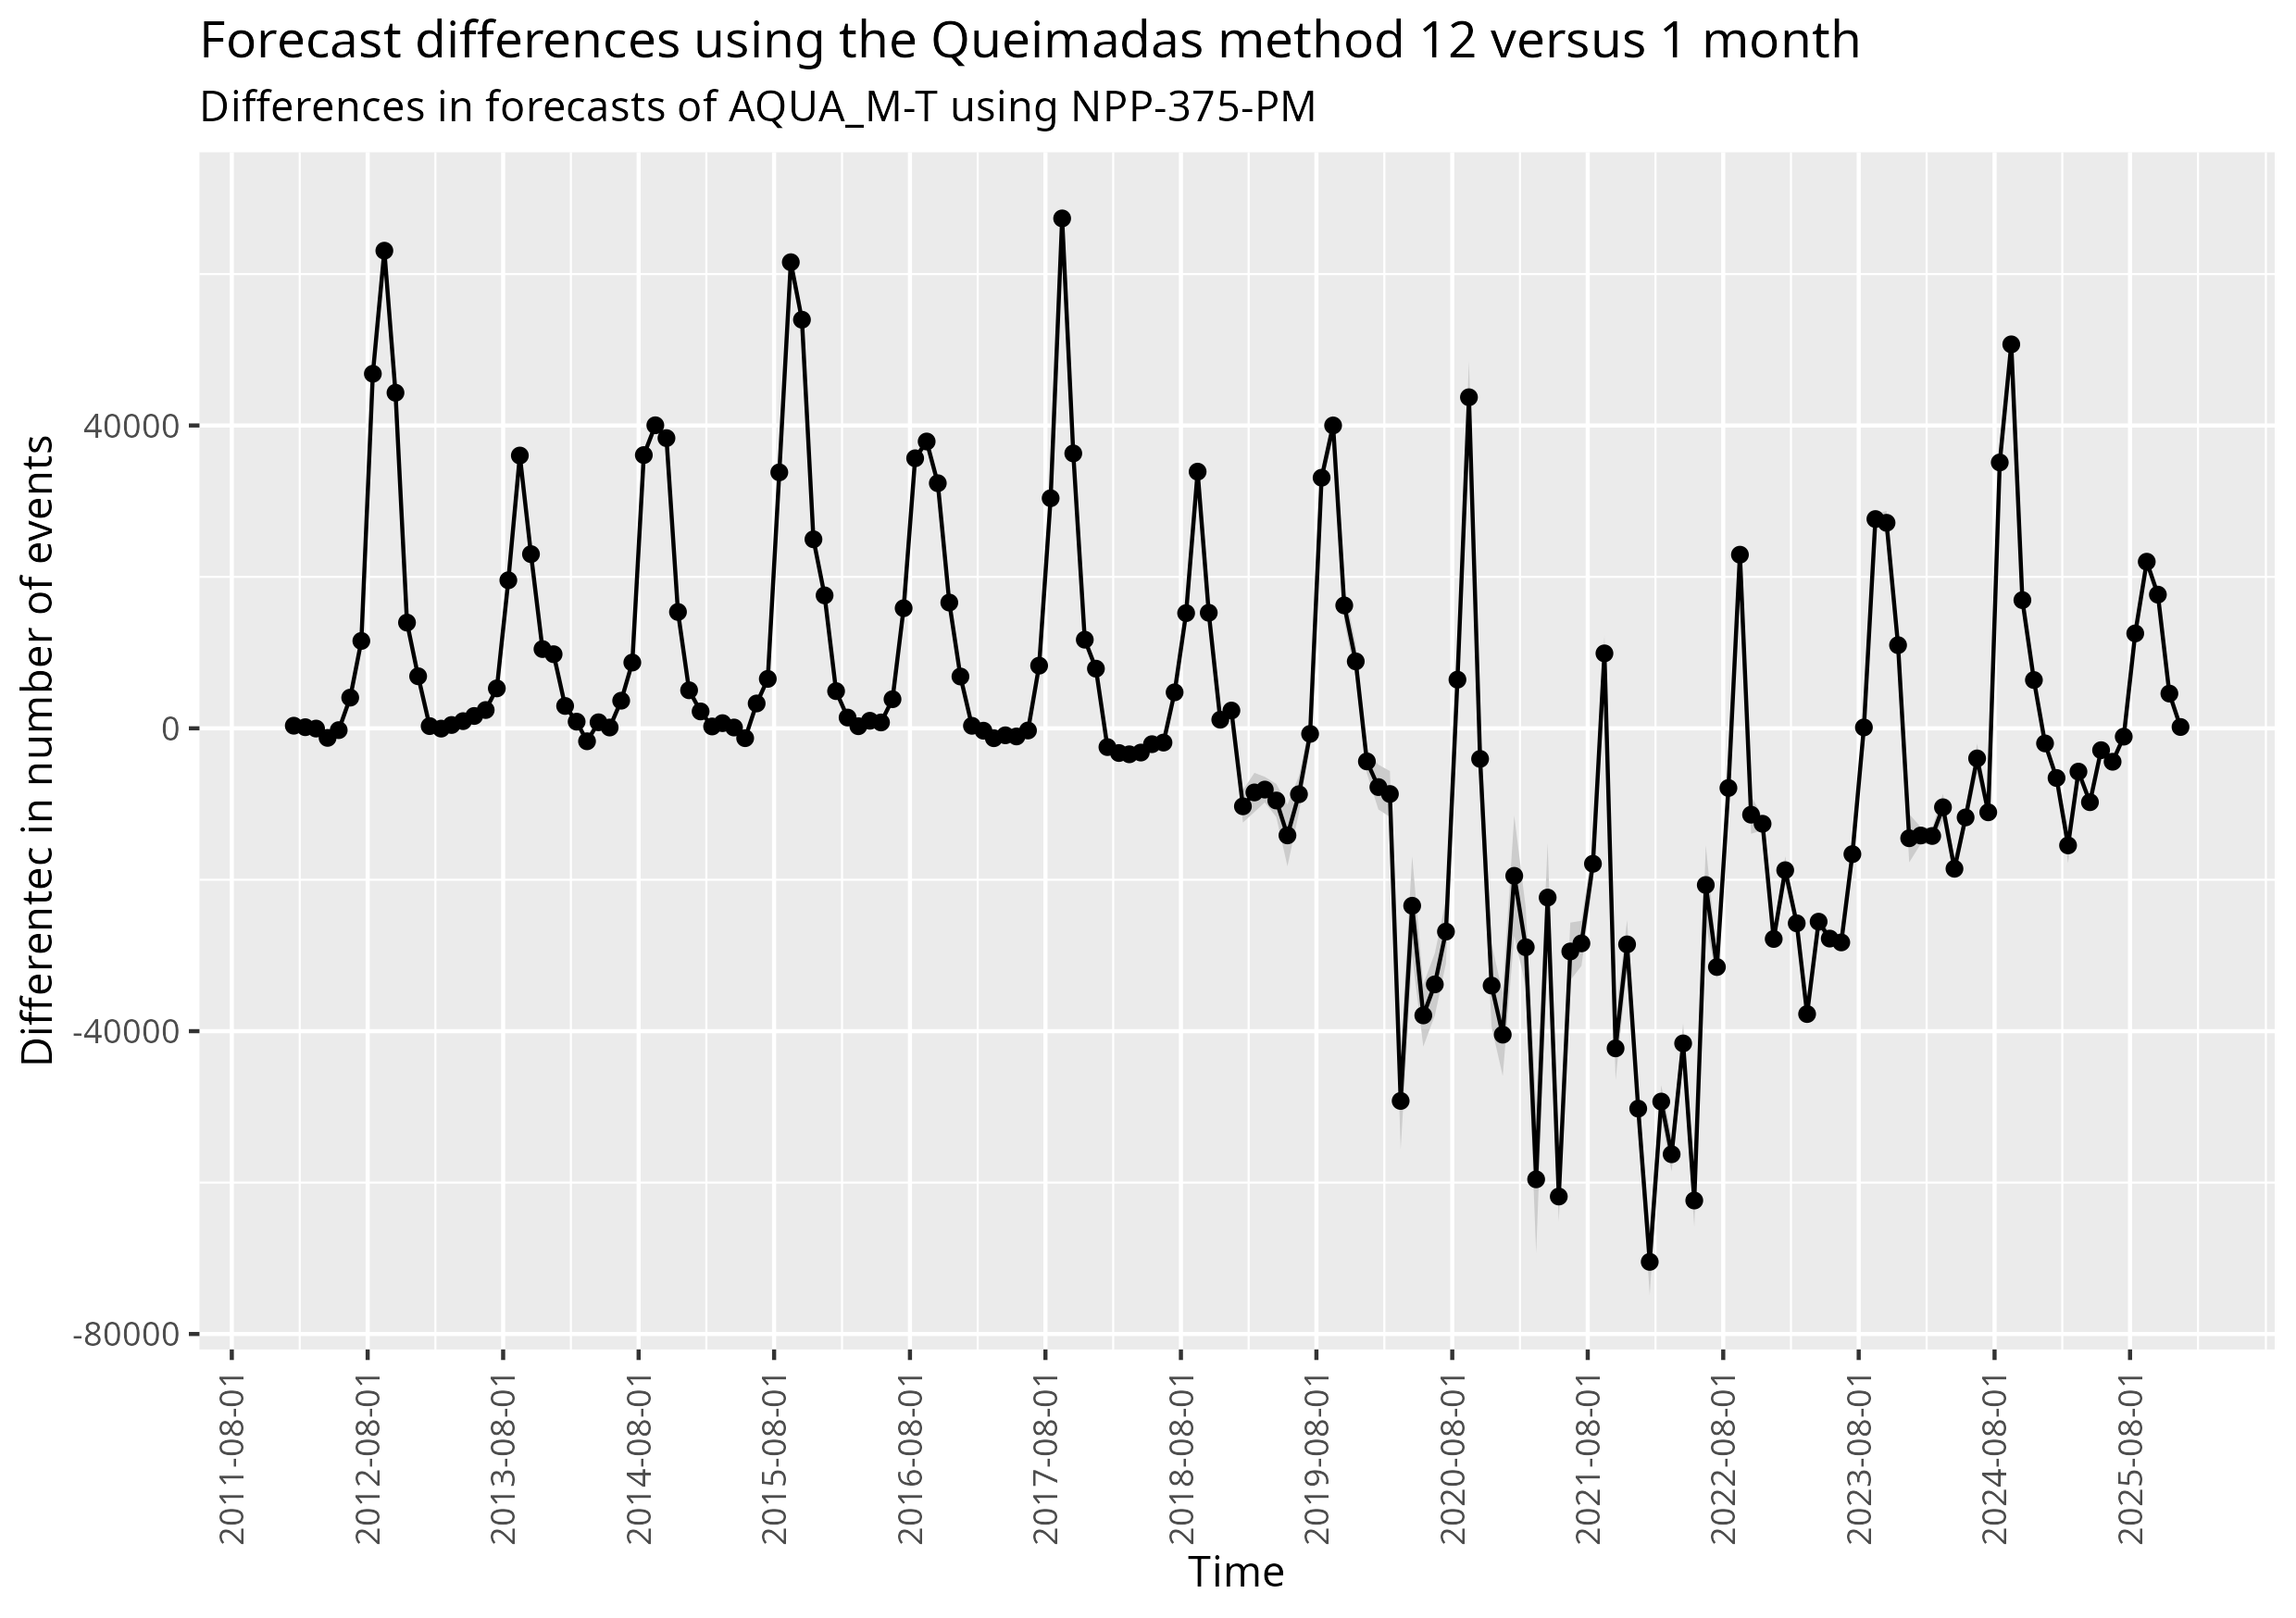
\includegraphics[scale=0.5]
    {figures/plot_forecast_differences_12_vs_1_AQUA_M-T_along_NPP-375-PM.png}
  \end{figure}
\end{frame}

\begin{frame}
  \frametitle{Forecast differences AQUA\_M-T vs. NOAA-12}
  \begin{figure}
    \centering
    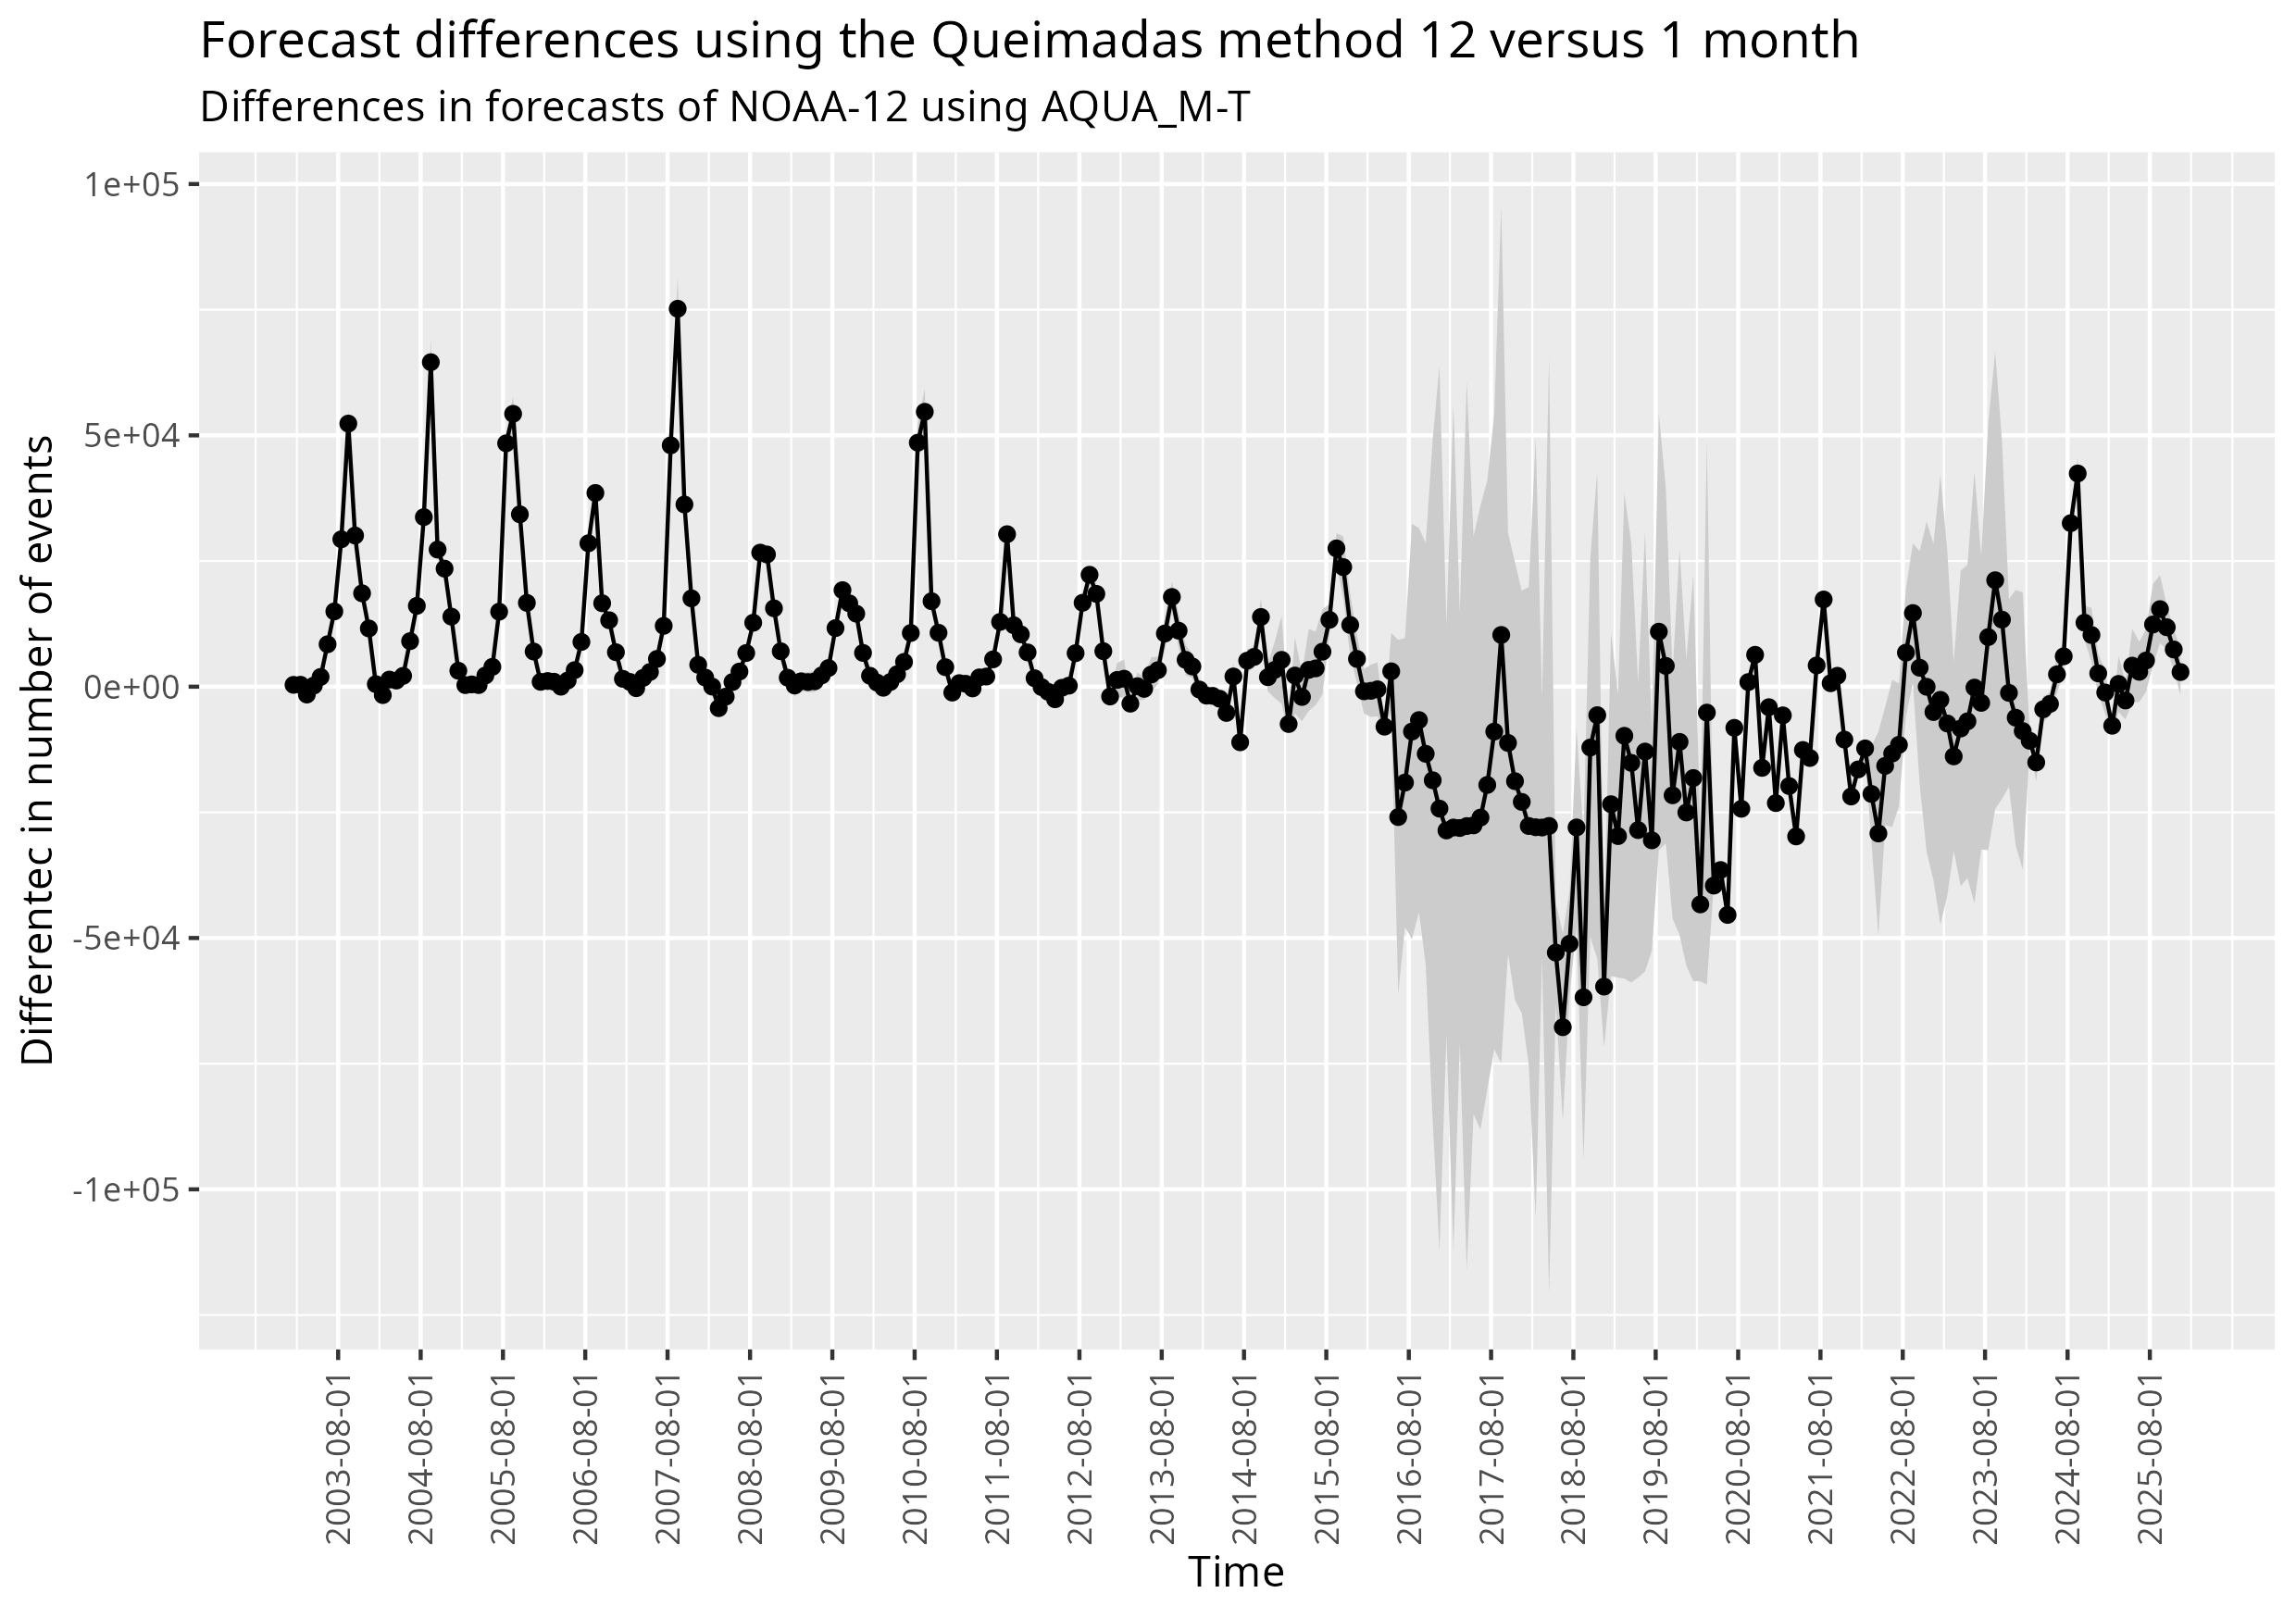
\includegraphics[scale=0.5]
    {figures/plot_forecast_differences_12_vs_1_NOAA-12_along_AQUA_M-T.png}
  \end{figure}
\end{frame}

\begin{frame}
  \frametitle{Forecast differences AQUA\_M-T vs. NPP-375PM}
  \begin{figure}
    \centering
    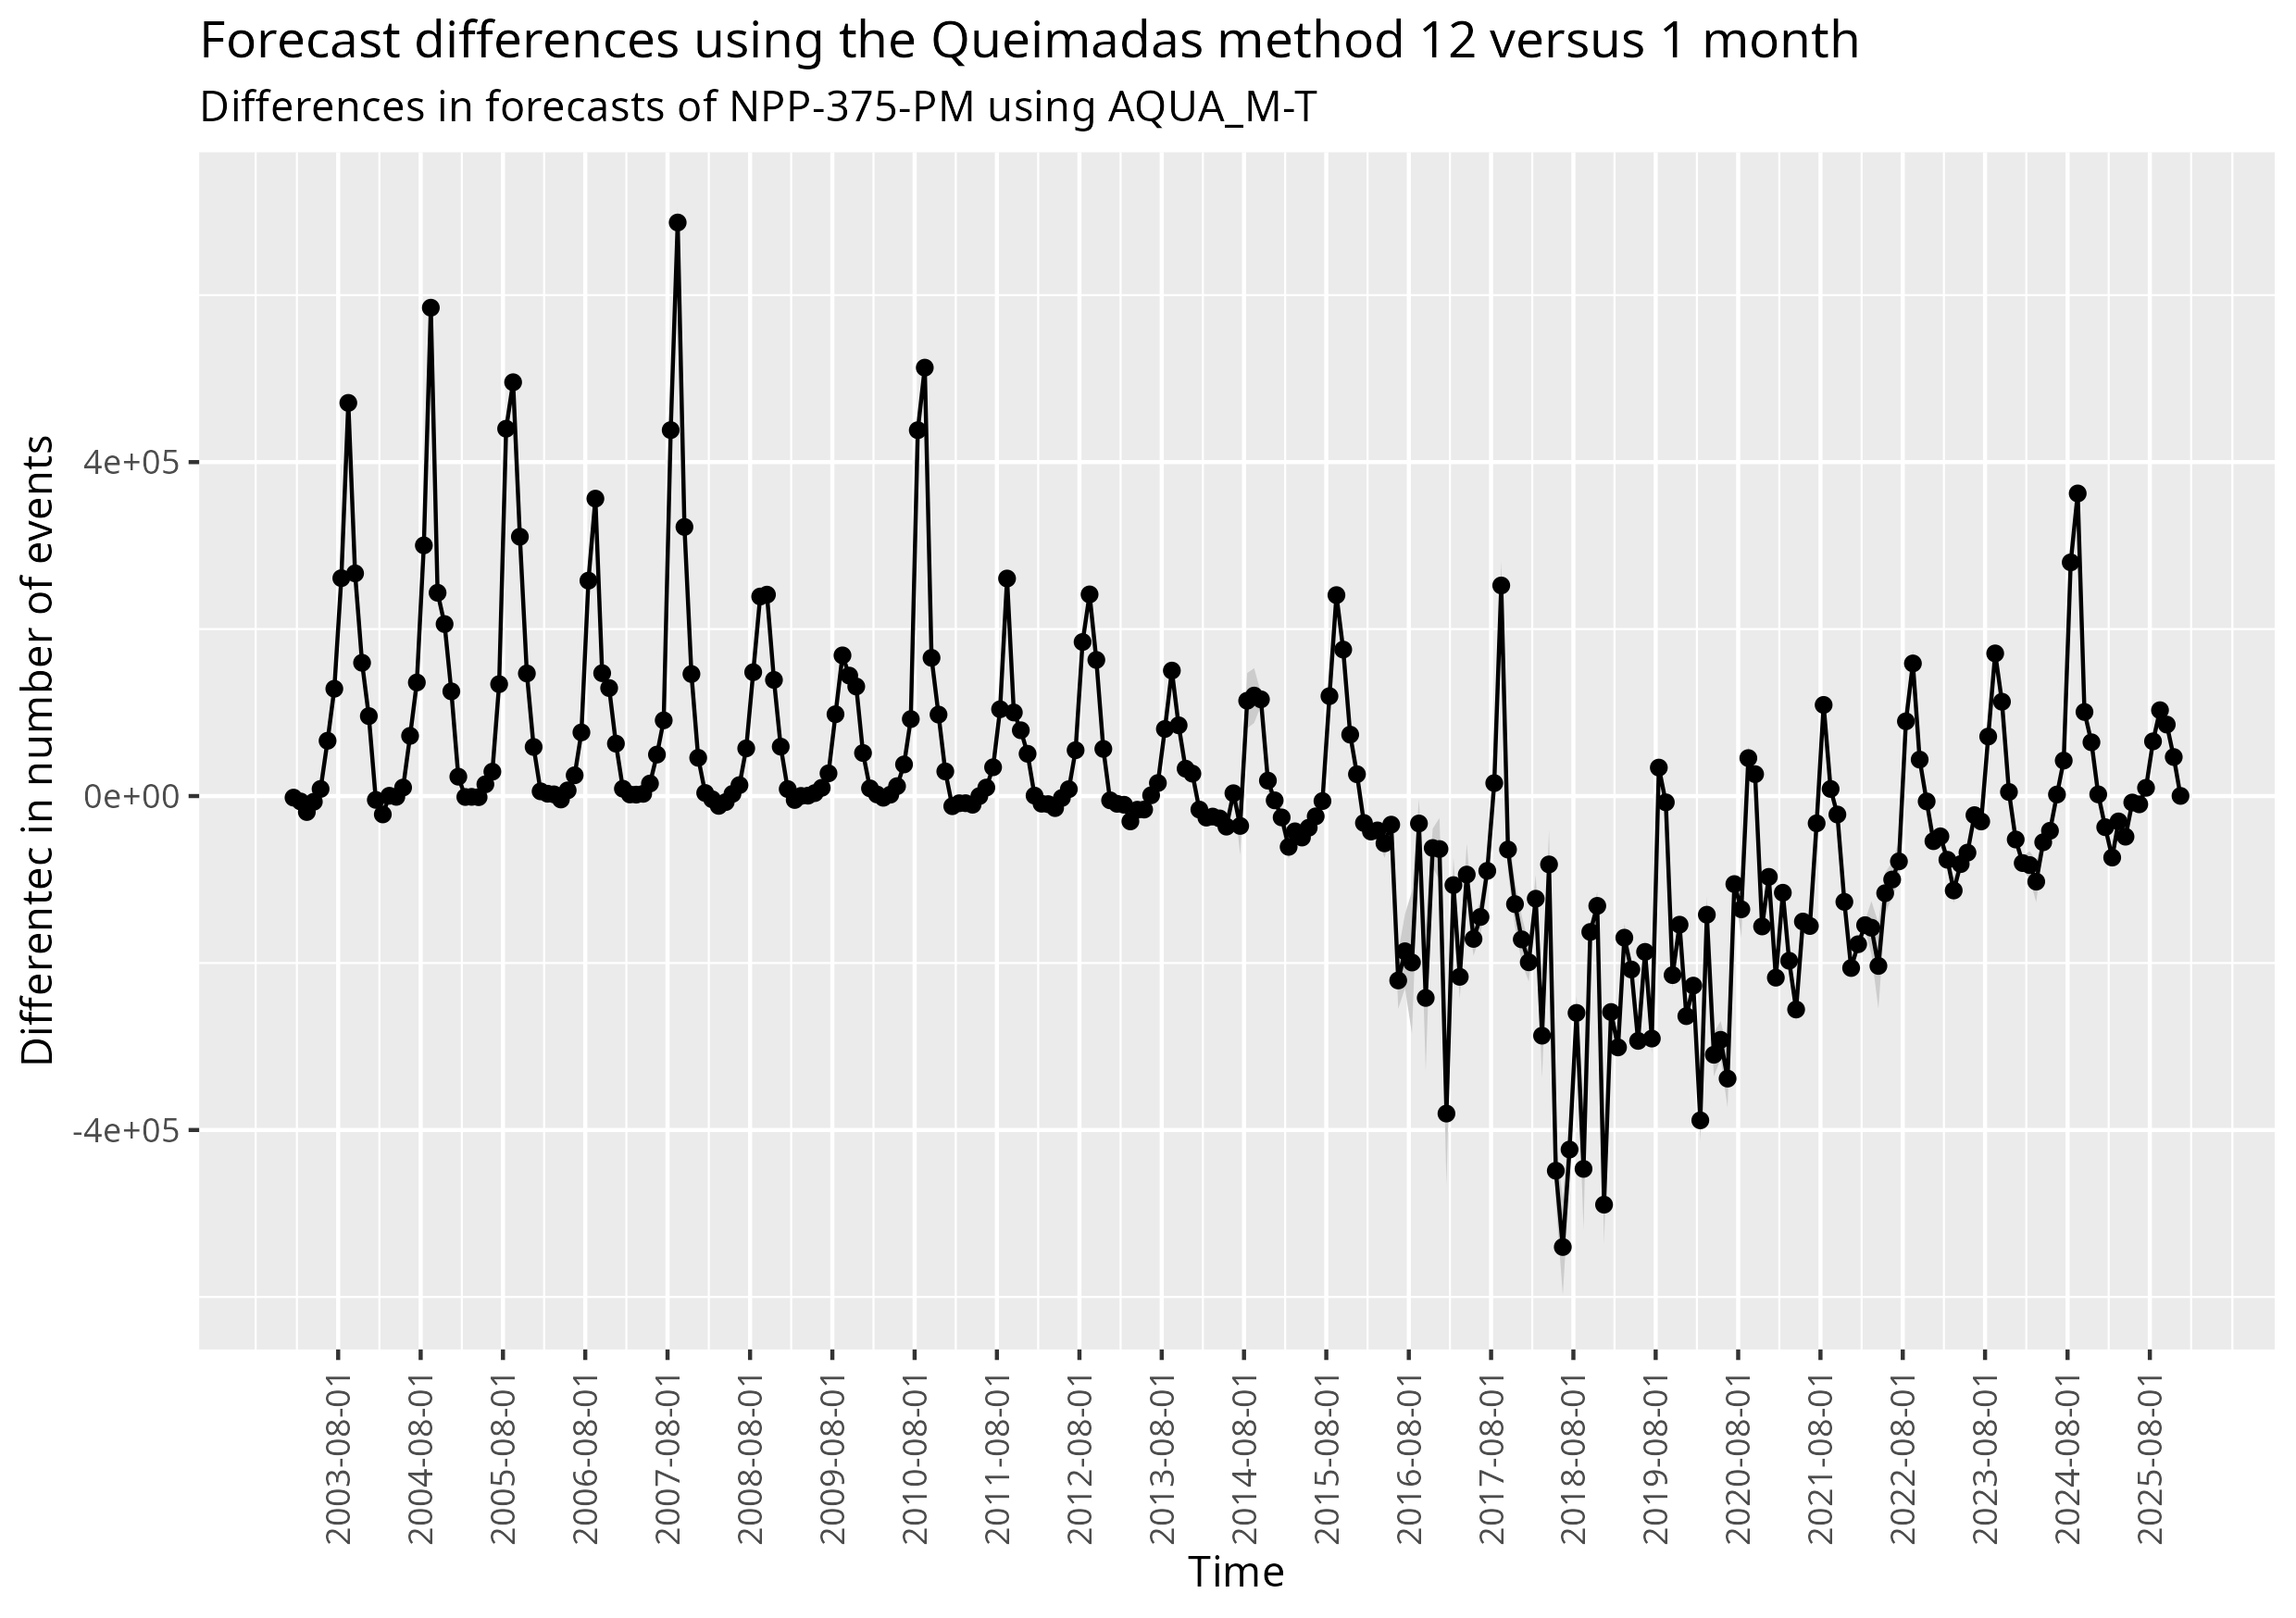
\includegraphics[scale=0.5]
    {figures/plot_forecast_differences_12_vs_1_NPP-375-PM_along_AQUA_M-T.png}
  \end{figure}
\end{frame}

\begin{frame}
  \frametitle{Forecast differences NPP-375D vs. NPP-375PM}
  \begin{figure}
    \centering
    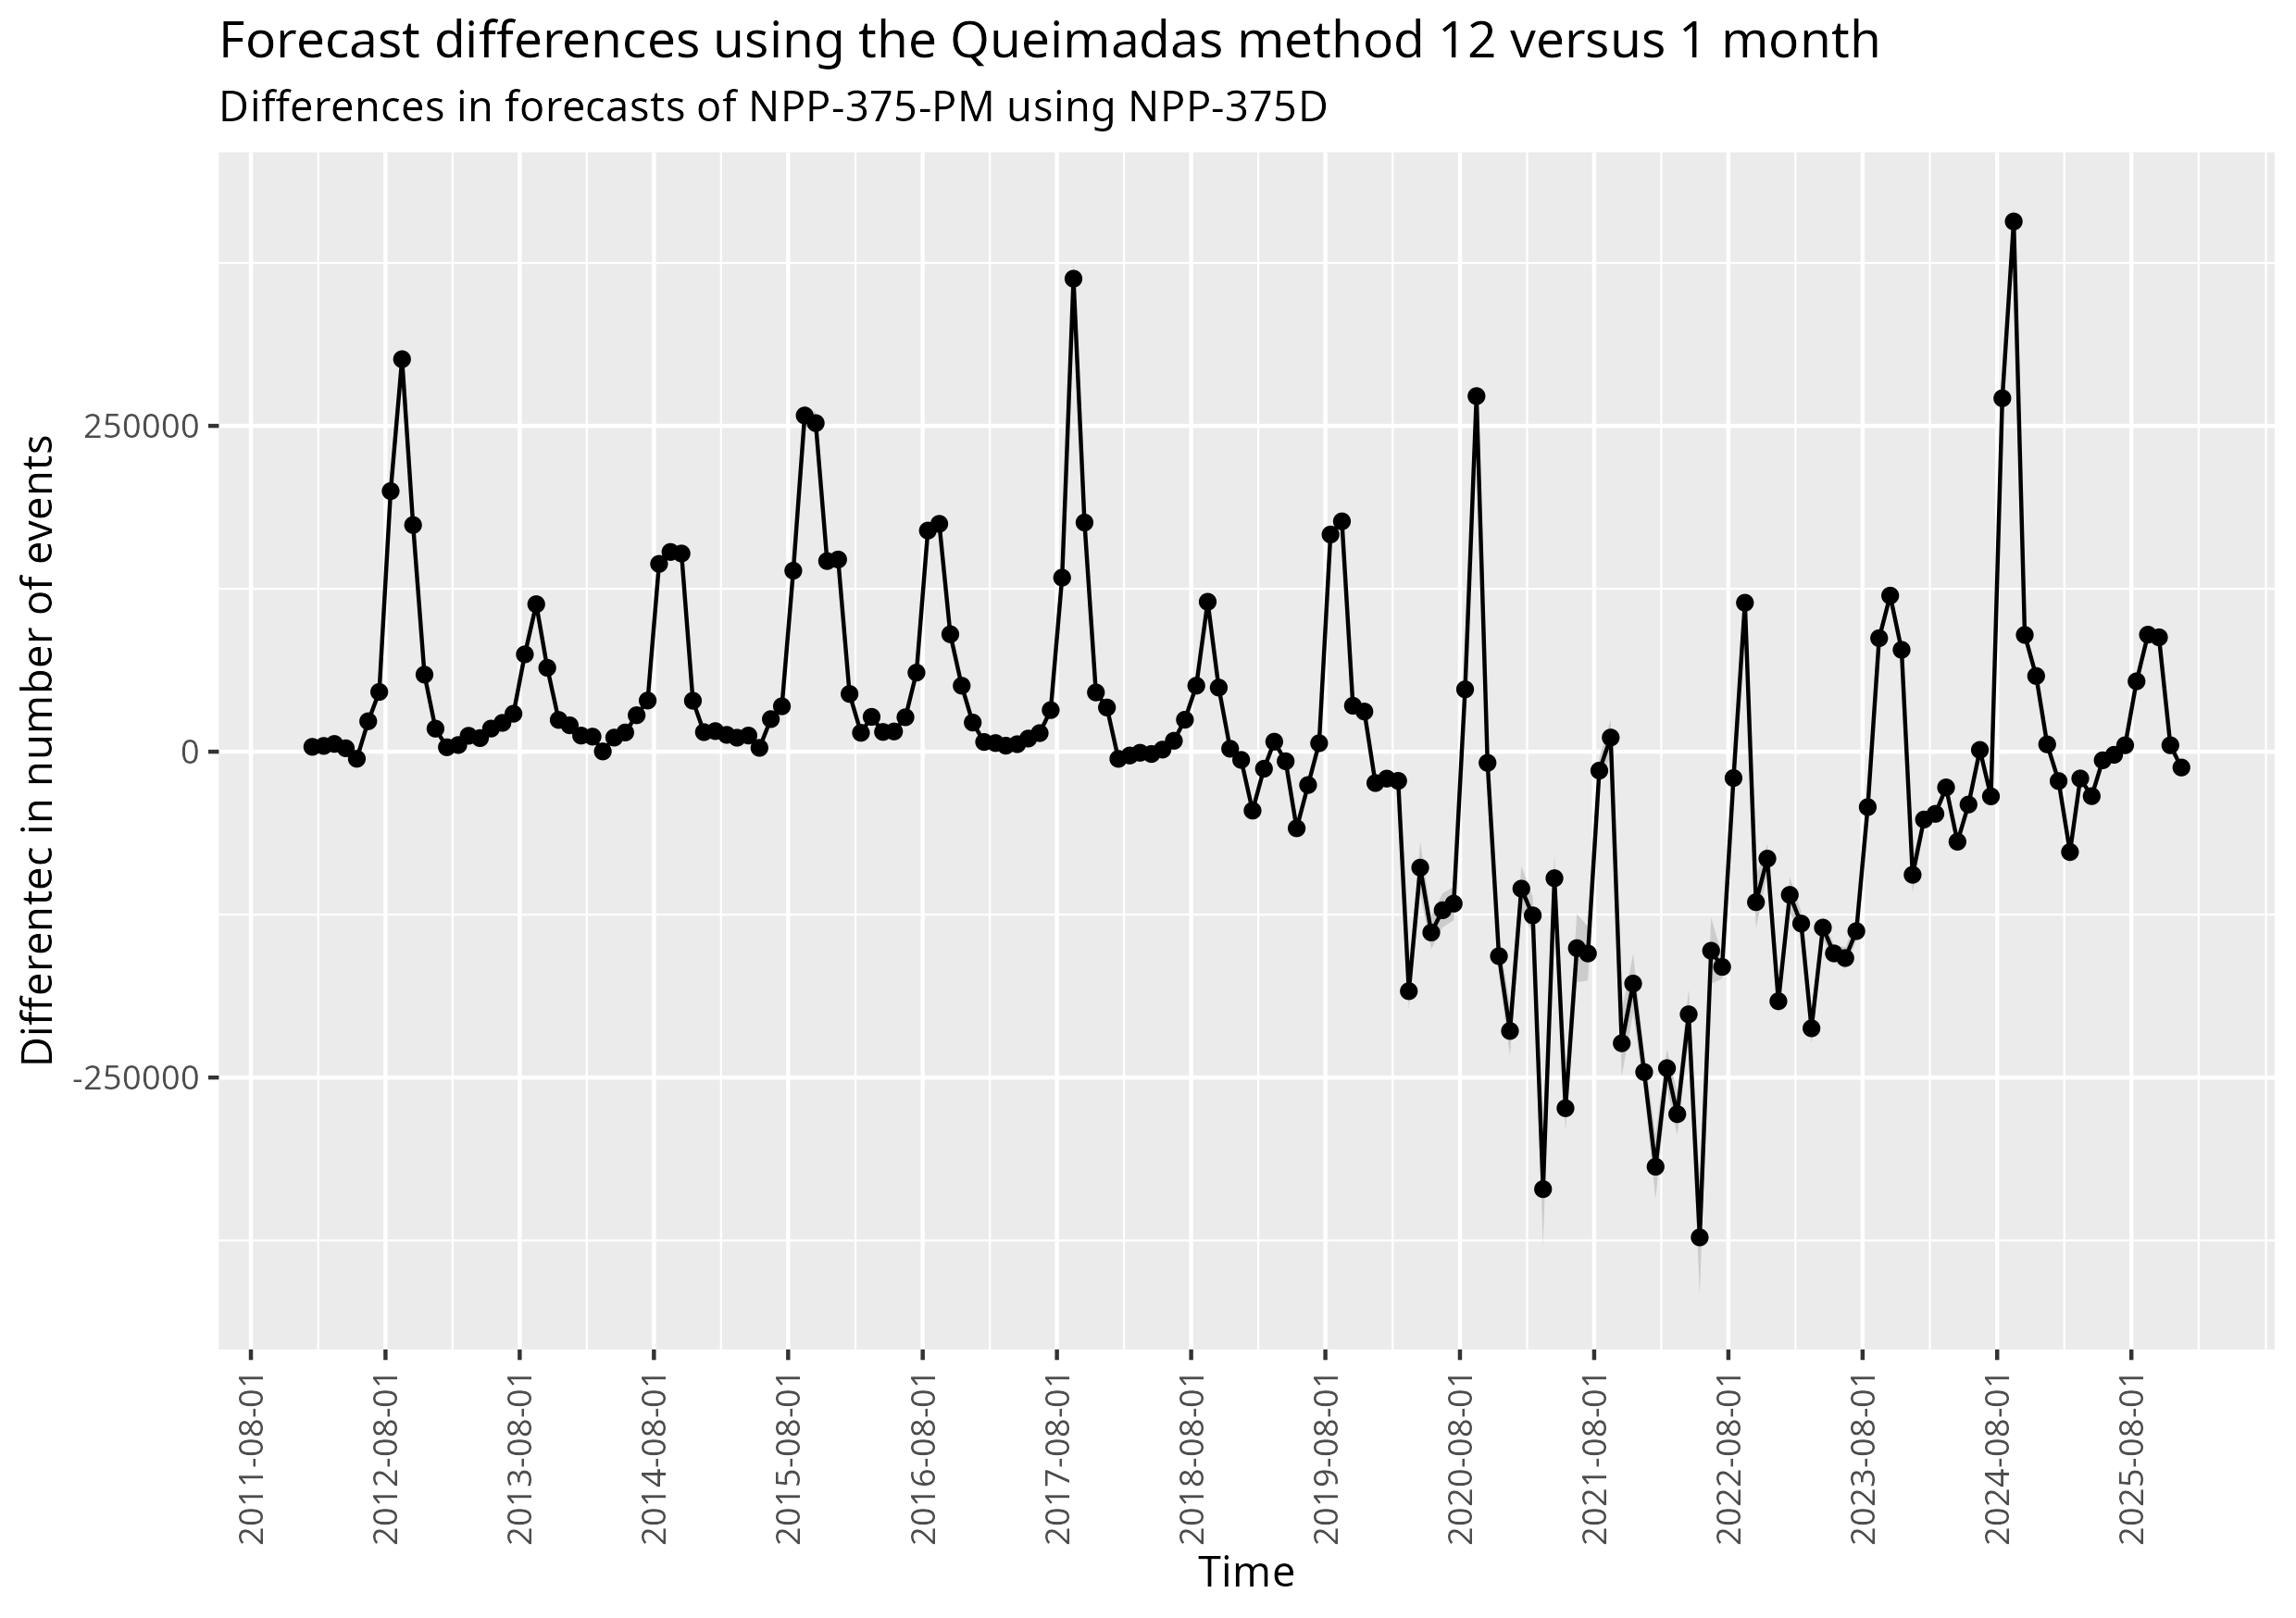
\includegraphics[scale=0.5]
    {figures/plot_forecast_differences_12_vs_1_NPP-375-PM_along_NPP-375D.png}
  \end{figure}
\end{frame}

\begin{frame}
  \frametitle{Forecast differences NPP-375PM vs. NPP-375D}
  \begin{figure}
    \centering
    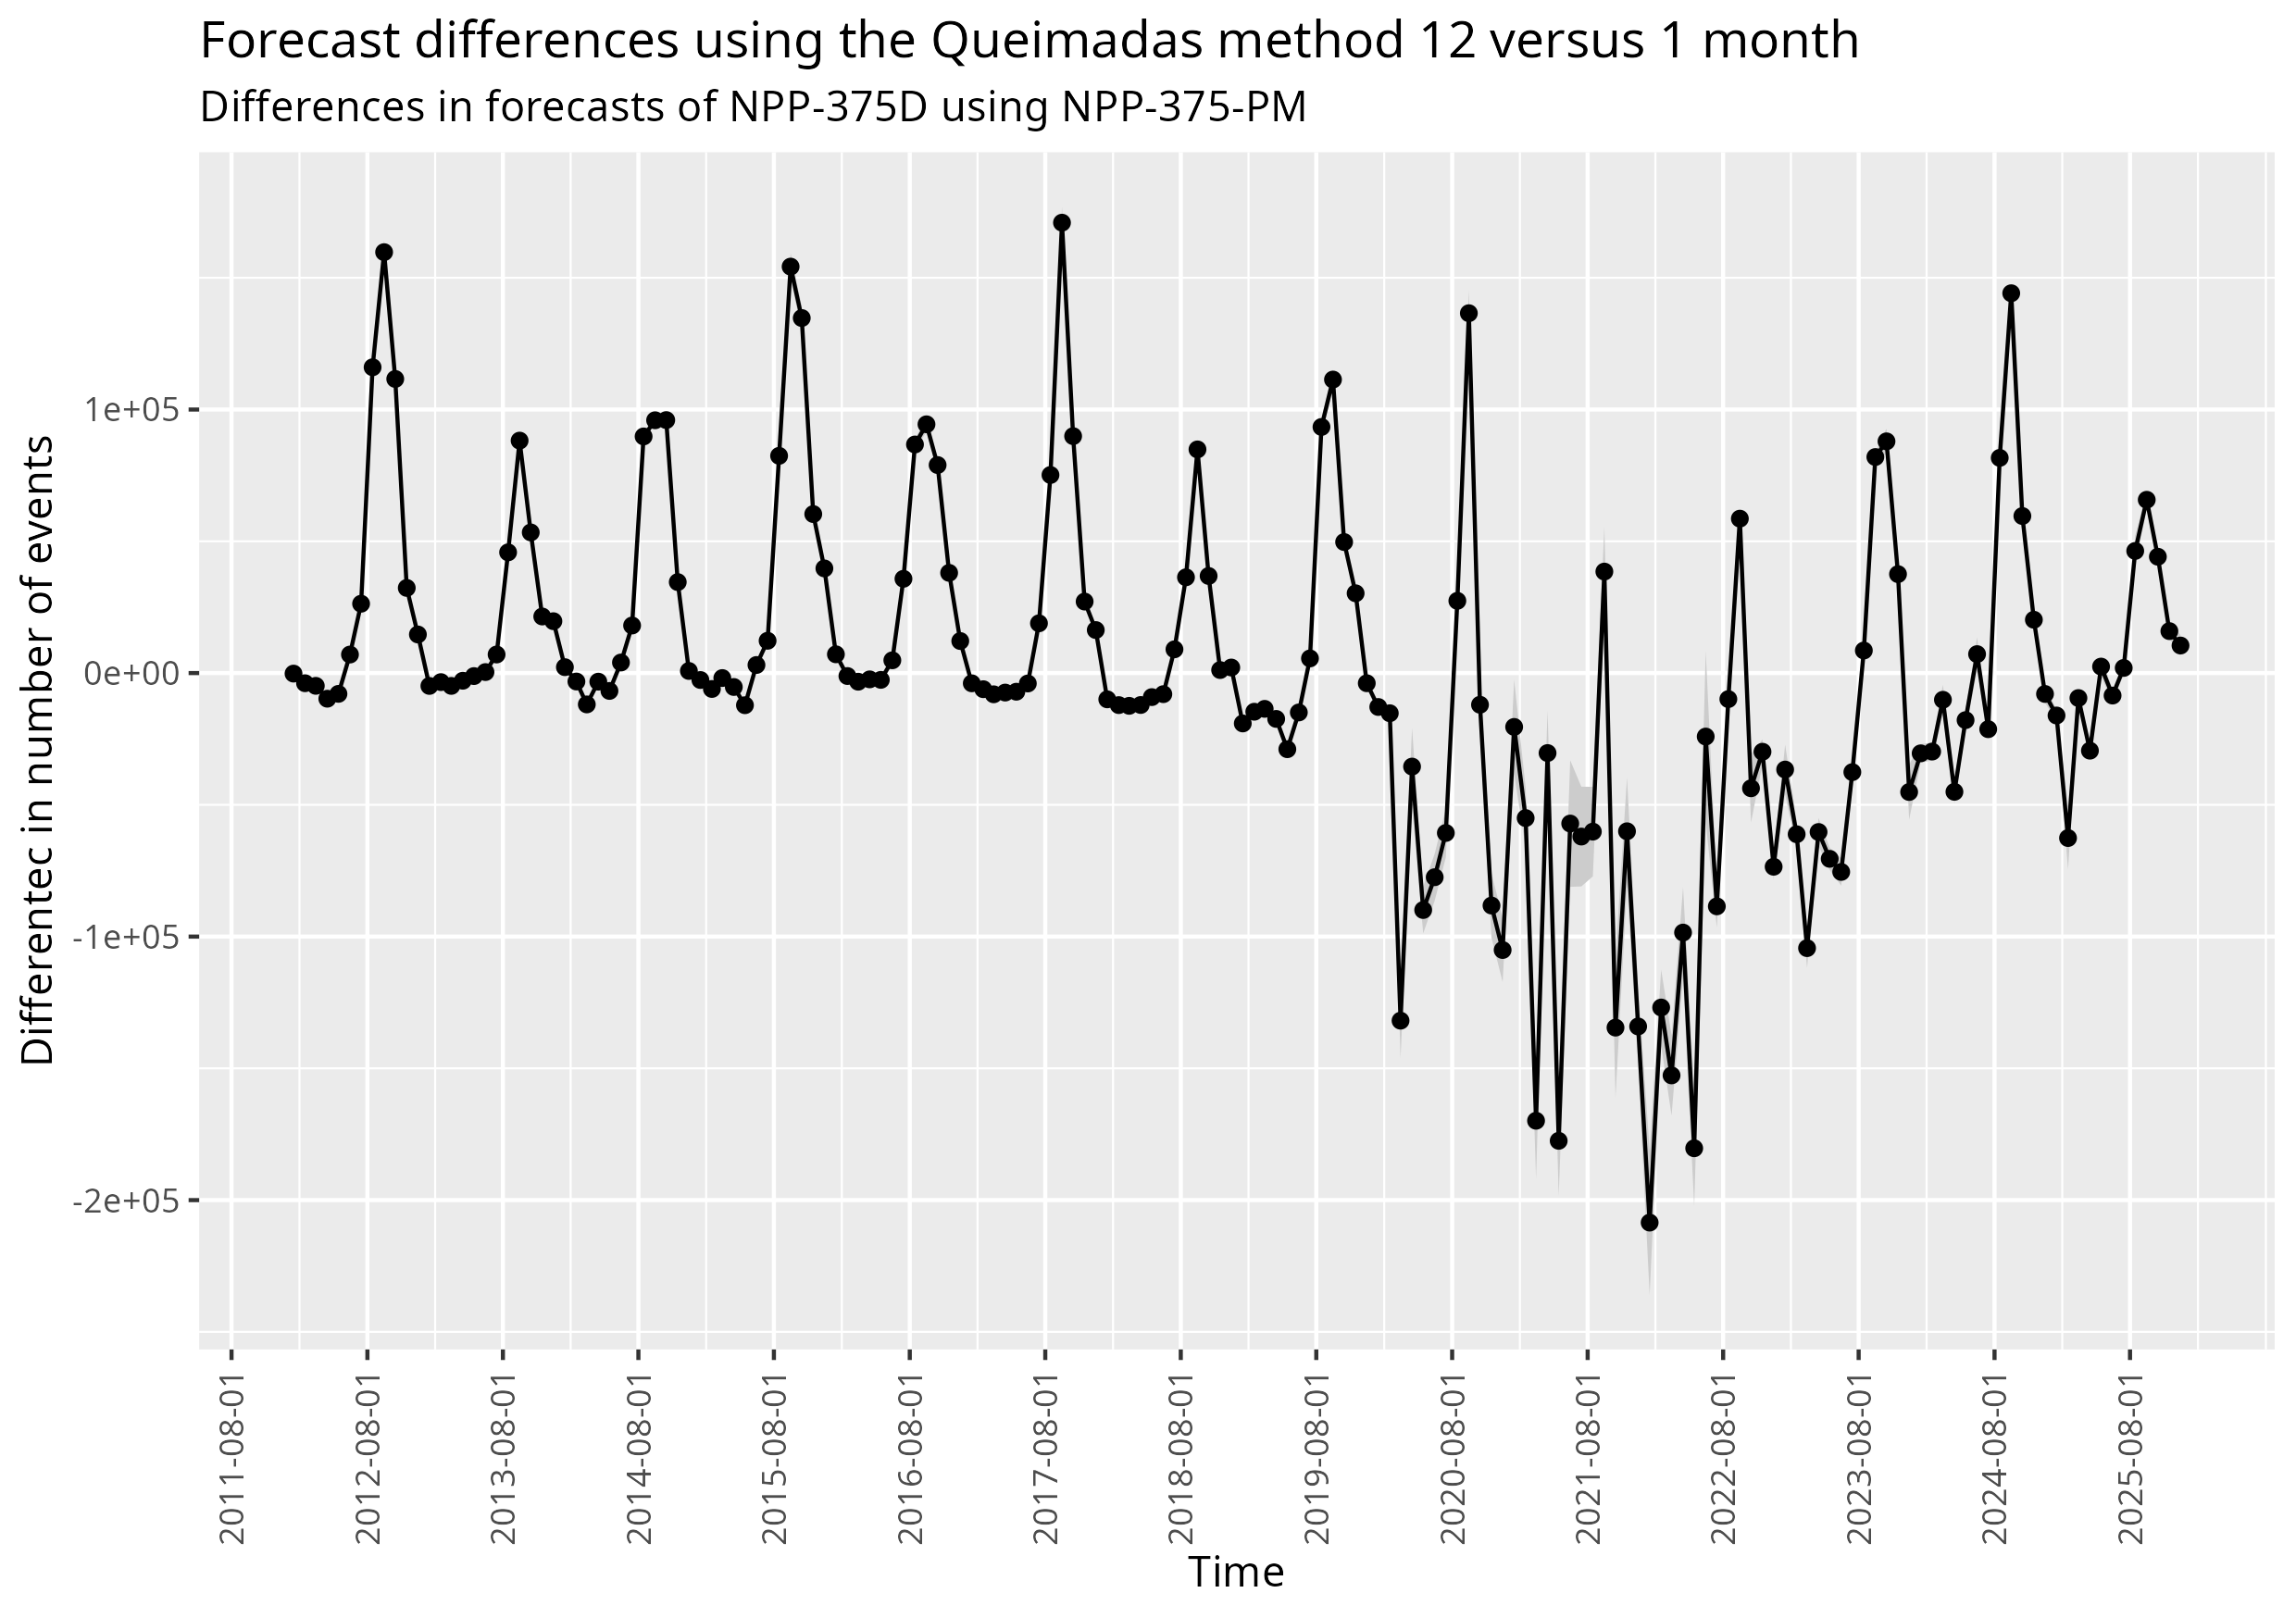
\includegraphics[scale=0.5]
    {figures/plot_forecast_differences_12_vs_1_NPP-375D_along_NPP-375-PM.png}
  \end{figure}
\end{frame}

\begin{frame}
  \frametitle{Forecast differences AQUA\_M-T vs. NPP-375D}
  \begin{figure}
    \centering
    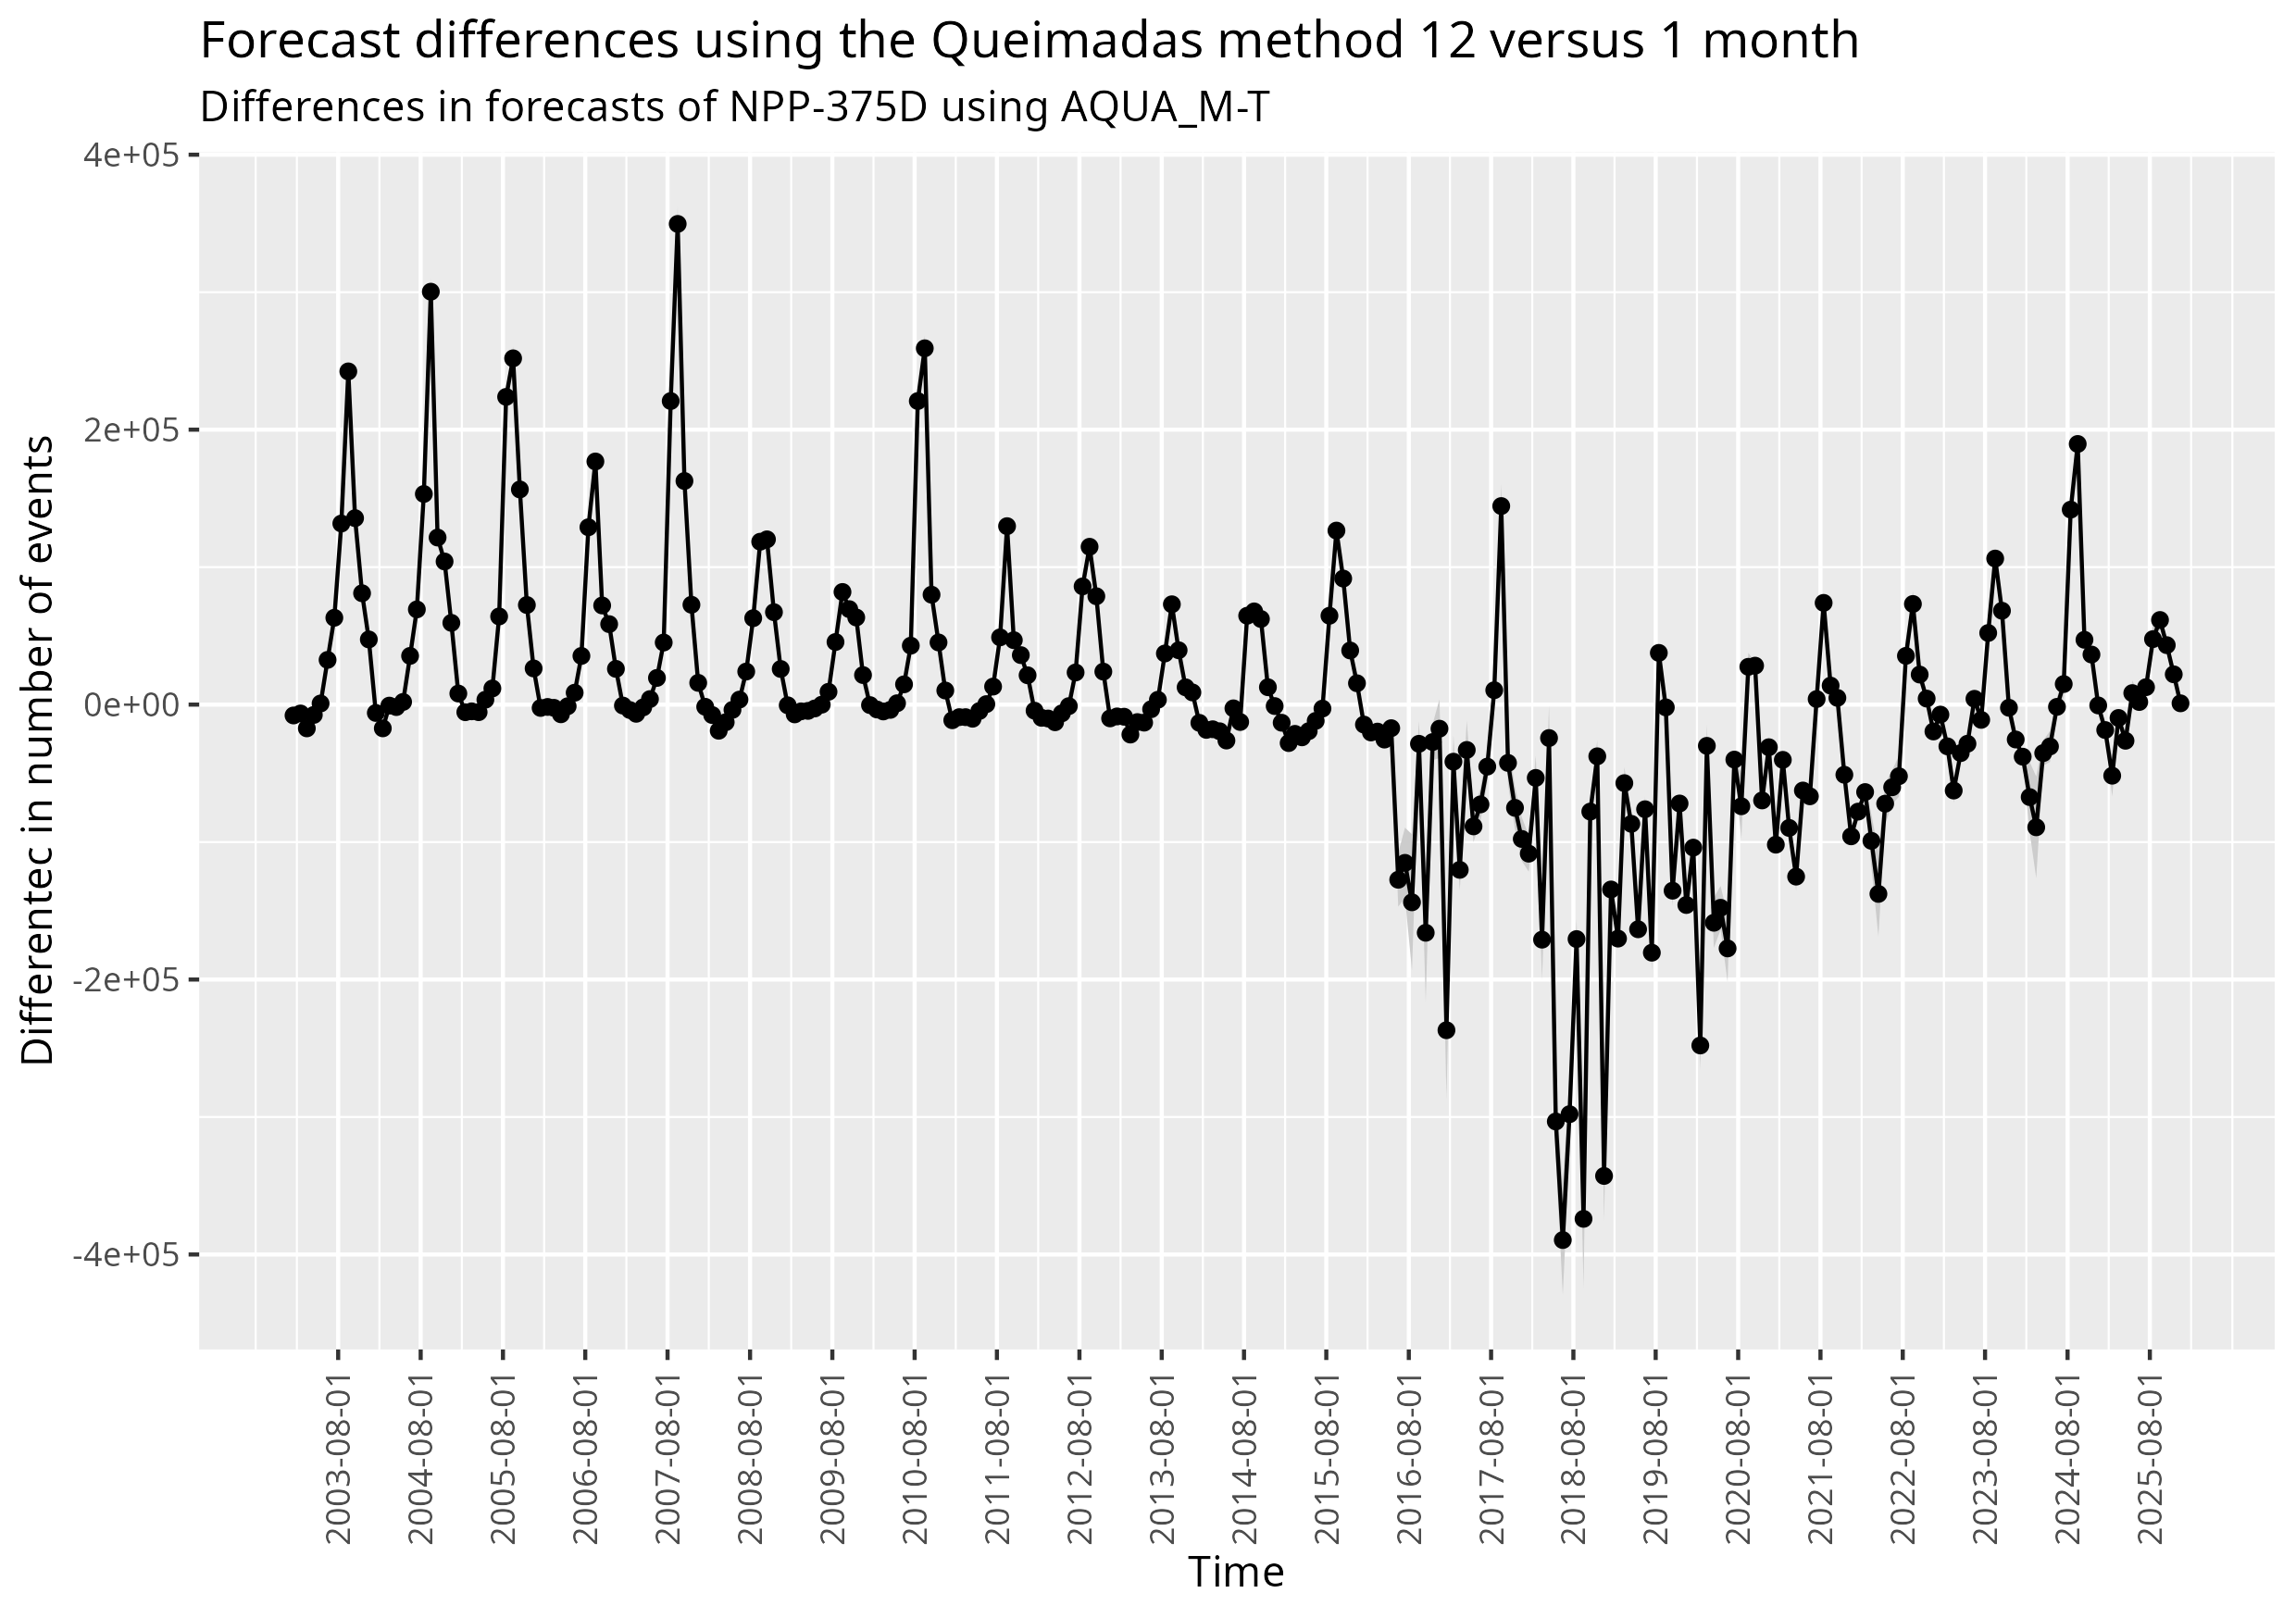
\includegraphics[scale=0.5]
    {figures/plot_forecast_differences_12_vs_1_NPP-375D_along_AQUA_M-T.png}
  \end{figure}
\end{frame}
